% This LaTeX document needs to be compiled with XeLaTeX.
\documentclass[10pt]{article}
\usepackage[utf8]{inputenc}
\usepackage{ucharclasses}
\usepackage{amsmath}
\usepackage{amsfonts}
\usepackage{amssymb}
\usepackage[version=4]{mhchem}
\usepackage{stmaryrd}
\usepackage{graphicx}
\usepackage[export]{adjustbox}
\graphicspath{ {./images/} }
\usepackage{caption}
\usepackage{multirow}
\usepackage[fallback]{xeCJK}
\usepackage{polyglossia}
\usepackage{fontspec}
\IfFontExistsTF{Noto Serif CJK KR}
{\setCJKmainfont{Noto Serif CJK KR}}
{\IfFontExistsTF{Apple SD Gothic Neo}
  {\setCJKmainfont{Apple SD Gothic Neo}}
  {\IfFontExistsTF{UnDotum}
    {\setCJKmainfont{UnDotum}}
    {\setCJKmainfont{Malgun Gothic}}
}}

\setmainlanguage{vietnamese}
\setotherlanguages{english}
\newfontfamily\vietnamesefont{CMU Serif}
\IfFontExistsTF{CMU Serif}
{\newfontfamily\lgcfont{CMU Serif}}
{\IfFontExistsTF{DejaVu Sans}
  {\newfontfamily\lgcfont{DejaVu Sans}}
  {\newfontfamily\lgcfont{Georgia}}
}
\setDefaultTransitions{\lgcfont}{}
\setTransitionsFor{Vietnamese}{\vietnamesefont}{\lgcfont}

\title{Chương 3. LIÊN KẾT HOÁ HỌC }

\author{}
\date{}


\def\AA{\mathring{\mathrm{A}}}

\begin{document}
\maketitle
\captionsetup{singlelinecheck=false}
\section*{HUÚNG DẤN GIẢI MỞ ĐẦU}
\section*{BÀI 1. NHẬP MÔN HOÁ HỌC}
1.1. - Đơn chất: $\mathrm{Cu}, \mathrm{O}_{2}, \mathrm{~N}_{2}, \mathrm{O}_{3}, \mathrm{Al}, \mathrm{He}, \mathrm{H}_{2}$.

\begin{itemize}
  \item Hợp chất: $\mathrm{HCl}, \mathrm{H}_{2} \mathrm{SO}_{4}, \mathrm{NH}_{4} \mathrm{NO}_{3}, \mathrm{HCl}$.\\
1.2. - Hiện tượng vật lí: $\mathrm{a}, \mathrm{c}, \mathrm{d}$.
  \item Hiện tượng hoá học: b.\\
1.3. - Hiện tượng hoá học: $\mathrm{a}, \mathrm{b}, \mathrm{d}, \mathrm{f}$.
  \item Hiện tượng vật lí: $\mathrm{c}, \mathrm{e}, \mathrm{g}$.\\
1.4. - Hiện tượng hoá học: $\mathrm{b}, \mathrm{d}$.
  \item Hiện tượng vật lí: $a, c, e$.\\
1.5. - Hiện tượng hoá học: b, c, e.
  \item Hiện tượng vật lí: $\mathrm{a}, \mathrm{d}$.\\
1.6. - Quá trình biến đổi vật lí: "người ta đập đá vôi thành những cục nhỏ có kích thước thích hợp", "thêm nước vào nước vôi đặc ta được nước vôi loãng".
  \item Quá trình biến đổi hoá học: "nung đá vôi ta được vôi sống và khí carbon dioxide", "khuấy vôi sống với ît nước ta được nước vôi đặc".\\
1.7. - Quá trình biến đổi vậtlí: "thanh sắt nung nóng, dát mỏng, kéo dài thành dây sắt".
  \item Quá trình biến đổi hoá học: "tiếp tục nung nóng thành chất bột màu nâu".\\
1.8.\\
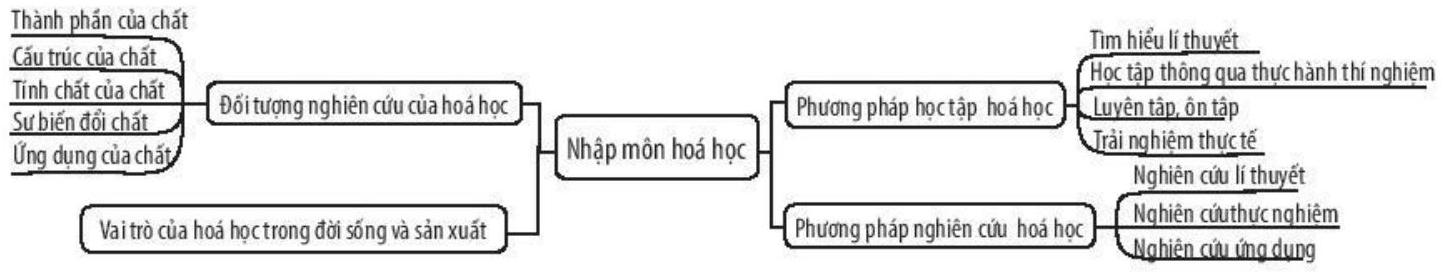
\includegraphics[max width=\textwidth, center]{2025_10_23_57761e23b8c46a11c3efg-01}\\
1.9.
\end{itemize}

\begin{center}
\begin{tabular}{|l|l|}
\hline
Phương pháp nghiên cứu lí thuyết & Tìm hiểu về cây chanh, công dụng và tác dụng dược lí của chanh cũng như hoạt tính kháng oxi hoá, kháng vi sinh vật của nó thông qua các công bố khoa học trong và ngoài nước. \\
\hline
Phương pháp nghiên cứu thực nghiệm & \begin{tabular}{l}
Thu hái mẫu vỏ chanh tại vườn chanh. \\
Khảo sát sự trích li tinh dầu bằng phương pháp chưng cất lôi cuốn hơi nước. \\
\end{tabular} \\
\hline
Phương pháp nghiên cứu ứng dụng & Thử hoạt tính kháng oxi hoá, thử hoạt tính kháng vi sinh vật. \\
\hline
\end{tabular}
\end{center}

1.10.

\begin{center}
\begin{tabular}{|l|l|}
\hline
Xác định vấn đề nghiên cứu & Nghiên cứu thành phần hoá học, hoạt tính kháng oxi hoá và hoạt tính kháng khuẩn của tinh dầu vỏ chanh. \\
\hline
Nêu giả thuyết khoa học & Tinh dầu vỏ chanh có hoạt tính kháng oxi hoá và hoạt tính kháng khuẩn. \\
\hline
Thực hiện nghiên cứu (li thuyết, thực nghiệm, ứng dụng) & \begin{tabular}{l}
Tìm hiểu về cây chanh, công dụng và tác dụng dược lí của chanh cũng như hoat tính kháng oxi hoá, kháng vi sinh vật của nó thông qua các công bố khoa học trong và ngoài nước. \\
Thu hái mẫu vỏ chanh tại vườn chanh. \\
Khảo sát sự trích li tinh dầu bằng phương pháp chưng cất lôi cuốn hơi nước. \\
Thử hoạt tính kháng oxi hoá, thử hoạt tính kháng vi sinh vật. \\
\end{tabular} \\
\hline
Viết báo cáo: thảo luận kết quả và kết luận vấn đề & \begin{tabular}{l}
So sánh các chỉ số vật lí, thành phần hoá học, hoạt tính kháng oxi hoá, kháng vi sinh vật của tinh dầu vỏ chanh Úc, Mỹ và vỏ chanh giấy. \\
Công bố: tinh dầu vỏ chanh giấy có đường kính vòng vô khuẩn cao nhất, sau đó là tinh dầu vỏ chanh Mỹ và thấp nhất là của tinh dầu vỏ chanh Úc. Nổi bật nhất là tinh dầu vỏ chanh giấy cho đường kính vòng vô khuẩn cao nhất với vi khuẩn thử nghiệm Shigella flexneri NCDC 2747-7. \\
\end{tabular} \\
\hline
\end{tabular}
\end{center}

\section*{Chưong 1. CẤU TẠO NGUYÊN TỬ}
\section*{Bài 2. THÀNH PHẦN CỦA NGUYÊN TỬ'}
2.1. Đáp án $D$.\\
2.2. Đáp án A .\\
2.3. Đáp án $C$.\\
2.4. Đáp án $B$.\\
2.5. Đáp án $C$ vì số proton trong $R=$ số electron trong $R=\frac{-41,6 \times 10^{-19}}{-1,602 \times 10^{-19}} \approx 26$.\\
2.6. Đáp án A.\\
2.7. Đáp án A .\\
2.8. Đáp án $B$.\\
2.9. Đáp án A .\\
2.10. Đáp án B.\\
(1) sai vì hydrogen không có neutron.\\
(2) sai vì khối lượng nguyên tử tập trung ở phần hạt nhân nguyên tử.\\
(3) đúng.\\
(4) sai vì hạt nhân nguyên tử không chứa electron.\\
(5) đúng.\\
2.11. Đa số hạt $\alpha$ bay xuyên qua lá vàng mỏng với hướng di chuyển không đổi. Một số hạt $\alpha$ bị lệch hướng, chứng tỏ có va chạm trước khi bay ra khỏi lá vàng, một số hạt $\alpha$ bị lệch hướng do chịu tác động của một lượng lớn điện tích dương tập trung trong một không gian rất nhỏ ở trung tâm nguyên tử vàng. Các electron của nguyên tử quay quanh lõi trung tâm, giống như các hành tinh quay quanh Mặt Trời. Phần lõi này được gọi là hạt nhân nguyên tử.\\
2.12. 1. cathode; 2. nguyên tử; 3. proton; 4. neutron; 5. electron; 6. neutron.\\
2.13. Tia âm cực là dòng electron mang điện tích âm.\\
2.14. Các electron không khác nhau về bản chất trong các môi trường khác nhau.\\
2.15. Nguyên tử trung hoà về điện vì trong nguyên tử, số proton bằng số electron, hay nói cách khác số đơn vị điện tích dương bằng số đơn vị điện tích âm.\\
2.16. Gọi $\mathrm{p}, \mathrm{n}$ và e lần lượt là số proton, neutron và electron của X .

Theo đề bài, ta có hệ phương trình: $\left\{\begin{array}{l}2 p+n=52 \\ 2 p-n=16\end{array}\right.$\\
Giải hệ phương trình ta được: $\mathrm{p}=17, \mathrm{n}=18$.\\
Vậy trong $X$ có 17 electron và 18 neutron.\\
2.17. Gọi $p, n$ và e lần lượt là số proton, neutron và electron của Y.

Theo đề bài, ta có hệ phương trình: $\left\{\begin{array}{l}2 p+n=36 \\ n=\frac{1}{2}(36-p)\end{array}\right.$\\
Giải hệ phương trình ta được: $\mathrm{p}=12, \mathrm{n}=12$.\\
Vậy trong Y có: 12 proton, 12 electron và 12 neutron.\\
2.18. \% hạt không mang điện $=33,33 \% \Rightarrow$ số neutron $=n=33,33 \% \times 21=7$ (1)\\
$2 p+n=21(2)$\\
Thế (1) vào (2) $\Rightarrow \mathrm{p}=\mathrm{e}=\frac{21-7}{2}=7$.\\
Vậy nguyên tử $N$ có số đơn vị điện tích hạt nhân là 7 .\\
2.19. Tổng số hạt mang điện trong hợp chất MgO là $40 \rightarrow 2 \mathrm{p}_{\mathrm{Mg}}+2 \mathrm{p}_{\mathrm{o}}=40$ (1)

Số hạt mang điện trong nguyên tử Mg nhiều hơn số hạt mang điện trong nguyên tử O là 8 .\\
$\Rightarrow 2 \mathrm{p}_{\mathrm{Mg}}-2 \mathrm{p}_{\mathrm{o}}=8(2)$\\
Giải hệ (1), (2) $\Rightarrow \mathrm{p}_{\mathrm{Mg}}=12, \mathrm{p}_{\mathrm{o}}=8 \Rightarrow$ Điện tích hạt nhân của Mg là +12 ; Olà +8 .\\
2.20. Thành phần \% khối lượng electron trong nguyên tử helium:

$$
\frac{2 \times 9,11 \times 10^{-28}}{2 \times 1,673 \times 10^{-24}+2 \times 1,675 \times 10^{-24}+2 \times 9,11 \times 10^{-28}} \times 100 \%=0,0272 \%
$$

2.21*.\\
a) Hạt nhân như vậy có tiết diện hình tròn bằng $\frac{1}{10^{8}}$ tiết diện của nguyên tử. Vì đường kính tỉ lệ với căn bậc hai của diện tích hình tròn nên hạt nhân có đường kính vào khoảng $\frac{1}{10^{4}}$ đường kính của nguyên tử.\\
b) Với giả thiết như đề bài thì đường kính nguyên tử sẽ là:

$$
3 \times 10^{4} \mathrm{~cm}=30000 \mathrm{~cm}=300 \mathrm{~m}
$$

2.22*.

Thể tích 1 mol nguyên tử calcium $=\frac{M}{d} \times 74 \%=\frac{40}{1,55} \times 74 \%\left(\mathrm{~cm}^{3}\right)$\\
Thể tích 1 nguyên tử calcium $=\frac{\frac{40}{1,55} \times 74 \%}{6,023 \times 10^{23}}\left(\mathrm{~cm}^{3}\right)$\\
Bán kính nguyên tử calcium $=\sqrt[3]{\frac{3 \times \frac{\frac{40}{1,55} \times 74 \%}{6,023 \times 10^{23}}}{4 \pi}}=1,96 \times 10^{-8} \mathrm{~cm}$\\
2.23*.

Khối lượng của 1 nguyên tử Fe: $\frac{56}{6,023 \times 10^{23}}($ gam $)$.\\
Thể tích của 1 nguyên tử $\mathrm{Fe}: \mathrm{V}=\frac{4}{3} \pi \mathrm{r}^{3} \approx \frac{4}{3} \pi\left(1,28 \times 10^{-8}\right)^{3}\left(\mathrm{~cm}^{3}\right)$.\\
Khối lượng riêng của Fe: $d=\frac{m}{V} \approx 10,59\left(\mathrm{~g} / \mathrm{cm}^{3}\right)$.\\
Fe chiếm $74 \%$ thể tích trong tinh thể nên khối lượng riêng thực tế của Fe :\\
$10,59 \times 74 \% \approx 7,84\left(\mathrm{~g} / \mathrm{cm}^{3}\right)$.\\
2.24*.

Thể tích 1 mol nguyên tử $\mathrm{Fe}: \frac{55,847}{7,87} \approx 7,096\left(\mathrm{~cm}^{3}\right)$.\\
Thể tích của 1 nguyên tử $\mathrm{Fe}: \frac{7,096}{6,023 \times 10^{23}} \times 75 \% \approx 8,84 \times 10^{-24}\left(\mathrm{~cm}^{3}\right)$.\\
Bán kính nguyên tử gần đúng của $\mathrm{Fe}: \sqrt[3]{\frac{3 \times 8,84 \times 10^{-24}}{4 \pi}} \approx 1,28 \times 10^{-8}(\mathrm{~cm})=1,28 \AA$.\\
2.25*.\\
$\mathrm{r}=2 \times 10^{-15} \mathrm{~m}=2 \times 10^{-13} \mathrm{~cm}$.\\
$\mathrm{V}=\frac{4}{3} \pi \mathrm{r}^{3}=\frac{4}{3} \pi \times\left(2 \times 10^{-13}\right)^{3}=33,49 \times 10^{-39}\left(\mathrm{~cm}^{3}\right)$.\\
Ta có $1 \mathrm{u}=1,66 \times 10^{-27} \mathrm{~kg}=1,66 \times 10^{-30}$ tấn.\\
Khối lượng riêng hạt nhân $=\frac{65 \times 1,66 \times 10^{-30}}{33,49 \times 10^{-39}}=3,32 \times 10^{9}$ tấn $/ \mathrm{cm}^{3}$.

\section*{Bài 3. NGUYÊN TÓ HOÁ HỌC}
3.1. Đáp án C.\\
(2) sai vì tổng số proton và số neutron trong một hạt nhân được gọi là số khối.\\
(3) sai vì số khối là khối lượng tương đối của nguyên tử, khối lượng tuyệt đối là tổng khối lượng của proton, neutron và electron.\\
(5) sai vì đồng vị là các nguyên tử có cùng số proton nhưng khác nhau về số neutron.\\
3.2. Đáp án D.\\
3.3. Đáp án D.\\
3.4. Đáp án A.\\
3.5. Đáp án B.\\
${ }^{16} \mathrm{O}-{ }^{16} \mathrm{O},{ }^{16} \mathrm{O}-{ }^{17} \mathrm{O},{ }^{16} \mathrm{O}-{ }^{18} \mathrm{O},{ }^{17} \mathrm{O}-{ }^{17} \mathrm{O},{ }^{17} \mathrm{O}-{ }^{18} \mathrm{O},{ }^{18} \mathrm{O}-{ }^{18} \mathrm{O}$\\
3.6. Đáp án C.\\
3.7. 10,81 là nguyên tử khối trung bình của các đồng vị boron trong tự nhiên.\\
3.8.

\begin{center}
\begin{tabular}{|l|l|l|l|l|l|l|}
\hline
Nguyên tố & Ki hiệu & Số hiệu nguyên tứ & Số khối & Số proton & Số neutron & Số electron \\
\hline
Sodium & Na & 11 & 22 & 11 & 11 & 11 \\
\hline
Fluorine & F & 9 & 19 & 9 & 10 & 9 \\
\hline
Bromine & Br & 35 & 80 & 35 & 45 & 35 \\
\hline
Calcium & Ca & 20 & 40 & 20 & 20 & 20 \\
\hline
Hydrogen & H & 1 & 1 & 1 & 0 & 1 \\
\hline
Radon & Rn & 86 & 222 & 86 & 136 & 86 \\
\hline
\end{tabular}
\end{center}

3.9.

Nguyên tử khối trung bình của $X=\frac{90,51 \times 20+0,27 \times 21+9,22 \times 22}{100}=20,1871$.\\
3.10

\begin{center}
\begin{tabular}{|l|l|l|l|}
\hline
Nguyên tử & Kí hiệu nguyên tử & Số hiệu nguyên tử & Số khối \\
\hline
Europium & ${ }_{63}^{151} \mathrm{Eu}$ & 63 & 151 \\
\hline
Silver & ${ }_{47}^{109} \mathrm{Ag}$ & 47 & 109 \\
\hline
Tellurium & ${ }_{52}^{128} \mathrm{Te}$ & 52 & 128 \\
\hline
\end{tabular}
\end{center}

3.11. $p=e=30 ; n=35$.\\
3.12. Đáp án A .

Giả sử trong hỗn hợp có 50 nguyên tử ${ }^{24} \mathrm{Mg}$ thì số nguyên tử tương ứng của 2 đồng vị còn lại là:\\
Số nguyên tử ${ }^{24} \mathrm{Mg}: \frac{50}{10,1} \times 78,6 \approx 389$ (nguyên tử).\\
Số nguyên tử ${ }^{26} \mathrm{Mg}: \frac{50}{10,1} \times 11,3 \approx 56$ (nguyên tử).\\
3.13*. Số lượng hợp chất lớn hơn số lượng nguyên tố vì hợp chất là sự kết hợp 2 hoặc nhiều nguyên tố. Số lượng đồng vị lớn hơn số lượng nguyên tố vì hầu hết các nguyên tố có nhiều đồng vị.\\
3.14*. Trong $X$ có 2 nguyên tử $M$ và 1 nguyên tử $O$.

Ta có: $2 \times Z_{M}+8=(140+44): 4=46 \Rightarrow Z=19 \Rightarrow M$ là $K \Rightarrow X$ là $K_{2} O$.\\
3.15*. Kí hiệu số đơn vị điện tích hạt nhân của $X$ là $Z_{X}, Y$ là $Z_{Y}$; số neutron (hạt không mang điện) của $X$ là $N_{X}, Y$ là $N_{Y}$. Với $X Y_{2}$, ta có các phương trình:\\
Tổng số hạt của $X$ và $Y$ là: $2 \times Z_{X}+4 \times Z_{Y}+N_{X}+2 \times N_{Y}=178$ (1)\\
Số hạt mang điện nhiều hơn không mang điện là:\\
$2 \times Z_{X}+4 \times Z_{Y}-N_{X}-2 \times N_{Y}=54$ (2)\\
Số hạt mang điện của $X$ ít hơn số hạt mang điện của $Y$ là:\\
$4 \times Z_{Y}-2 \times Z_{X}=12$ (3)\\
$Z_{Y}=16 ; Z_{X}=26$\\
Vậy $X$ là sắt (iron), $Y$ là lưu huỳnh (sulfur).

\section*{Bài 4. CẤU TRÚC LỚP VỎ ELECTRON CỦA NGUYÊN TƯ'}
4.1. Đáp án $C$.\\
4.2. Đáp án $C$.\\
4.3. Đáp án A .\\
4.4. Đáp án $C$.\\
4.5. Đáp án B.\\
4.6. Đáp án A .\\
4.7. Đáp án $C$.\\
4.8. Đáp án C .\\
4.9. Đáp án D.

Cấu hình electron của Fe: $1 s^{2} 2 s^{2} 2 p^{6} 3 s^{2} 3 p^{6} 3 d^{6} 4 s^{2}$.\\
Số e lớp ngoài cùng là 2 , do đó Fe là kim loại.\\
$N=A-Z=56-26=30$\\
Electron cuối cùng phân bố trên phân lớp 3 d nên Fe là nguyên tố d .\\
4.10. Đáp án D.\\
4.11. Trường hợp (a) không tuân theo nguyên lí Pauli vì có 2 electron cùng chiều quay trong AO 3s.\\
Trường hợp (b) không tuân theo quy tắc Hund vì electron phân bố trên phân lớp 2 p chưa đạt được số electron độc thân nhiều nhất.\\
4.12.

\begin{center}
\begin{tabular}{|l|l|l|}
\hline
Nguyên tố & Cấu hình electron & Loại nguyên tố \\
\hline
${ }_{6} \mathrm{C}$ & $1 \mathrm{~s}^{2} 2 \mathrm{~s}^{2} 2 \mathrm{p}^{2}$ & Phi kim \\
\hline
${ }_{8} \mathrm{O}$ & $1 \mathrm{~s}^{2} 2 \mathrm{~s}^{2} 2 \mathrm{p}^{4}$ & Phi kim \\
\hline
${ }_{10} \mathrm{Ne}$ & $1 \mathrm{~s}^{2} 2 \mathrm{~s}^{2} 2 \mathrm{p}^{6}$ & Khí hiếm \\
\hline
${ }_{11} \mathrm{Na}$ & $1 s^{2} 2 s^{2} 2 p^{6} 3 s^{1}$ & Kim loại \\
\hline
${ }_{13} \mathrm{Al}$ & $1 s^{2} 2 s^{2} 2 p^{6} 3 s^{2} 3 p^{1}$ & Kim loại \\
\hline
${ }_{17} \mathrm{Cl}$ & $1 s^{2} 2 s^{2} 2 p^{6} 3 s^{2} 3 p^{5}$ & Phi kim \\
\hline
${ }_{29} \mathrm{Cu}$ & $1 s^{2} 2 s^{2} 2 p^{6} 3 s^{2} 3 p^{6} 3 d^{10} 4 s^{1}$ & Kim loại \\
\hline
\end{tabular}
\end{center}

\begin{enumerate}
  \setcounter{enumi}{3}
  \item 
13.


\end{enumerate}

\begin{center}
\begin{tabular}{|l|l|l|l|}
\hline
Nguyên tố & Phân bố electron vào orbital & Cấu hinh electron & Loại nguyên tố \\
\hline
${ }_{12} \mathrm{Mg}$ & 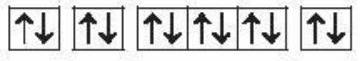
\includegraphics[max width=\textwidth]{2025_10_23_57761e23b8c46a11c3efg-09}
 & $1 s^{2} 2 s^{2} 2 p^{6} 3 s^{2}$ & Kim loại \\
\hline
${ }_{24} \mathrm{Cr}$ & 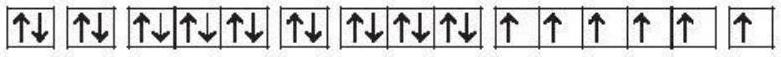
\includegraphics[max width=\textwidth]{2025_10_23_57761e23b8c46a11c3efg-09(1)}
 & $1 s^{2} 2 s^{2} 2 p^{6} 3 s^{2} 3 p^{6} 3 d^{5} 4 s^{1}$ & Kim loại \\
\hline
\end{tabular}
\end{center}

4.14. Cấu hình electron của $Y$ : $1 s^{2} 2 s^{2} 2 p^{6} 3 s^{2} 3 p^{1} \Rightarrow Y$ là kim loại.\\
$Z_{Y}=13 \Rightarrow Z_{X}=10 \Rightarrow$ Cấu hình: $1 s^{2} 2 s^{2} 2 p^{6}$ (loại).\\
$\Rightarrow Z_{X}=15 \Rightarrow C$ ấu hình: $1 s^{2} 2 s^{2} 2 p^{6} 3 s^{2} 3 p^{3} \Rightarrow X$ là phi kim.\\
4.15. $Z=2+8+4=14$.\\
$\Rightarrow$ Cấu hình electron của $X$ là $1 s^{2} 2 s^{2} p^{6} 3 s^{2} 3 p^{2}$.\\
4.16*. Nguyên tử của nguyên tố $X$ có tổng số hạt electron trong các phân lớp $p$ là 7 .\\
$\Rightarrow$ Cấu hình electron của nguyên tử $X$ là: $1 s^{2} 2 s^{2} 2 p^{6} 3 s^{2} 3 p^{1}$.\\
$\Rightarrow Z_{X}=13 \Rightarrow X$ là Al.\\
Số hạt mang điện của một nguyên tử $Y$ nhiều hơn số hạt mang điên của một nguyên tử $X$ là 8 hạt.\\
$\Rightarrow 2 Z_{Y}-2 Z_{X}=8 \Leftrightarrow 2 Z_{Y}-2 \times 13=8$.\\
$\Rightarrow Z_{Y}=17 \Rightarrow \mathrm{Y}$ là Cl .\\
4.17*. Nguyên tố có phân lớp d , có 4 lớp electron nên electron cuối cùng trên phân lớp 3d.\\
Cấu hình electron của nguyên tố này có dạng: $1 s^{2} 2 s^{2} 2 p^{6} 3 s^{2} 3 p^{6} 3 d^{4} 4 s^{2}$.\\
Vậy tổng số electron s và electron p là 20 .\\
4.18*. Số electron tối đa của phân lớp $4 s$ là $4 s^{2} \Rightarrow$ số electron ở phân lớp $3 d$ là $3 d^{1}$.

Cấu hình của nguyên tử $A$ là $1 s^{2} 2 s^{2} 2 p^{6} 3 s^{2} 3 p^{6} 3 d^{1} 4 s^{2}$.\\
4.19*. Cấu hình electron của $A$ và $B$ :

\begin{itemize}
  \item Nguyên tử A có 3 trường hợp:
\end{itemize}

\begin{itemize}
  \item Không có electron ở 3d:\\
$\Rightarrow$ Cấu hình electron: $1 s^{2} 2 s^{2} 2 p^{6} 3 s^{2} 3 p^{6} 4 s^{1} \Rightarrow Z=19$ (potassium).
  \item Có electron ở 3d vì 4s1 chưa bão hoà nên:\\
hoặc 3 d nửa bão hoà: $1 s^{2} 2 s^{2} 2 p^{6} 3 s^{2} 3 p^{6} 3 d^{5} 4 s^{1} \Rightarrow Z=24$ (chromium).\\
hoặc 3 d bão hoà: $1 s^{2} 2 s^{2} 2 p^{6} 3 s^{2} 3 p^{6} 3 d^{10} 4 s^{1} \Rightarrow Z=29$ (copper).
\end{itemize}

\begin{itemize}
  \item Nguyên tố B: $1 s^{2} 2 s^{2} 2 p^{6} 3 s^{2} 3 p^{5}, B$ có $Z=17$ (chlorine).
\end{itemize}

\section*{ÔN TẬP CHƯƠNG 1}
OT1.1. Đáp án A.\\
OT1.2. Đáp án B.\\
OT1.3. Đáp án D.\\
OT1.4. Đáp án D.\\
OT1.5. Đáp án C.\\
OT1.6. $\bar{A}_{\mathrm{Br}}=\frac{79 \times 50,7+81 \times 49,3}{100}=79,99$.\\
OT1.7. \% ${ }_{3}^{7} \mathrm{Li}: \mathrm{x}$\\
$\%{ }_{3}^{6} \mathrm{Li}: 100-\mathrm{x}$\\
$\frac{7 . x+(100-x) .6}{100}=6,94 \Rightarrow x=94\left(\%{ }_{3}^{7} \mathrm{Li}\right) \Rightarrow \%{ }_{3}^{6} \mathrm{Li}=6$.\\
OT1.8.

\begin{itemize}
  \item Điện tích của proton: $1,602 \times 10^{-19} \mathrm{C}$.
  \item Hạt nhân carbon có 6 proton.
  \item Điện tích hạt nhân nguyên tử carbon: $6 \times 1,602 \times 10^{-19}=9,612 \times 10^{-19} \mathrm{C}$.
\end{itemize}

OT1.9*.\\
a) Gọi $\mathrm{P}_{1}, \mathrm{P}_{2}$ lần lượt là số proton trong nguyên tử $\mathrm{M}, \mathrm{X}$. Gọi $\mathrm{N}_{1}, \mathrm{~N}_{2}$ lần lượt là số neutron của hai nguyên tử $M, X$.\\
$\left\{\begin{array}{l}\frac{\mathrm{N}_{1}+\mathrm{P}_{1}}{\mathrm{~N}_{1}+\mathrm{P}_{1}+2 \cdot\left(\mathrm{~N}_{2}+\mathrm{P}_{2}\right)} \cdot 100=46,67 \text { (1) } \\ \mathrm{N}_{1}=\mathrm{P}_{1}+4\end{array}\right.$


\begin{equation*}
\mathrm{N}_{2}=\mathrm{P}_{2} \tag{3}
\end{equation*}



\begin{equation*}
\mathrm{P}_{1}+2 \cdot \mathrm{P}_{2}=58 \tag{4}
\end{equation*}


$\Rightarrow P_{1}=26$ (iron), $N_{1}=30, P_{2}=N_{2}=16$ (sulfur)\\
b) Công thức phân tử $\mathrm{MX}_{2}$ là $\mathrm{FeS}_{2}$.

OT1.10*. Gọi số proton và neutron của M lần lượt là p và n số proton và neutron của X lần lượt là $\mathrm{p}^{\prime}$ và $\mathrm{n}^{\prime}$.

\[
\left\{\begin{array}{l}2 .(2 p+n)+\left(2 p^{\prime}+n^{\prime}\right)=140  \tag{1}\\ \left(2.2 p+2 p^{\prime}\right)-\left(2 n+n^{\prime}\right)=44 \\ (p+n)-\left(p^{\prime}+n^{\prime}\right)=23 \\ (2 p+n)-\left(2 p+n^{\prime}\right)=34\end{array}\right.
\]

$\Rightarrow \mathrm{p}=19$ (potassium); $\mathrm{p}^{\prime}=8$ (oxygen); $\mathrm{n}=20 ; \mathrm{n}^{\prime}=8$\\
Cấu hình electron:\\
$K(Z=19) \quad 1 s^{2} 2 s^{2} 2 p^{6} 3 s^{2} 3 p^{6} 4 s^{1}$\\
$\mathrm{O}(\mathrm{Z}=8) \quad 1 \mathrm{~s}^{2} 2 \mathrm{~s}^{2} 2 \mathrm{p}^{4}$\\
Công thức phân tử hợp chất $\mathrm{M}_{2} \mathrm{X}$ là $\mathrm{K}_{2} \mathrm{O}$.

\section*{Chưong 2. BẢNG TUẨN HOÀN CÁC NGUYÊN TỐ HOÁ HOC}
\section*{Bài 5. CẤU TẠO BẢNG TUẦN HOÀN CÁC NGUYÊN TỐ HOÁ HỌC}
5.1. Đáp án A .\\
5.2. Đáp án C .\\
5.3. Đáp án C .\\
5.4. Đáp án D.\\
5.5. Đáp án B.\\
5.6.\\
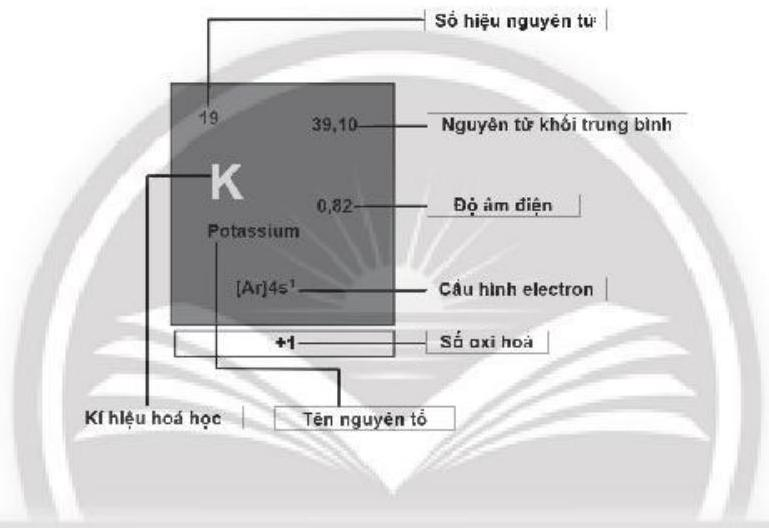
\includegraphics[max width=\textwidth, center]{2025_10_23_57761e23b8c46a11c3efg-11}\\
5.7.

\begin{center}
\begin{tabular}{|c|c|c|c|}
\hline
Họp chất & Khối lượng Fe (g) & Khối lượng O (g) & Tỉ lệ khối lượng O:Fe \\
\hline
FeO & 55,85 & 15,999 & 28,646 \\
\hline
$\mathrm{Fe}_{2} \mathrm{O}_{3}$ & 111,70 & 47,997 & 42,969 \\
\hline
$\mathrm{Fe}_{3} \mathrm{O}_{4}$ & 167,55 & 63,996 & 38,195 \\
\hline
\end{tabular}
\end{center}

5.8. Mổi chu kì gồm các nguyên tố có cùng số lớp electron trong nguyên tử nên số thứ tự của chu kì chính là số lớp electron. Chu kì 3 bắt đầu bằng nguyên tố sodium (kim loại kiềm) và kết thúc bằng khí hiếm argon. Số thứ tự của chu kì bằng 3. Các nguyên tố của chu kì 3 có 3 lớp electron là lớp $K$, lớp $L$ và lớp $M$. Lớp K chỉ có 2 electron được kí hiệu là $1 \mathrm{~s}^{2}$. Lớp L có 8 electron gồm 2 phân lớp đã đầy đủ là $2 s^{2} 2 p^{6}$. Lớp thứ 3 - lớp M gồm 3 phân lớp: $3 \mathrm{~s}, 3 \mathrm{p}$ và 3 d . Với cấu hình electron $3 s^{2} 3 p^{6}$ của khí hiếm argon, chu kì 3 đã kết thúc mặc dù còn lại phân lớp 3d chưa có electron nào. Chu kì 3 chỉ có 8 nguyên tố ứng với số electron trên lớp thứ 3 thay đổi từ 1 đến 8 hay cấu hình electron thay đồi từ $3 s^{1} 3 p^{0}$ (ở nguyên tố sodium) đến $3 s^{2} 3 p^{6}$ (ở nguyên tố argon).\\
5.9.\\
a) $Z=20$; cấu hình electron: $[\mathrm{Ar}] 4 \mathrm{~s}^{2}$; vị trí: ô 20 , chu kì 3 , nhóm IIA (nhóm 2).\\
b) $Z=9$; cấu hình electron: $1 \mathrm{~s}^{2} 2 \mathrm{~s}^{2} 2 \mathrm{p}^{5}$; vị trí: ô 9 , chu kì 2 , nhóm VIIA (nhóm 17).\\
c) $Z=28$; cấu hình electron: $[\mathrm{Ar}] 3 \mathrm{~d}^{8} 4 \mathrm{~s}^{2}$; vị trí: ô 28 , chu kì 4 , nhóm VIIIB (nhóm 10).\\
d) $Z=24$; cấu hình electron: $[\mathrm{Ar}] 3 \mathrm{~d}^{5} 4 \mathrm{~s}^{1}$; vị trí: ô 24 , chu kì 4 , nhóm VIB (nhóm 6).\\
5.10.\\
a) $1 s^{2} 2 s^{2} 2 p^{6} 3 s^{2} 3 p^{1}$. Nguyên tố aluminium.\\
b) $1 s^{2} 2 s^{2} 2 p^{6} 3 s^{2} 3 p^{6} 3 d^{10} 4 s^{1}$. Nguyên tố copper.\\
5.11.\\
a) Gọi số hạt proton, neutron, electron của nguyên tử X là $\mathrm{P}, \mathrm{N}, \mathrm{E}$ và của Y là $P^{\prime}, N^{\prime}, E^{\prime}$.\\
$P=N=E$ và $P^{\prime}=N^{\prime}=E^{\prime} \Rightarrow M_{X}=2 P, M_{Y}=2 P^{\prime}$\\
Trong hợp chất $X Y_{2}, X$ chiếm $50 \%$ về khối lượng, do đó:\\
$M_{X}:\left(2 . M_{Y}\right)=\frac{50}{50}=1 \Rightarrow 2 P:\left(2.2 P^{\prime}\right)=1 \Rightarrow P=2 P^{\prime}$\\
Tồng số proton trong phân tử $X Y_{2}$ là 32 nên $P+2 P^{\prime}=32$\\
$\Rightarrow P=16(S)$ và $P^{\prime}=8(O)$.\\
$\Rightarrow$ Hợp chất cần tìm là $\mathrm{SO}_{2}$.\\
Cấu hình electron của $S: 1 s^{2} 2 s^{2} 2 p^{6} 3 s^{2} 3 p^{4}$ và của $O: 1 s^{2} 2 s^{2} 2 p^{4}$.\\
b) Sulfur ở ô số 16, chu kì 3, nhóm VIA (nhóm 16).

Oxygen ở ô số 8 , chu kì 2 , nhóm VIA (nhóm 16).\\
5.12. a) X và Y đứng kế tiếp trong cùng một chu kì nên số proton của chúng chỉ khác nhau 1 đơn vị.\\
Giá sử $Z_{X}<Z_{Y} \Rightarrow Z_{Y}=Z_{X}+1$\\
Ta có: $Z_{X}+Z_{Y}=Z_{X}+Z_{X}+1=25 \Rightarrow Z_{X}=12$ và $Z_{Y}=13$\\
Cấu hình electron của $X$ : $1 s^{2} 2 s^{2} 2 p^{6} 3 s^{2}$.\\
Cấu hình electron của Y: $1 s^{2} 2 s^{2} 2 p^{6} 3 s^{2} 3 p^{1}$.\\
b) $X$ : ô 12 , chu kì 3 , nhóm IIA (nhóm 2 ) $\Rightarrow X$ là magnesium.

Y: ô 13 , chu kì 3 , nhóm IIIA (nhóm 13 ) $\Rightarrow$ Y là aluminium.\\
5.13. Gọi $Z_{X}, Z_{Y}$ lần lượt là số proton của nguyên tử nguyên tố $X$ và $Y$.

Ta có: $Z_{X}+Z_{Y}=32$ (1)\\
Vì $X, Y$ thuộc cùng nhóm $A$ ở 2 chu kì kế tiếp nhau nên số proton của chúng khác nhau hoặc là $8,18,32$ đơn vị.

Xét 3 trường hợp sau (giả sử $Z_{Y}>Z_{X}$ ):\\
Trường hợp 1: $\mathrm{Z}_{\mathrm{Y}}-\mathrm{Z}_{\mathrm{X}}=8$ (2)\\
Giải (1) và (2) $\Rightarrow Z_{X}=12 ; Z_{Y}=20$.\\
Cấu hình electron của $X$ : $1 s^{2} 2 s^{2} 2 p^{6} 3 s^{2}$.\\
Cấu hình electron của Y: $1 s^{2} 2 s^{2} 2 p^{6} 3 s^{2} 3 p^{6} 4 s^{2}$.\\
Phù hợp với đề bài ( 2 chu kì liên tiếp và ở phân nhóm chính) nên nhận.\\
X là magnesium, Y là calcium.\\
Trường hợp 2: $\mathrm{Z}_{\mathrm{Y}}-\mathrm{Z}_{\mathrm{X}}=18$ (3)\\
Giải (1) và (3) $\Rightarrow Z_{X}=7 ; Z_{Y}=25$.\\
Vậy cấu hình electron của $X$ : $1 s^{2} 2 s^{2} 2 p^{3}$ thuộc chu kì 2 .\\
Cấu hình electron của Y: $1 s^{2} 2 s^{2} 2 p^{6} 3 s^{2} 3 p^{6} 4 s^{2} 3 d^{5}$ thuộc chu kì 4 .\\
Vậy loại trường hợp này vì không thoả mãn điều kiện đề bài.\\
Trường hợp 3: $\mathrm{Z}_{\mathrm{Y}}-\mathrm{Z}_{\mathrm{X}}=32$ (3)\\
Giải (1) và (4) $\Rightarrow Z_{Y}=32 ; Z_{X}=0$ (loại).\\
5.14*. $X$ và $Y$ là 2 nguyên tố thuộc 2 nhóm kế tiếp trong bảng tuần hoàn\\
$\Rightarrow$ Số proton của $X$ và $Y$ hơn kém nhau 1 hoặc 7 hoặc 9 .\\
Trường hợp 1: $\mathrm{P}_{\mathrm{X}}-\mathrm{P}_{\mathrm{Y}}=1 \Rightarrow \mathrm{P}_{\mathrm{X}}=12(\mathrm{Mg}), \mathrm{P}_{\mathrm{Y}}=11(\mathrm{Na})$.\\
Ở trạng thái đơn chất hai nguyên tố này không phản ứng với nhau (loại).\\
Trường hợp 2: $\mathrm{P}_{\mathrm{X}}-\mathrm{P}_{\mathrm{Y}}=7 \Rightarrow \mathrm{P}_{\mathrm{X}}=15(\mathrm{P}), \mathrm{P}_{\mathrm{Y}}=8(\mathrm{O})$.\\
Ở trạng thái đơn chất hai nguyên tố này phản ứng được với nhau (nhận).\\
Trường hợp 3: $P_{X}-P_{Y}=9 \Rightarrow P_{X}=16(S), P_{Y}=7(N)$.\\
Ở trạng thái đơn chất hai nguyên tố này không phản ứng với nhau (loại).\\
Vậy X là phosphorus, Y là oxygen.\\
$5.15^{*} . \mathrm{n}_{\text {NaCI }}=\frac{18,655}{143,5}=0,13(\mathrm{~mol})$.\\
$\overline{\mathrm{M}} \mathrm{Cl}+\mathrm{AgNO}_{3} \rightarrow \overline{\mathrm{M}} \mathrm{NO}_{3}+\mathrm{AgCl}$\\
$0,13 \mathrm{~mol} \quad 0,13 \mathrm{~mol}$\\
$\Rightarrow(\overline{\mathrm{M}}+35,5) \times 0,13=6,645 \Rightarrow \overline{\mathrm{M}}=15,62$\\
2 kim loại kiềm thuộc hai chu kì kế tiếp nhau $\Rightarrow$ lithium ( $\mathrm{M}=7$ ) và sodium $(\mathrm{M}=23)$.

\section*{Bài 6. XU HƯỚNG BIẾN ĐỒI MỘT SỐ TÍNH CHẤT CỦA NGUYÊN TỬ CÁC NGUYÊN TỐ, THÀNH PHẦN VÀ MỘT SỐ TÍNH CHẤT CỦA HỢP CHẤT TRONG MỘT CHU Kİ VÀ NHÓM}
6.1. Đáp án C.\\
6.2. Đáp án D .\\
6.3. Đáp án C.\\
6.4. Đáp án C.\\
6.5. Đáp án C.\\
6.6. Đáp án A .\\
6.7. Đáp án B.\\
6.8. Đáp án D.\\
6.9. Đáp án A.\\
$Z_{X}=4 \Rightarrow X$ thuộc nhóm IIA, chu kì 2 .\\
$Z_{Y}=12 \Rightarrow Y$ thuộc nhóm IIA, chu kì 3.\\
$Z_{Z}=20 \Rightarrow Z$ thuộc nhóm IIA, chu kì 4 .\\
A sai vì nguyên tố nhóm IA mới là các kim loại mạnh nhất trong 1 chu kì.\\
B đúng. $X$ thuộc chu kì $2, Y$ thuộc chu kì $3, Z$ thuộc chu kì 4.\\
$C$ đúng. Trong cùng một nhóm $A$, tính base tăng dần theo chiều tăng dần của điện tích hạt nhân.\\
D đúng. Trong cùng một nhom A , độ âm điện giảm dần theo chiều tăng dần của điện tích hạt nhân.\\
6.10. a) Tính kim loại của nguyên tử một nguyên tố càng mạnh thì tính phi kim của nó càng yếu và ngược lại.\\
b) Độ âm điện của nguyên tử một nguyên tố càng lớn thì tính phi kim của nó càng mạnh.\\
c) Tính phi kim của nguyên tử các nguyên tố biến đổi cùng chiều với độ âm điện của chúng.\\
6.11. He, Kr và Rn đều thuộc nhóm VIIIA. Quả cầu B tượng trưng cho nguyên tử nguyên tố Kr .\\
6.12.

\begin{center}
\begin{tabular}{|c|c|c|c|c|}
\hline
 & Nhóm IA & Nhóm IIIA & Nhóm VA & Nhóm VIIA \\
\hline
Chu kì 2 &  &  &  & F \\
\hline
Chu kì 3 & Na & Al & P & Cl \\
\hline
\end{tabular}
\end{center}

Thứ tự tăng dần độ âm điện: $\mathrm{Na}, \mathrm{Al}, \mathrm{P}, \mathrm{Cl}, \mathrm{F}$.\\
6.13.

\begin{center}
\begin{tabular}{|l|l|l|l|l|l|l|l|}
\hline
 & Nhóm IA & Nhóm IIA & Nhóm IIIA & Nhóm IVA & Nhóm VA & Nhóm VIA & Nhóm VIIA \\
\hline
Chu kì 2 &  &  &  &  &  &  & F \\
\hline
Chu kì 3 & Na & Mg & AI & Si & P & S & Cl \\
\hline
\end{tabular}
\end{center}

Thứ tự giảm dần tính kim loại: $\mathrm{Na}, \mathrm{Mg}, \mathrm{Al}, \mathrm{Si}, \mathrm{P}, \mathrm{S}, \mathrm{Cl}, \mathrm{F}$.\\
6.14.

\begin{center}
\begin{tabular}{ll}
$\mathrm{Na}_{2} \mathrm{O}+\mathrm{H}_{2} \mathrm{O} \rightarrow 2 \mathrm{NaOH}$ & kiềm \\
$\mathrm{CaO}+\mathrm{H}_{2} \mathrm{O} \rightarrow \mathrm{Ca}(\mathrm{OH})_{2}$ & base mạnh \\
$\mathrm{CO}_{2}+\mathrm{H}_{2} \mathrm{O} \rightleftharpoons \mathrm{H}_{2} \mathrm{CO}_{3}$ & acid yếu \\
$\mathrm{N}_{2} \mathrm{O}_{5}+\mathrm{H}_{2} \mathrm{O} \rightarrow 2 \mathrm{HNO}_{3}$ & acid mạnh \\
$\mathrm{SO}_{3}+\mathrm{H}_{2} \mathrm{O} \rightarrow \mathrm{H}_{2} \mathrm{SO}_{4}$ & acid mạnh \\
$\mathrm{Cl}_{2} \mathrm{O}_{7}+\mathrm{H}_{2} \mathrm{O} \rightarrow 2 \mathrm{HClO}_{4}$ & acid mạnh \\
\end{tabular}
\end{center}

$6.15^{*}$.\\
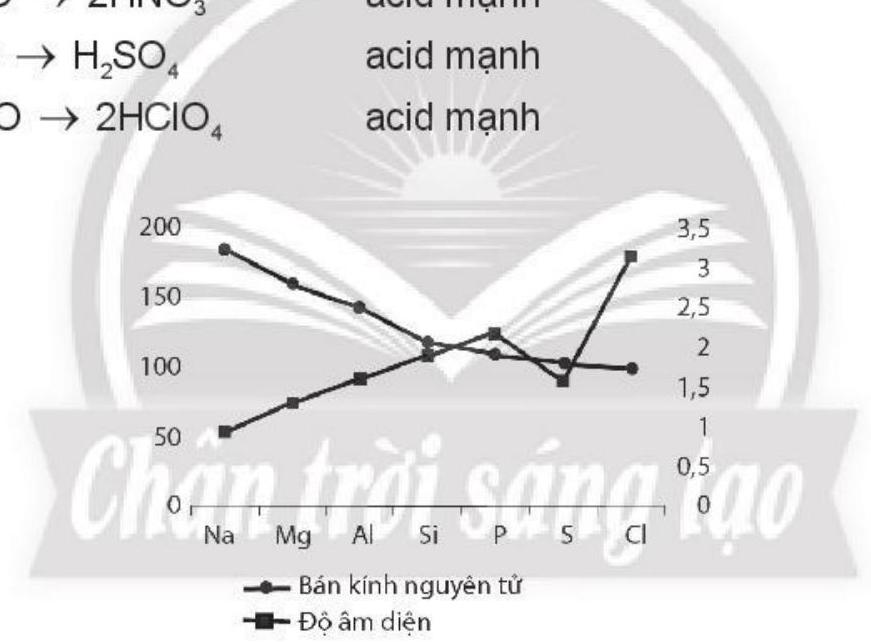
\includegraphics[max width=\textwidth, center]{2025_10_23_57761e23b8c46a11c3efg-15}

\begin{itemize}
  \item Độ âm điện và bán kính nguyên tử của các nguyên tố trong cùng chu kì biến đổi ngược chiều nhau. Bán kính nguyên tử của các nguyên tố trong cùng chu kì giảm dần, còn độ âm điện của các nguyên tố trong cùng chu kì tăng dần.
  \item Trong một chu kì, theo chiều tăng dần của điện tích hạt nhân, lực hút giữa hạt nhân với các electron lớp ngoài cùng cũng tăng theo. Do đó, độ âm điện của nguyên tử các nguyên tố thường tăng dần.
  \item Trong một chu kì, tuy nguyên tử của các nguyên tố có cùng số lớp electron nhưng khi điện tích hạt nhân tăng, lực hút giữa hạt nhân với các electron lớp ngoài cùng cũng tăng theo. Do đó, bán kính nguyên tử của các nguyên tố nói chung giảm khi đi từ đầu chu kì đến cuối chu kì.
\end{itemize}

\section*{Bài 7. ĐỊNH LUẬT TUẦN HOÀN - Ý NGHĨA CỦA BẢNG TUẦN HOÀN CÁC NGUYÊN TỐ HOÁ HỌC}
\section*{7.1. Đáp án B.}
7.2. Đáp án: a) D; b) B; c) D.\\
7.3. Đáp án D.\\
7.4. Đáp án a) D; b) C; c) B.\\
7.5.

\begin{itemize}
  \item Cấu hình electron: $1 s^{2} 2 s^{2} 2 p^{6} 3 s^{2} 3 p^{3}$.
  \item Số electron lớp ngoài cùng: 5.
  \item Phosphorus có tính phi kim.
  \item Công thức oxide cao nhất: $\mathrm{P}_{2} \mathrm{O}_{5}$.
  \item Công thức hợp chất khí với hydrogen: $\mathrm{PH}_{3}$.
  \item Công thức hydroxide cao nhất: $\mathrm{H}_{3} \mathrm{PO}_{4}$.
  \item $\mathrm{P}_{2} \mathrm{O}_{5}$ và $\mathrm{H}_{3} \mathrm{PO}_{4}$ có tính acid.\\
7.6. a) Hợp chất khí với hydrogen của nguyên tố $X$ có công thức $X_{4}$. Oxide cao nhất của X là $\mathrm{XO}_{2}$.\\
$\frac{\mathrm{m}_{\mathrm{o}}}{\mathrm{m}_{\mathrm{xo}_{2}}}=\frac{53,3}{100}$\\
Gọi x là nguyên tử khối của X .\\
$\frac{16 \times 2}{x+16 \times 2}=\frac{53,3}{100} \Rightarrow x=28$\\
b) $X$ thuốc nhóm IVA, nguyên tử khối là 28 . $X$ là silicon ( Si ).\\
7.7. Hợp chất với hydrogen là $\mathrm{RH}_{3} \Rightarrow$ Oxide cao nhất có công thức là: $\mathrm{R}_{2} \mathrm{O}_{5}$.
\end{itemize}

Ta có: $\frac{2 R}{16 \times 5}=\frac{25,93}{74,07}$\\
$\Rightarrow R=14 \Rightarrow R$ là nguyên tố nitrogen (N).\\
7.8. Nhóm VIA nên hợp chất oxide bậc cao là $\mathrm{RO}_{3}$.

Ta có: $\frac{R}{48}=\frac{40}{60} \Rightarrow R=32$ (sulfur).\\
$\Rightarrow$ Công thức oxide cao nhất là: $\mathrm{SO}_{3}$.\\
7.9. Oxide cao nhất của $R$ là $R_{2} O_{5}$ nên $R$ thuộc nhóm VA.\\
$\Rightarrow$ Hợp chất với hydrogen là $\mathrm{RH}_{3}$.\\
Ta có: $\frac{3}{R}=\frac{8,82}{91,18} \Rightarrow R=31(P)$.\\
Hợp chất với hydrogen là $\mathrm{PH}_{3}$.\\
7.10*. Hợp chất với hydrogen có công thức là $\mathrm{RH}_{\mathrm{x}}$.\\
$\Rightarrow$ Hợp chất oxide cao nhất có công thức là $\mathrm{R}_{2} \mathrm{O}_{8-x}$.\\
Ta có:\\
$\left\{\begin{array}{l}\frac{2 R}{16(8-x)}=\frac{27,27}{72,73} \\ \frac{R}{x}=\frac{75}{25}=3\end{array}\right.$\\
$\Rightarrow x=4$ và $R=12$.\\
Vậy R là carbon $\Rightarrow$ oxide cao nhất của R là $\mathrm{CO}_{2}$ và hợp chất khí với hydrogen là $\mathrm{CH}_{4}$.

\section*{ÔN TẬP CHƯƠNG 2}
OT2.1. Đáp án A.\\
OT2.2. Đáp án B.\\
OT2.3. Đáp án B.\\
OT2.4. Đáp án C.\\
OT2.5. Tính phi kim tăng dần: $\mathrm{Al}, \mathrm{Si}, \mathrm{P}$.\\
OT2.6. Tính base giảm dần: $\mathrm{NaOH}, \mathrm{Mg}(\mathrm{OH})_{2}, \mathrm{Al}(\mathrm{OH})_{3}$.\\
OT2.7. Oxide cao nhất của nguyên tố R là $\mathrm{RO}_{3} \Rightarrow$ công thức hợp chất khí với hydrogen của R là $\mathrm{RH}_{2}$.\\
$\frac{\% m_{R}}{\% m_{H}}=\frac{94,12}{5,88}=\frac{M_{R}}{2 M_{H}} \Rightarrow M_{R}=32$.\\
Oxide cao nhất của nguyên tố R là $\mathrm{SO}_{3}$.\\
OT2.8. Hợp chất khí với hydrogen của nguyên tố R là $\mathrm{RH}_{4} \Rightarrow$ Oxide cao nhất của R là $\mathrm{RO}_{2}$.\\
$\frac{\% m_{R}}{\% m_{0}}=\frac{100-53,3}{53,3}=\frac{M_{R}}{2 M_{0}} \Rightarrow M_{R}=28$.\\
Nguyên tố R là silicon (Si).\\
OT2.9*. Gọi số proton của $X, Y$ là $Z_{X}$ và $Z_{Y}$.\\
Nếu $X$ trước $Y$ thì $\left\{\begin{array}{l}Z_{Y}=Z_{X}+1 \\ 2 Z_{X}+Z_{Y}=23\end{array} \Rightarrow Z_{X}=7,3\right.$ (vô lí)\\
Nếu $Y$ trước $X$ thì $\left\{\begin{array}{l}Z_{X}=Z_{Y}+1 \\ 2 Z_{X}+Z_{Y}=23\end{array} \Rightarrow Z_{X}=8\right.$ (oxygen); $Z_{Y}=7$ (nitrogen)\\
Công thức phân tử của $\mathrm{X}_{2} \mathrm{Y}$ là $\mathrm{NO}_{2}$.\\
OT2.10*. Giả sử $X$ đứng trước $Y$.\\
$X, Y$ thuộc cùng nhóm và ở hai chu kì liên tiếp. Do đó, $X$ và $Y$ có thể cách nhau 8, 18 hoặc 32 nguyên tố.\\
$\left\{\begin{array}{l}Z_{X}+Z_{Y}=58 \\ {\left[\begin{array}{l}Z_{Y}=Z_{X}+8 \\ Z_{Y}=Z_{X}+18 \\ Z_{Y}=Z_{X}+32\end{array}\right.}\end{array} \Rightarrow\left[\begin{array}{l}\left\{\begin{array}{l}Z_{X}=25 \\ Z_{Y}=33 \\ Z_{X}=20 \\ Z_{Y}=38\end{array}\right. \\ \left\{\begin{array}{l}Z_{X}=13 \\ Z_{Y}=45\end{array}\right.\end{array}\right.\right.$ (3)\\
Nhận thấy trường hợp (2) thoả yêu cầu đề bài nên $X$ thuộc chu kì 4 , nhóm IIA (calcium) và Y thuộc chu kì 5 , nhóm IIA (strontium).

\section*{Bài 8. QUY TÁC OCTET}
8.1. Đáp án A.\\
8.2. Đáp án C.\\
8.3. Đáp án D.\\
8.4. Đáp án D.\\
8.5. Đáp án D.\\
8.6. Đáp án A . Trong quá trình hình thành phân tử magnesium oxide MgO , nguyên tử magnesium đã đạt được cấu hình bền của khí hiếm gần nhất bằng cách cho đi 2 electron.\\
8.7. Đáp án D. Có 4 nguyên tử trong các phân tử đã cho đạt cấu hình electron bền của khí hiếm neon là $\mathrm{O}, \mathrm{Na}, \mathrm{F}$ và C .\\
8.8. Đáp án D . Trong phân tử $\mathrm{BF}_{3}$, nguyên tử B mới chỉ có 6 electron ở lớp ngoài cùng, chưa đạt được cơ cấu bền của khí hiếm gần nhất.\\
8.9. Nguyên tử oxygen đạt được cấu hình bền của khí hiếm neon trong MgO (chất rắn), $\mathrm{H}_{2} \mathrm{O}$ (chất lỏng) và $\mathrm{O}_{2}$ (chất khí).\\
8.10. Trong phân tử potassium iodide (KI), nguyên tử K và I lần lượt đạt được cơ cấu bền của khí hiếm gần nhất là argon ( Ar ) và xenon ( Xe ).

\section*{Bài 9. LIÊN KẾT ION}
9.1. Đáp án B.\\
9.2. Đáp án D.\\
9.3. Đáp án C.\\
9.4. Đáp án A.\\
9.5. Đáp án B.\\
9.6. Khi cho sodium phản ứng với sulfur, mỗi nguyên tử sodium trong 2 nguyên tử sodium sẽ nhường 1 electron cho nguyên tử sulfur. Kết quả có sự hình thành 2 ion $\mathrm{Na}^{+}$và 1 ion $\mathrm{S}^{2-}$. Các ion này sẽ hút nhau theo lực hút tĩnh điện tạo thành phân tử $\mathrm{Na}_{2} \mathrm{~S}$.\\
9.7. Đáp án C.\\
9.8. Khi cho magnesium tác dụng với chlorine, nguyên tử magnesium sẽ nhường 2 electron cho 2 nguyên tử chlorine. Mỗi nguyên tử chlorine sẽ nhận 1 electron. Kết quả có sự hình thành 1 ion $\mathrm{Mg}^{2+}$ và 2 ion $\mathrm{Cl}^{-}$. Các ion này sẽ hút nhau theo lực hút tĩnh điện tạo thành phân tử $\mathrm{MgCl}_{2}$.\\
9.9. Chú ý $\mathrm{M}_{\mathrm{NaCl}}=58,5 ; \mathrm{M}_{\mathrm{C}_{5} \mathrm{H}_{8} \mathrm{O}, \mathrm{NNa}}=169 ; \mathrm{M}_{\mathrm{C}_{-} \mathrm{H}_{5} \mathrm{O}_{2} \mathrm{Na}}=144$ nên lượng sodium người đó tiêu thụ trong một ngày $=\frac{5 \times 23}{58,5}+\frac{0,5 \times 23}{169}+\frac{0,05 \times 23}{144}=2,042$ gam $=2042 \mathrm{mg}<2300 \mathrm{mg}$.\\
Vậy lượng sodium tiêu thụ này còn nằm trong mức giới hạn cho phép.\\
9.10. Gồm các bước:

\begin{itemize}
  \item Trước hết vẽ một khối lập phương:\\
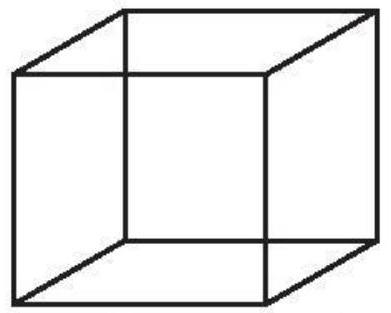
\includegraphics[max width=\textwidth, center]{2025_10_23_57761e23b8c46a11c3efg-20}
  \item Chia khối lập phương đã vẽ thành 8 khối lập phương nhỏ bằng cách nối điểm giữa của mỗi cạnh với điểm giữa của cạnh đối diện và điểm giữa của mỗi mặt với điểm giữa của mặt đối diện:\\
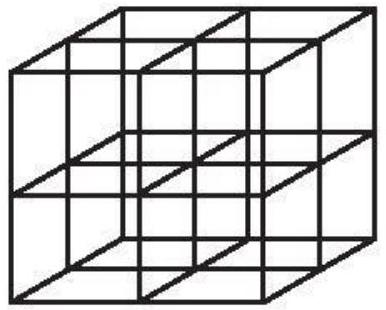
\includegraphics[max width=\textwidth, center]{2025_10_23_57761e23b8c46a11c3efg-21(2)}
  \item Đặt các ion sodium và ion chloride vào các đỉnh của khối lập phương và các điểm giữa của các cạnh cùng các mặt. Chú ý ion chloride có kích thước lớn hơn ion sodium. Tâm của khối lập phương không nhất thiết là ion sodium hay ion chloride, nhưng bắt buộc các ion trái dấu phải luân phiên nhau trong không gian của mạng tinh thể.\\
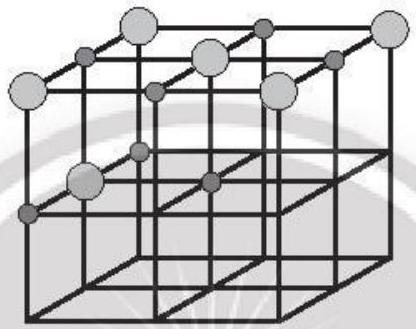
\includegraphics[max width=\textwidth, center]{2025_10_23_57761e23b8c46a11c3efg-21(1)}\\
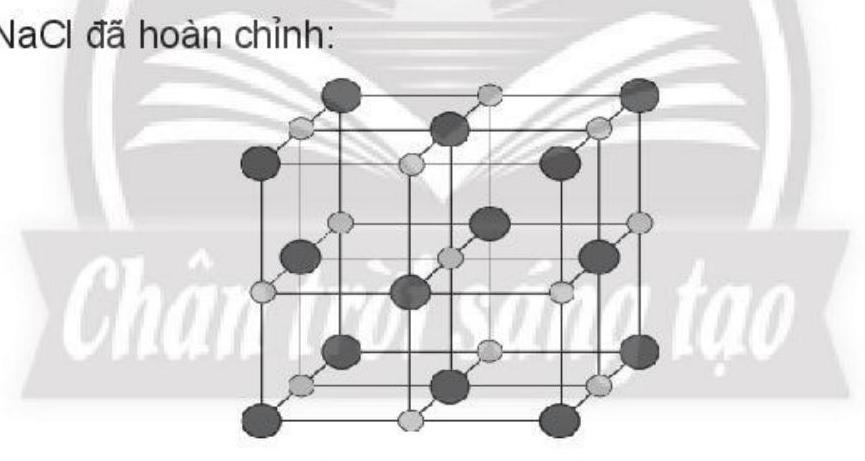
\includegraphics[max width=\textwidth, center]{2025_10_23_57761e23b8c46a11c3efg-21(3)}\\
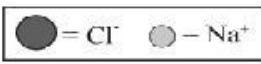
\includegraphics[max width=\textwidth, center]{2025_10_23_57761e23b8c46a11c3efg-21}\\
9.11*. Do hợp chất ion được hình thành bởi các ion có điện tích lớn hơn sẽ tạo ra liên kết bền hơn và các hợp chất ion có độ dài liên kết ngắn hơn sẽ hình thành liên kết bền hơn nên:\\
a) NaCl và $\mathrm{Na}_{2} \mathrm{O}$.
\end{itemize}

Ion $\mathrm{O}^{2-}$ có điện tích lớn hơn ion $\mathrm{Cl}^{-}$, ngoài ra kích thước ion $\mathrm{O}^{2-}$ lại nhỏ hơn ion $\mathrm{Cl}^{-}$nên liên kết trong $\mathrm{Na}_{2} \mathrm{O}$ bền hơn so với NaCl .\\
b) NaCl và NaF .

Tuy các ion $\mathrm{Cl}^{-}$và $\mathrm{F}^{-}$có cùng điện tích, nhưng kích thước ion $\mathrm{F}^{-}$nhỏ hơn ion $\mathrm{Cl}^{-}$nên liên kết trong NaF bền hơn so với NaCl .\\
Thật vậy, hợp chất ion có liên kết bền hơn sẽ có nhiệt độ nóng chảy cao hơn.\\
Nhiệt độ nóng chảy của 3 hợp chất đã cho là:

\begin{center}
\begin{tabular}{|c|c|c|c|}
\hline
 & $\mathrm{Na}_{2} \mathrm{O}$ & $\mathbf{N a F}$ & $\mathbf{N a C l}$ \\
\hline
Nhiệt độ nóng chảy $\left({ }^{\circ} \mathrm{C}\right)$ & 1132 & 993 & 801 \\
\hline
\end{tabular}
\end{center}

9.12*. Nhiệt độ nóng chảy của hợp chất ion là nhiệt độ tại đó có đủ năng lượng dưới dạng nhiệt để phá vỡ lực hút tĩnh điện mạnh giữa các ion và phá vỡ cấu trúc mạng tinh thể, chuyển trạng thái chất từ rắn sang lỏng.

Hợp chất ion có liên kết bền hơn sẽ có nhiệt độ nóng chảy cao hơn.

\begin{itemize}
  \item Do điện tích anion hình thành hợp chất MgO cao hơn so với điện tích anion hình thành hợp chất $\mathrm{MgF}_{2}$, trong khi bán kính anion $\mathrm{O}^{2-}$ và $\mathrm{F}^{-}$là khác biệt không đáng kể ( O và F cùng chu kì 2 ) nên $\mathrm{MgF}_{2}$ phải có nhiệt độ nóng chảy thấp hơn MgO .
  \item Do điện tích cation hình thành hợp chất $\mathrm{MgF}_{2}$ cao hơn điện tích cation hình thành hợp chất NaF , trong khi bán kính cation $\mathrm{Mg}^{2+}$ lại nhỏ hơn cation $\mathrm{Na}^{+}$nên NaF phải có nhiệt độ nóng chảy thấp hơn $\mathrm{MgF}_{2}$.
\end{itemize}

Vậy $X$ là $N a F ; Y$ là $M g F_{2}$ và $Z$ là $M g O$.\\
9.13. Do phân tử NaCl có $\left|q_{1}\right|=\left|q_{2}\right|=1$ đơn vị diện tích; phân tử MgO có $\left|q_{1}\right|=\left|q_{2}\right|=2$ đơn vị diện tích, ngoài ra bán kính cation $\mathrm{Mg}^{2+}$ lại nhỏ hơn bán kính cation $\mathrm{Na}^{+}$ và bán kính anion $\mathrm{O}^{2-}$ cũng lại nhỏ hơn bán kính anion $\mathrm{Cl}^{-}$nên liên kết trong MgO bền hơn nhiều so với trong NaCl , dẫn đến nhiệt độ nóng chảy và nhiệt độ sôi của MgO cao hơn nhiều so với $\mathrm{NaCl}\left(\mathrm{NaCl}\right.$ nóng chảy ở $801^{\circ} \mathrm{C}$ và sôi ở $1413^{\circ} \mathrm{C}$; MgO nóng chảy ở $2850^{\circ} \mathrm{C}$ và sôi ở $3600^{\circ} \mathrm{C}$ ).\\
9.14. Do có sự khác nhau về kích thước và số lượng tương đối của các ion liên kết với nhau nên cấu trúc tinh thể của các hợp chất ion khác nhau sẽ có kích thước và hình dạng khác nhau.\\
9.15. Do các hợp chất ion có cấu trúc tinh thể và lực hút tĩnh điện mạnh nên chúng thường tồn tại ở trạng thái rắn và cứng trong điều kiện thường. Tuy nhiên, chúng lại rất giòn do khi bị tác động bởi một lực, cứ một lớp ion bị khẽ dịch chuyển kéo theo toàn bộ sự sắp xếp sẽ bị xáo trộn do các ion trái dấu tự đẩy nhau, khiến mạng tinh thể bị vỡ (xem hình minh hoạ).\\
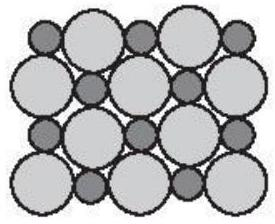
\includegraphics[max width=\textwidth, center]{2025_10_23_57761e23b8c46a11c3efg-23(2)}\\
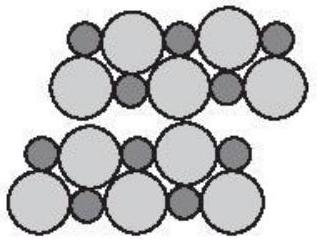
\includegraphics[max width=\textwidth, center]{2025_10_23_57761e23b8c46a11c3efg-23(1)}\\
9.16. Lập phương tâm diện (kí hiệu là FCC: face centered cubic) là cấu trúc lập phương với 8 ion (hoặc nguyên tử) nằm ở các đỉnh hình lập phương và 6 ion (hoặc nguyên tử) khác nằm ở tâm của các mặt của hình lập phương.\\
Tinh thể NaCl được coi là sự đan xen giữa một mạng lập phương tâm diện của các anion với một mạng lập phương tâm diện của các cation (xem hình minh hoạ).\\
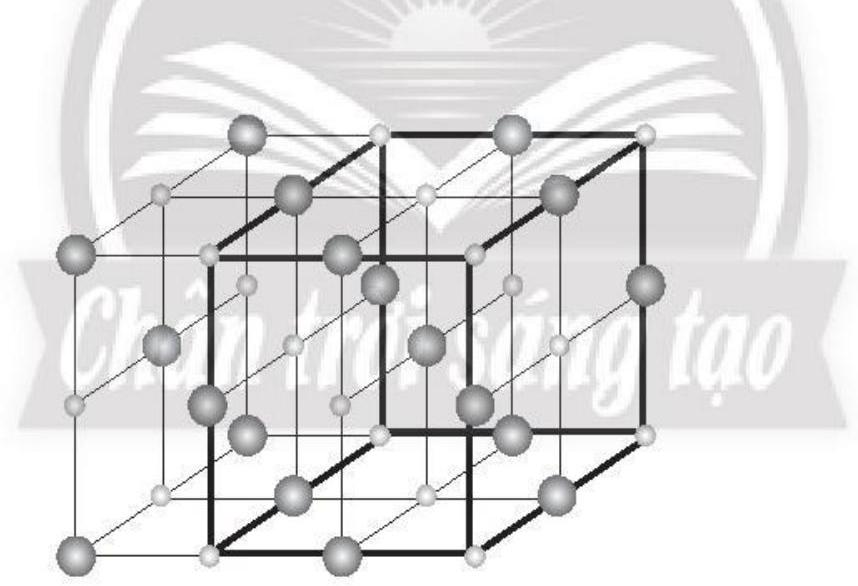
\includegraphics[max width=\textwidth, center]{2025_10_23_57761e23b8c46a11c3efg-23}

\section*{Bài 10. LIÊN KẾT CộNG HOÁ TRỊ}
10.1. Đáp án A .\\
10.2. Đáp án A.\\
10.3. Đáp án A.\\
10.4. Đáp án D . Phân tử $\mathrm{C}_{2} \mathrm{~F}_{6}$ vừa có liên kết cộng hoá trị phân cực giữa các nguyên tử $C$ và nguyên tử $F$, vừa có liên kết cộng hoá trị không phân cực giữa các nguyên tử C với nhau.\\
10.5. Đáp án D . Liên kết $\mathrm{C}-\mathrm{H}$ có hiệu số độ âm điện giữa hai nguyên tử tham gia liên kết là $(3,16-2,96)=0,2<0,4$ nên là liên kết cộng hoá trị không phân cực.\\
10.6. Đáp án B. Do nguyên tử hydrogen có độ âm điện nhỏ nhất nên lực kéo electron về phía nguyên tử nitrogen mạnh nhất ở liên kết $\mathrm{N}-\mathrm{H}$.\\
10.7. Đáp án $B$. Do nguyên tử fluorine có độ âm điện lớn nhất nên liên kết $C-F$ là phân cực nhất.\\
10.8. Đáp án D. Hợp chất KOH chứa cả liên kết cộng hoá trị và liên kết ion.

$$
[K]^{+}[\ddot{0}: \mathbf{H}]
$$

10.9. Đáp án D.\\
10.10. Đáp án C.\\
10.11. Đáp án D.\\
10.12. Đáp án C . Độ bền của liên kết tăng khi độ dài của liên kết giảm.\\
10.13. Nguyên tử nitrogen có 5 electron lớp ngoài cùng, nguyên tử hydrogen có 1 electron lớp ngoài cùng. Trong phân tử $\mathrm{NH}_{3}$, nguyên tử nitrogen góp 3 electron, mỗi nguyên tử hydrogen góp 1 electron hình thành 3 cặp electron chung giữa nguyên tử nitrogen và 3 nguyên tử hydrogen như sau:\\
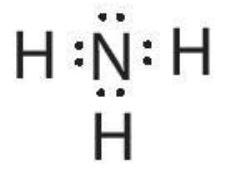
\includegraphics[max width=\textwidth, center]{2025_10_23_57761e23b8c46a11c3efg-24}\\
10.14. Ta có bảng sau:

\begin{center}
\begin{tabular}{|l|l|l|l|}
\hline
Công thức electron & H : $\underset{: H}{: H}$ & 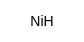
\includegraphics{smile-6d1c1c6c59a45ae1630c20f8dcf641d7b660278c} & :ö:: C::ö \\
\hline
Công thức Lewis & 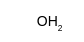
\includegraphics{smile-d9bb0c9bb3eef87aee33bd96641c3201ad545603} & 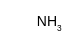
\includegraphics{smile-d0f8f18108d8de41d9548b849ef64c0f13afc857} & 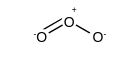
\includegraphics{smile-ce2ef27ef5d4e8de631ee9eddc4f89c57c2f7b07} \\
\hline
Công thức cấu tạo & $\mathrm{H}-\mathrm{O}-\mathrm{H}$ & 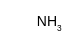
\includegraphics{smile-549ce04ec05374711c5e3bd7129df72db9315ede} & $\mathrm{O}=\mathrm{C}=\mathrm{O}$ \\
\hline
\end{tabular}
\end{center}

10.15. Trong phân tử ozone có liên kết cho - nhận nên công thức Lewis và công thức cấu tạo của ozone lần lượt là:\\
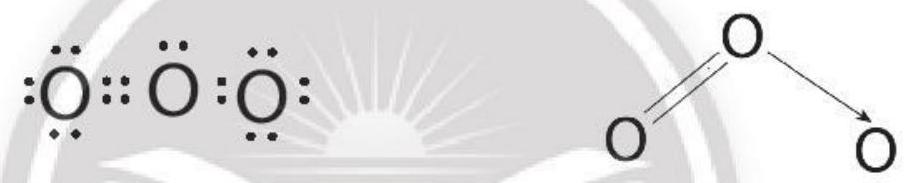
\includegraphics[max width=\textwidth, center]{2025_10_23_57761e23b8c46a11c3efg-25(1)}\\
10.16. Sự hình thành liên kết cho - nhận trong ion ammonium từ ammonia và proton ( $\mathrm{H}^{+}$):\\
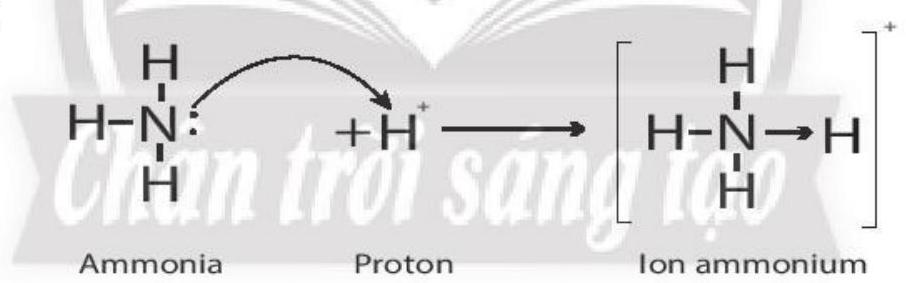
\includegraphics[max width=\textwidth, center]{2025_10_23_57761e23b8c46a11c3efg-25}\\
10.17.

\begin{itemize}
  \item Giống nhau: Liên kết ion và liên kết cộng hoá trị đều là nguyên nhân giúp các nguyên tử hình thành nên phân tử, trong đó các nguyên tử trong phân tử đều đạt được cơ cấu bền vững của khí hiếm gần nhất.\\
Ví dụ liên kết ion là nguyên nhân hình thành liên kết giữa nguyên tử sodium và nguyên tử chlorine tạo nên phân tử sodium chloride. Liên kết cộng hoá trị là nguyên nhân hình thành liên kết giữa hai nguyên tử chlorine tạo nên phân tử chlorine. Trong các phân tử trên, các nguyên tử sodium và chlorine đều đạt được cơ cấu bền vững của khí hiếm neon và argon.
  \item Khác nhau:
\end{itemize}

\begin{center}
\begin{tabular}{|l|l|l|}
\hline
Loại liên kết & Liên kết ion & Liên kết cộng hoá trị \\
\hline
Bản chất & Là lực hút tĩnh điện giữa các ion trái dấu. & Là sự tạo thành các cặp eletron chung. \\
\hline
\begin{tabular}{l}
Điều kiện \\
liên kết \\
\end{tabular} & Xuất hiện giữa nguyên tử của các nguyên tố khác biệt nhau về bản chất hoá học. & Xuất hiện giữa nguyên tử của các nguyên tố giống nhau hay gần giống nhau về bản chất hoá học. \\
\hline
Ví dụ & Sodium $(\mathrm{Na})$ và chlorine $(\mathrm{Cl})$ là nguyên tử của các nguyên tố khác nhau về bản chất hoá học. & Hai nguyên tử chlorine $(\mathrm{Cl})$ trong phân tử chlorine $\left(\mathrm{Cl}_{2}\right)$ giống nhau về bản chất hoá học. \\
\hline
\end{tabular}
\end{center}

10.18. a) Công thức Lewis và công thức cấu tạo của hydrogen sulfide là:

$$
H: \ddot{S}: H \quad H-S-H
$$

b) Nồng độ ppm (parts per million - thành phần phần triệu) của $\mathrm{H}_{2} \mathrm{~S}$ trong không khí là số lít khí $\mathrm{H}_{2} \mathrm{~S}$ có trong 1000000 L không khí.

Ví dụ nếu trong 1000 L không khí có lẫn $0,1 \mathrm{~L} \mathrm{H}_{2} \mathrm{~S}$\\
thì trong 1000000 L không khí có $\frac{1000000 \times 0,1}{1000}=100 \mathrm{~L} \mathrm{H}_{2} \mathrm{~S}$.\\
Ta nói nồng độ ppm của $\mathrm{H}_{2} \mathrm{~S}$ trong không khí là 100 ppm .\\
c) Thể tích không khí $=$ thể tích gian phòng $=3 \times 4 \times 6=72 \mathrm{~m}^{3}$.

Thể tích của 10 gam $\mathrm{H}_{2} \mathrm{~S}=\frac{24,79 \times 10}{34}=7,3 \mathrm{~L}$.\\
Trong $72 \mathrm{~m}^{3}$ tức trong 72000 L không khí có $7,3 \mathrm{~L} \mathrm{H}_{2} \mathrm{~S}$ nên trong 1000000 L không khí có $\frac{1000000 \times 7,3}{72000} \approx 101,38 \mathrm{~L} \mathrm{H}_{2} \mathrm{~S}$. Vậy nồng độ $\mathrm{H}_{2} \mathrm{~S}$ trong gian phòng là 101,38 ppm nên gây kích thích màng phổi.\\
10.19. Sơ đồ biểu diễn sự xen phủ giữa orbital 1 s của nguyên tử hydrogen và orbital 3 p của nguyên tử chlorine trong sự hình thành liên kết $\sigma$ trong phân tử hydrogen chloride ( HCl ):\\
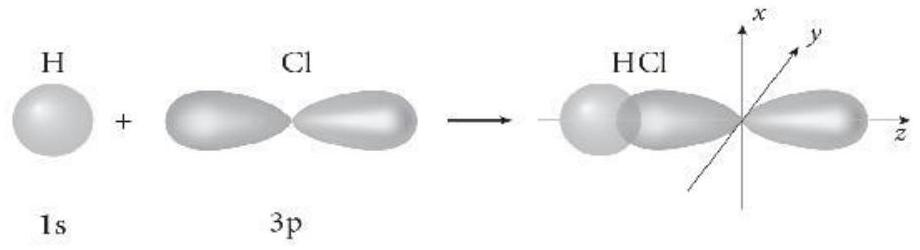
\includegraphics[max width=\textwidth, center]{2025_10_23_57761e23b8c46a11c3efg-26}\\
10.20. Dựa theo kết quả trong bảng sau:

\begin{center}
\begin{tabular}{|c|c|c|c|}
\hline
 & $\mathrm{C}-\mathrm{C}$ & $\mathrm{C}=\mathrm{C}$ & $\mathrm{C} \equiv \mathrm{C}$ \\
\hline
Độ dài liên kết $(\AA)$ & $\stackrel{\circ}{\mathrm{A}})$ & 1,54 & 1,34 \\
\hline
Năng lượng liên kết $(\mathrm{kJ} / \mathrm{mol})$ & 347 & 614 & 1,20 \\
\hline
\end{tabular}
\end{center}

Ta thấy độ dài liên kết và năng lượng liên kết biến thiên tỉ lệ nghịch với nhau: Năng lượng liên kết lớn thì độ dài liên kết ngắn (và ngược lại).\\
10.21. Tuy có độ âm điện xấp xỉ nhau nhưng phân tử nitrogen có liên kết ba ( $\mathrm{N} \equiv \mathrm{N}$ ), còn phân tử chlorine chỉ có liên kết đơn $(\mathrm{Cl}-\mathrm{Cl})$ nên phân tử nitrogen có năng lượng liên kết ( $945 \mathrm{~kJ} / \mathrm{mol}$ ) lớn hơn nhiều so với phân tử chlorine ( $243 \mathrm{~kJ} / \mathrm{mol}$ ), dẫn đến phải tiêu tốn năng lượng nhiều hơn để phá vỡ liên kết trong phân tử nitrogen so với trong phân tử chlorine. Vì vậy ở điều kiện thường, nitrogen kém hoạt động hơn nhiều so với chlorine.\\
10.22. Trên biểu đồ, năng lượng tối thiểu đại diện cho độ bền liên kết và khoảng cách $\mathrm{r}_{\mathrm{o}}$ tại mức năng lượng tối thiểu gọi là độ dài liên kết. Do đó phân tử $\mathrm{H}_{2}$ có năng lượng liên kết là $432 \mathrm{~kJ} / \mathrm{mol}$ và có độ dài liên kết $\mathrm{H}-\mathrm{H}$ là 74 pm .\\
10.23. Sodium chloride là hợp chất ion nên chỉ tan trong dung môi phân cực là nước, không tan trong dung môi không phân cực là dầu hoả.\\
10.24. Benzene $\left(\mathrm{C}_{6} \mathrm{H}_{6}\right)$ là hợp chất không phân cực nên benzene không tan trong dung môi phân cực (nước) mà tan tốt trong các dung môi không phân cực như tetrachloromethane $\left(\mathrm{CCl}_{4}\right)$, hexane $\left(\mathrm{C}_{6} \mathrm{H}_{14}\right), \ldots$\\
10.25*. Ba phân tử đầu đều là các phân tử phân cực, do tổng moment lưỡng cực không triệt tiêu. Hai phân tử sau đều là các phân tử không phân cực do tổng moment lưỡng cực triệt tiêu.\\
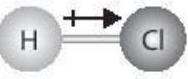
\includegraphics[max width=\textwidth, center]{2025_10_23_57761e23b8c46a11c3efg-27}\\
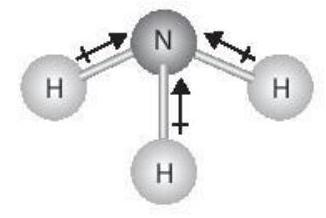
\includegraphics[max width=\textwidth, center]{2025_10_23_57761e23b8c46a11c3efg-27(4)}\\
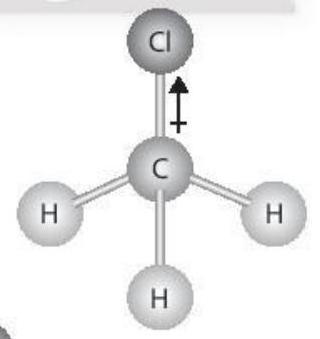
\includegraphics[max width=\textwidth, center]{2025_10_23_57761e23b8c46a11c3efg-27(2)}\\
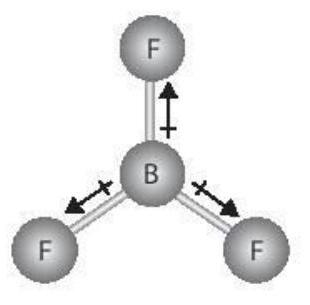
\includegraphics[max width=\textwidth, center]{2025_10_23_57761e23b8c46a11c3efg-27(1)}\\
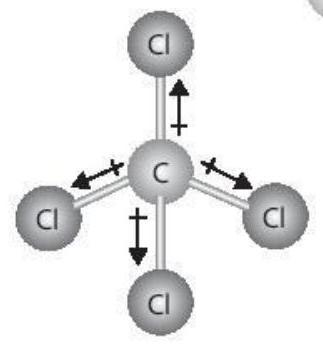
\includegraphics[max width=\textwidth, center]{2025_10_23_57761e23b8c46a11c3efg-27(3)}\\
10.26*.\\
a) Phân tử $\mathrm{CO}_{2}$ có dạng đường thẳng nên $\mathrm{CO}_{2}$ là phân tử không phân cực; Phân tử $\mathrm{SO}_{2}$ có dạng góc nên $\mathrm{SO}_{2}$ là phân tử phân cực. Như vậy $\mathrm{CO}_{2}$ là phân tử không phân cực nên $\mathrm{CO}_{2}$ tan kém trong nước là dung môi phân cực, trái với $\mathrm{SO}_{2}$ là phân tử phân cực nên $\mathrm{SO}_{2}$ tan được nhiều hơn trong nước là dung môi phân cực.\\
b) Trên đồ thị, độ tan của $\mathrm{CO}_{2}$ trong nước giảm khi nhiệt độ tăng.\\
c) Nước giải khát có gas là nước giải khát được nạp khí $\mathrm{CO}_{2}$. Trong sản xuất, người ta nạp $\mathrm{CO}_{2}$ vào nước giải khát ở nhiệt độ thấp và áp suất cao để $\mathrm{CO}_{2}$ tan được nhiều hơn. Khi uống nước giải khát có gas, nhiệt độ cao trong dạ dày làm $\mathrm{CO}_{2}$ nhanh chóng theo đường miệng thoát ra ngoài, mang đi bớt một nhiệt lượng trong cơ thể làm cho người uống có cảm giác mát mẻ, dễ chịu.\\
Do $\mathrm{CO}_{2}$ tan tốt trong nước ở nhiệt độ thấp hơn nên để giữ lại lượng $\mathrm{CO}_{2}$ trong nước, người ta thường ướp lạnh các loại nước giải khát trước khi sử dụng.\\
d) Oxygen là phân tử không phân cực nên khả năng tan trong nước là dung môi phân cực cũng kém. Giống như độ hoà tan của carbon dioxide trong nước, độ hoà tan của oxygen giảm khi nhiệt độ tăng. Do đó vào mùa lạnh, cá có thể thở dễ dàng bằng lượng oxygen tan trong nước, còn mùa hè lượng oxygen tan trong nước it hơn nên chúng phải thường ngoi lên mặt nước đề thở.

\section*{Bài 11. LIÊN KẾT HYDROGEN VÀ TƯƠNG TÁC VAN DER WAALS}
11.1. Đáp án D.\\
11.2. Đáp án D.\\
11.3. Đáp án $A$.\\
11.4. Đáp án A . Liên kết hydrogen liên phân tử là lực hút tĩnh điện giữa nguyên tử H (thường trong các liên kết $\mathrm{H}-\mathrm{F} ; \mathrm{H}-\mathrm{N} ; \mathrm{H}-\mathrm{O}$ ở phân tử này) với một trong các nguyên tử có độ âm điện mạnh (thường là $\mathrm{N} ; \mathrm{O} ; \mathrm{F}$ ) ở một phân tử khác.\\
11.5. Đáp án $B$. Liên kết hydrogen nội phân tử là lực hút tĩnh điện giữa nguyên tử $H$ ( thường trong các liên kết $\mathrm{H}-\mathrm{F} ; \mathrm{H}-\mathrm{N} ; \mathrm{H}-\mathrm{O}$ ) ở một phân tử với một trong các nguyên tử có độ âm điện mạnh (thường là $\mathrm{N} ; \mathrm{O} ; \mathrm{F}$ ) ở ngay chính phân tử đó.\\
11.6. Đáp án B. Tương tác van der Waals xuất hiện là do sự hình thành các lưỡng cực tạm thời cũng như các lưỡng cực cảm ứng. Các lưỡng cực tạm thời xuất hiện là do sự chuyển động của các electron trong phân tử, đó là lúc electron tập trung về một phía trong phân tử.\\
11.7. Đáp án B. Do có khối lượng phân tử lớn nhất nên tương tác van der Waals giữa các phân tử Xe là lớn nhất, dẫn đến khí hiếm Xe có nhiệt độ sôi cao nhất.\\
11.8. a)

\begin{figure}[h]
\begin{center}
  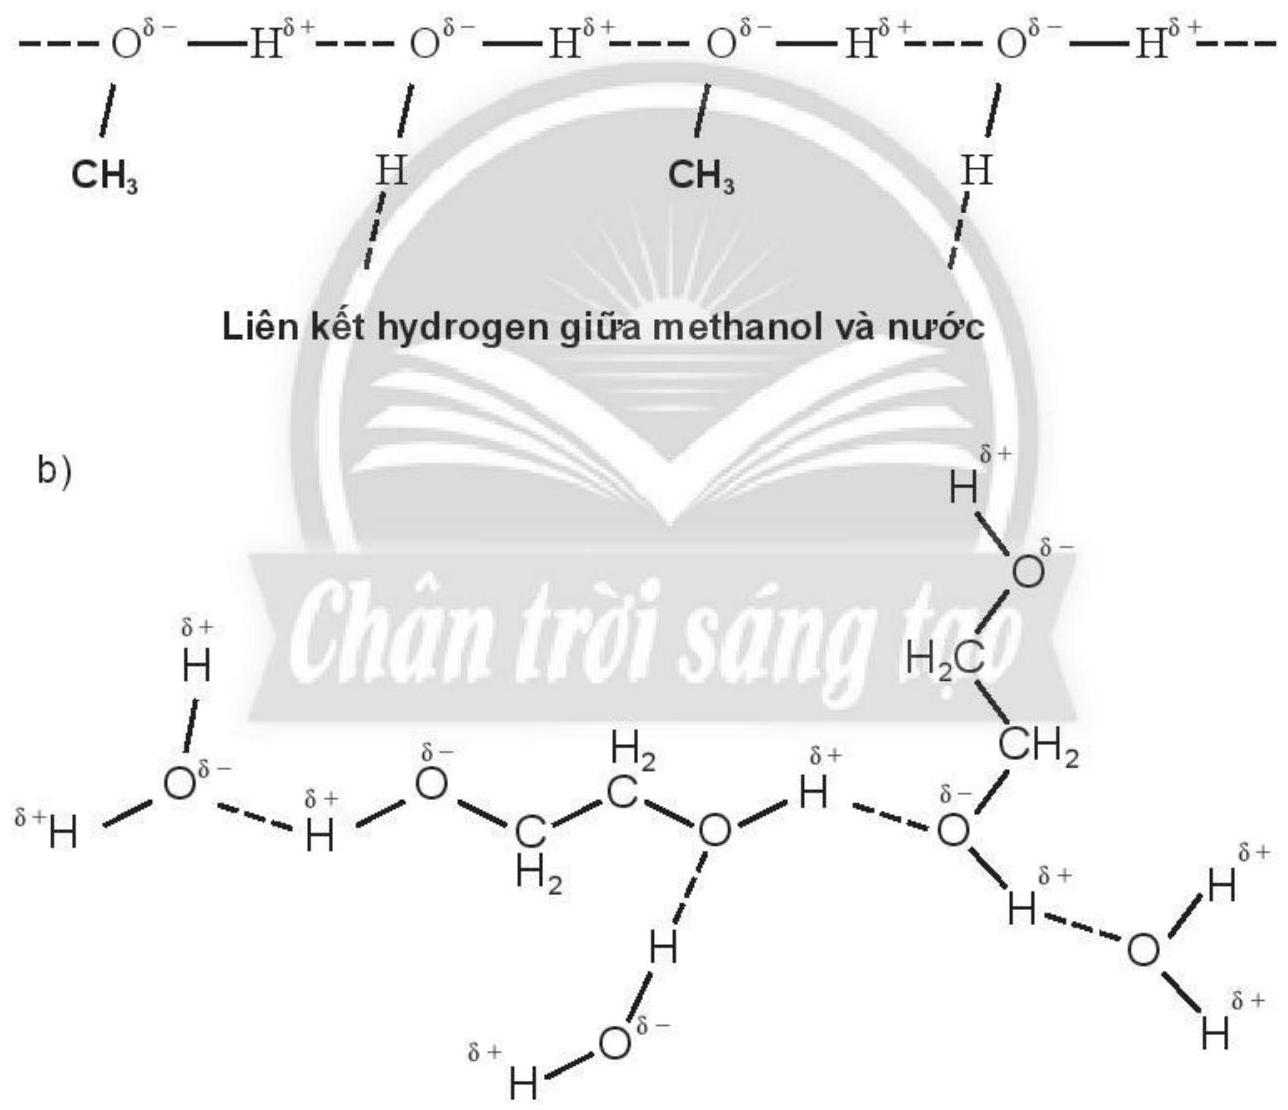
\includegraphics[width=\textwidth]{2025_10_23_57761e23b8c46a11c3efg-29}
\captionsetup{labelformat=empty}
\caption{Liên kết hydrogen giữa ethylene glycol và nước}
\end{center}
\end{figure}

Do methanol và ethylene glycol tạo được liên kết hydrogen với nước nên methanol và ethylene glycol đều tan vô hạn trong nước.\\
11.9.\\
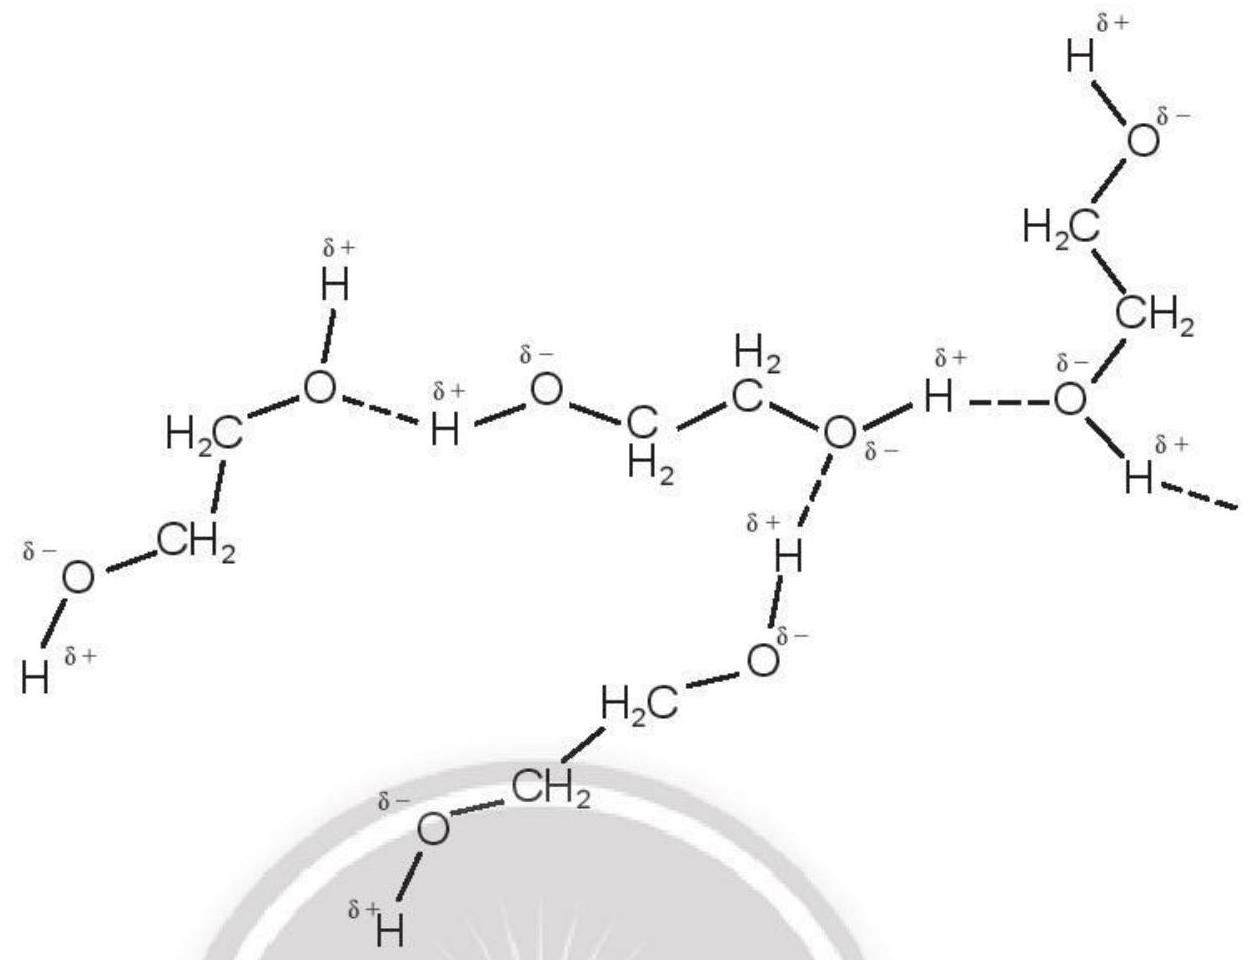
\includegraphics[max width=\textwidth, center]{2025_10_23_57761e23b8c46a11c3efg-30}\\
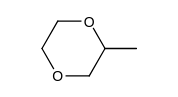
\includegraphics{smile-d578bdcc71cfd9983deb737ed51ed8d36c1167dd}

Liên kết hydrogen nội phân tử ethylene glycol\\
11.10. Tương tác van der Waals và liên kết ion đều là các lực hút tĩnh điện. Tuy nhiên, tương tác van der Waals là lực hút tĩnh điện giữa các phân tử trung hoà nên yếu hơn nhiều so với liên kết ion là lực hút tĩnh điện giữa các ion trái dấu.\\
11.11. Oxygen có khối lượng phân tử cao hơn nitrogen, do đó tương tác van der Waals giữa các phân tử oxygen mạnh hơn so với nitrogen. Kết quả oxygen lỏng có nhiệt độ sôi cao hơn nitrogen lỏng. Thật vậy, oxygen lỏng sôi ở $-183^{\circ} \mathrm{C}$, trong khi nitrogen lỏng sôi ở $-195,8^{\circ} \mathrm{C}$.\\
11.12. Phân tử có kích thước lớn thường đi đôi với nhiều electron. Chính vì vậy khả năng tạo các lưỡng cực tức thời và lưỡng cực cảm ứng của các phân tử có kích thước lớn cũng nhiều hơn, từ đó tương tác van der Waals giữa các phân tử lớn cũng mạnh hơn, nên các phân tử có kích thước lớn "dính" với nhau hơn so với các phân tử có kích thước nhỏ.\\
11.13*. Khi đi từ $F_{2}$ đến $I_{2}$, do khối lượng phân tử các halogen tăng dần làm tương tác van der Waals giữa các phân tử halogen cũng tăng dần, kết quả các phân tử halogen "dính" với nhau chặt hơn, nên fluorine và chlorine ở trạng thái khí, còn bromine ở trạng thái lỏng và iodine ở trạng thái rắn.\\
11.14*.\\
a) Các nguyên tố đầu tiên trong mỗi nhóm VA, VIA, VIIA ( $\mathrm{N}, \mathrm{O}, \mathrm{F}$ ) có kích thước nhỏ và có độ âm điện lớn, kết quả trong các hợp chất $\mathrm{NH}_{3} ; \mathrm{H}_{2} \mathrm{O} ; \mathrm{HF}$ xuất hiện liên kết hydrogen liên phân tử làm các hợp chất này có nhiệt độ sôi cao bất thường so với các hợp chất còn lại trong mỗi nhóm.\\
b) Hợp chất với hydrogen của các nguyên tố còn lại trong mỗi nhóm có nhiệt độ sôi tăng dần khi khối Iượng phân tử của chúng tăng. Vì khi khối lượng phân tử tăng, tương tác van der Waals giữa các phân tử trong hợp chất cũng tăng làm các phân tử "dinh" với nhau chặt hơn, dẫn đến nhiệt độ sôi của chúng dần cao hơn.\\
11.15*. Hai hợp chất đã cho có cùng công thức phân tử, tức cùng khối lượng phân tử. Tuy nhiên phân tử neopentane có dạng hình cầu nên diện tích bề mặt tiếp xúc giữa các phân tử neopentane nhỏ hơn so với các phân tử pentane. Kết quả các phân tử pentane "dính" với nhau hơn so với các phân tử neopentane nên nhiệt độ nóng chảy và nhiệt độ sôi của pentane $\left(-130^{\circ} \mathrm{C}\right.$ và $36,0^{\circ} \mathrm{C}$ ), cao hơn so với neopentane ( $-16,6^{\circ} \mathrm{C}$ và $9,5^{\circ} \mathrm{C}$ ).\\
11.16*. $\mathrm{CHCl}_{3}$ là một phân tử phân cực, trong khi $\mathrm{CCl}_{4}$ là một phân tử không phân cực. Như vậy, $\mathrm{CHCl}_{3}$ đáng lí phải có nhiệt độ sôi cao hơn $\mathrm{CCl}_{4}$. Tuy nhiên thực tế $\mathrm{CCl}_{4}$ lại có nhiệt độ sôi cao là $76,8^{\circ} \mathrm{C}$, cao hơn so với $\mathrm{CHCl}_{3}$ là $61,2^{\circ} \mathrm{C}$. Điều này là do phân tử $\mathrm{CCl}_{4}$ có kích thước lớn hơn $\mathrm{CHCl}_{3}$ nên có số electron cũng nhiều hơn $\mathrm{CHCl}_{3}$, do đó tương tác van der Waals giữa các phân tử $\mathrm{CCl}_{4}$ mạnh hơn so với $\mathrm{CHCl}_{3}$ làm cho $\mathrm{CCl}_{4}$ có nhiệt độ sôi cao hơn $\mathrm{CHCl}_{3}$.

\section*{ÔN TẬP CHƯƠNG 3}
OT3.1. Đáp án D. Ion $\mathrm{Li}^{+}$có cấu hình electron của khí hiếm helium.\\
OT3.2. Đáp án A . Trong sự hình thành phân tử lithium fluoride (LiF), ion lithium và ion fluoride đã lần lượt đạt được cấu hình electron bền của các khí hiếm helium và neon.

OT3.3. Đáp án B. Phân tử $\mathrm{BaCl}_{2}$ và $\mathrm{Na}_{2} \mathrm{O}$ có sự liên kết giữa kim loại điển hình và phi kim điển hình nên chúng có liên kết ion.

OT3.4. Trong số các phân tử $\mathrm{Cl}_{2}, \mathrm{O}_{2}, \mathrm{CCl}_{4}, \mathrm{CO}_{2}$ và $\mathrm{SO}_{2}$, các phân tử $\mathrm{Cl}_{2}$ và $\mathrm{O}_{2}$ không hình thành moment lưỡng cực, còn phân tử $\mathrm{CCl}_{4}$ có dạng tứ diện đều và phân tử $\mathrm{CO}_{2}$ có dạng đường thẳng nên phân tử $\mathrm{CCl}_{4}$ và phân tử $\mathrm{CO}_{2}$ có tổng moment lưỡng cực bằng không. Vậy các phân tử $\mathrm{Cl}_{2}, \mathrm{O}_{2}, \mathrm{CCl}_{4}$ và $\mathrm{CO}_{2}$ đều là phân tử không cực. Phân tử $\mathrm{SO}_{2} \mathrm{co}$ dạng góc nên là phân tử có cực.

OT3.5. Phân tử NaF và MgO có cùng 20 electron và khoảng cách giữa các hạt nhân là tương tự nhau ( 235 pm và 215 pm), tuy nhiên nhiệt độ nóng chảy của MgO cao hơn nhiều so với NaF , đó là do các ion magnesium và oxide mang điện tích lần lượt +2 và -2 nên có lực hút tĩnh điện mạnh hơn nhiều so với các ion sodium và fluoride chỉ mang điện tích lần lượt là +1 và -1 .

OT3.6. Lực hút tĩnh điện mạnh giữa các ion âm và ion dương làm cho LiF và NaCl đều có nhiệt độ nóng chảy và nhiệt độ sôi cao. Do các ion lithium và sodium đều mang điện tích +1 , các ion fluoride và chloride đều mang điện tích -1 nên lực hút tĩnh điện ở đây phụ thuộc vào khoảng cách giữa các ion trong mỗi phân tử. Nếu các ion càng nhỏ, chúng càng gần nhau hơn dẫn đến lực hút tĩnh điện lớn hơn. Do kích thước ion $\mathrm{Na}^{+}$Iớn hơn ion $\mathrm{Li}^{+}$, kích thước ion $\mathrm{Cl}^{-}$Iớn hơn ion $\mathrm{F}^{-}$nên lực hút tĩnh điện giữa các ion trong phân tử LiF lớn hơn trong phân tử NaCl làm nhiệt độ sôi và nhiệt độ nóng chảy của NaCl cao hơn LiF.\\
Bảng số liệu tham khảo:

\begin{center}
\begin{tabular}{|l|l|l|}
\hline
 & LiF ( ${ }^{\circ} \mathrm{C}$ ) & $\mathrm{NaCl}\left({ }^{\circ} \mathrm{C}\right)$ \\
\hline
Nhiệt độ nóng chảy & 848,2 & 800,7 \\
\hline
Nhiệt độ sôi & 1680,0 & 1465,0 \\
\hline
\end{tabular}
\end{center}

OT3.7. Ta có công thức của $\mathrm{Na}_{2} \mathrm{O}_{2}$ :

$$
\mathrm{Na} \text { [ }[\ddot{0}: \ddot{0}: \ddot{0}:]^{2-} \mathrm{Na}^{+}
$$

Công thức này cho thấy trong phân tử $\mathrm{Na}_{2} \mathrm{O}_{2}$, liên kết giữa 2 nguyên tử oxygen là liên kết cộng hoá trị không phân cực. Ngoài ra, mỗi nguyên tử sodium nhường 1 electron cho mỗi nguyên tử oxygen, hình thành nên các ion $\mathrm{O}_{2}^{2-}$ và 2 ion $\mathrm{Na}^{+}$. Những ion này hút nhau bằng lực hút tĩnh điện tạo nên phân tử $\mathrm{Na}_{2} \mathrm{O}_{2}$.

OT3.8. Liên kết hydrogen không phải là sự xen phủ giữa các orbital, mà chỉ là lực hút tĩnh điện giữa nguyên tử hydrogen mang một phần điện tích âm đã liên kết với một nguyên tử có độ âm điện lớn (thường là $\mathrm{N}, \mathrm{O}, \mathrm{F}$ ) với một nguyên tử có độ âm điện lớn khác (thường là $\mathrm{N}, \mathrm{O}, \mathrm{F}$ ).\\
Ví dụ ta có liên kết hydrogen giữa các phân tử $\mathrm{H}_{2} \mathrm{O}$ như sau:

OT3.9.\\
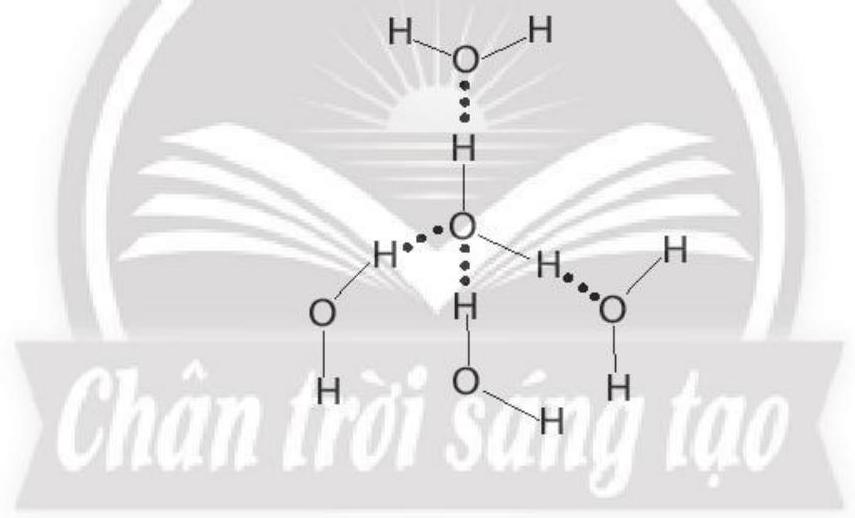
\includegraphics[max width=\textwidth, center]{2025_10_23_57761e23b8c46a11c3efg-33}\\
a) Chiều dài liên kết tỉ lệ nghịch với năng lượng liên kết giữa các nguyên tử carbon trong các hydrocarbon đã cho .\\
b) Giá trị các năng lượng liên kết tăng theo thứ tự $\mathrm{C}-\mathrm{C} ; \mathrm{C}=\mathrm{C} ; \mathrm{C} \equiv \mathrm{C}$ do độ bền các liên kết tăng dần theo thứ tự $\mathrm{C}-\mathrm{C} ; \mathrm{C}=\mathrm{C} ; \mathrm{C} \equiv \mathrm{C}$

OT3.10. Ethane $\left(\mathrm{C}_{2} \mathrm{H}_{6}\right)$ và fluoromethane $\left(\mathrm{CH}_{3} \mathrm{~F}\right)$ có kích thước tương đương nhau và đều có 18 electron. Như vậy tương tác van der Waals giữa các phân tử trong mỗi hợp chất là tương tự nhau dẫn đến nhiệt độ sôi của chúng lẽ ra phải tương tự nhau. Tuy nhiên, $\mathrm{C}_{2} \mathrm{H}_{6}$ là phân tử không phân cực, còn $\mathrm{CH}_{3} \mathrm{~F}$ là phân tử phân cực nên nhiệt độ sôi của $\mathrm{CH}_{3} \mathrm{~F}$ cao hơn $\mathrm{C}_{2} \mathrm{H}_{6}$ khoảng hơn $10^{\circ}$.

\section*{Chưong 4. PHẢN ÚNG OXI HOÁ - KHƯ}
\section*{BÀI 12. PHẢN ỨNG OXI HOÁ - KHỬ VÀ ỨNG DỤNG TRONG CUỘC SỐNG}
12.1. Đáp án B.\\
12.2. Đáp án B.\\
12.3. Đáp án D.\\
12.4. Đáp án B.\\
12.5. Đáp án $C$.\\
12.6. Đáp án B.\\
12.7. Đáp án D.\\
12.8. Đáp án B.\\
12.9. Đáp án C.\\
12.10. Đáp án B.\\
12.11. Số oxi hoá của các nguyên tố trong các chất và ion theo thứ tự:\\
a) $\mathrm{Fe}: 0 ; \mathrm{N}_{2}: 0 ; \mathrm{SO}_{3}:+6,-2 ; \mathrm{H}_{2} \mathrm{SO}_{4}:+1,+6,-2 ; \mathrm{CuS}:+2,-2 ; \mathrm{Cu}_{2} \mathrm{~S}:+1,-2$; $\mathrm{Na}_{2} \mathrm{O}_{2}:+1,-1 ; \mathrm{H}_{3} \mathrm{AsO}_{4}:+1,+5,-2$.\\
b) $\mathrm{Br}_{2}: 0 ; \mathrm{O}_{3}: 0 ; \mathrm{HClO}_{3}:+1,+5,-2 ; \mathrm{KClO}_{4}:+1,+7,-2 ; \mathrm{NaClO}:+1,+1,-2$; $\mathrm{NH}_{4} \mathrm{NO}_{3}:-3,+1,+5,-2 ; \mathrm{N}_{2} \mathrm{O}:+1,-2 ; \mathrm{NaNO}_{2}:+1,+3,-2$.\\
c) $\mathrm{Br}^{-}:-1 ; \mathrm{PO}_{4}^{3-}:+5,-2 ; \mathrm{MnO}_{4}^{-}:+7,-2 ; \mathrm{ClO}_{3}^{-}:+5,-2 ; \mathrm{H}_{2} \mathrm{PO}_{4}^{-},:+1,+5,-2$; $\mathrm{SO}_{4}^{2-},:+6,-2 ; \mathrm{NH}_{4}^{+}:-3,+1$.\\
d) $\mathrm{MnO}_{2}:+4,-2 ; \mathrm{K}_{2} \mathrm{MnO}_{4}:+1,+7,-2 ; \mathrm{K}_{2} \mathrm{Cr}_{2} \mathrm{O}_{7}:+1,+6,-2 ; \mathrm{K}_{2} \mathrm{CrO}_{4}:+1,+6,-2$; $\mathrm{Cr}_{2}\left(\mathrm{SO}_{4}\right)_{3}:+3,+6,-2 ; \mathrm{NaCrO}_{2}:+1,+3,-2$.\\
e) $\mathrm{FeS}_{2}:+2,-1 ; \mathrm{FeS}:+2,-2 ; \mathrm{FeO}:+2,-2 ; \mathrm{Fe}_{2} \mathrm{O}_{3}:+3,-2 ; \mathrm{Fe}_{3} \mathrm{O}_{4}:+\frac{8}{3},-2$; $\mathrm{Fe}_{\mathrm{x}} \mathrm{O}_{\mathrm{y}}:+\frac{2 \mathrm{y}}{\mathrm{x}},-2$.\\
12.12. a) $\stackrel{-2}{\mathrm{~S}} \rightarrow \stackrel{0}{\mathrm{~S}}+2 \mathrm{e} ; \stackrel{0}{\mathrm{~S}} \rightarrow \stackrel{+4}{\mathrm{~S}}+4 \mathrm{e} ; \stackrel{+4}{\mathrm{~S}} \rightarrow \stackrel{+6}{\mathrm{~S}}+2 \mathrm{e} ; \stackrel{+6}{\mathrm{~S}}+2 \mathrm{e} \rightarrow \stackrel{+4}{\mathrm{~S}}$\\
b) $\stackrel{-3}{\mathrm{~N}} \rightarrow \stackrel{0}{\mathrm{~N}}+3 \mathrm{e} ; \stackrel{0}{\mathrm{~N}} \rightarrow \stackrel{+2}{\mathrm{~N}}+2 \mathrm{e} ; \stackrel{+2}{\mathrm{~N}} \rightarrow \stackrel{+4}{\mathrm{~N}}+2 \mathrm{e} ; \stackrel{+4}{\mathrm{~N}} \rightarrow \stackrel{+5}{\mathrm{~N}}+\mathrm{e} ; \stackrel{+5}{\mathrm{~N}}+3 \mathrm{e} \rightarrow \stackrel{+2}{\mathrm{~N}}$\\
12.13. Những phản ứng ( c ), ( e ) và ( g ) là phản ứng oxi hoá - khử do có sự thay đổi số oxi hoá của các nguyên tố trong phản ứng.\\
c) $\stackrel{\circ}{\mathrm{C}}+\stackrel{+1}{\mathrm{H}}_{2} \mathrm{O} \xrightarrow{\mathrm{t}^{\circ}} \stackrel{+2}{\mathrm{C}} \mathrm{O}+\stackrel{\circ}{\mathrm{H}}_{2}$\\
e) $\stackrel{\circ}{\mathrm{Ca}}+2 \stackrel{+1}{\mathrm{H}}_{2} \mathrm{O} \longrightarrow \stackrel{+2}{\mathrm{Ca}}(\mathrm{OH})_{2}+\stackrel{\circ}{\mathrm{H}}{ }_{2}$\\
g) $\mathrm{KMnO}_{4}^{+7} \stackrel{-2}{\mathrm{t}}^{\circ} \mathrm{K}_{2} \stackrel{+}{\mathrm{MnO}}_{4}+\stackrel{+4}{\mathrm{MnO}} \mathrm{O}_{2}+\stackrel{\circ}{\mathrm{O}}_{2}$\\
12.14. Phản ứng (1), (2) và (4) là phản ứng oxi hoá - khử.

Cân bằng phản ứng:


\begin{align*}
& 2 \mathrm{Fe}(s)+\mathrm{O}_{2}+2 \mathrm{H}_{2} \mathrm{O} \rightarrow 2 \mathrm{Fe}(\mathrm{OH})_{2}  \tag{1}\\
& 2 \mathrm{Fe}(s)+\mathrm{O}_{2}+2 \mathrm{H}_{2} \mathrm{O}+4 \mathrm{CO}_{2} \rightarrow 2 \mathrm{Fe}\left(\mathrm{HCO}_{3}\right)_{2}  \tag{2}\\
& \mathrm{Fe}\left(\mathrm{HCO}_{3}\right)_{2} \rightarrow \mathrm{Fe}(\mathrm{OH})_{2}+\mathrm{CO}_{2}  \tag{3}\\
& 2 \mathrm{Fe}(\mathrm{OH})_{2}+\mathrm{O}_{2}+(2 \mathrm{n}-4) \mathrm{H}_{2} \mathrm{O} \rightarrow 2\left(\mathrm{Fe}_{2} \mathrm{O}_{3} \cdot \mathrm{nH}_{2} \mathrm{O}\right) \tag{4}
\end{align*}


12.15. Phản ứng thuỷ phân và phản ứng lên men:\\
(1) $\left(\mathrm{C}_{6} \mathrm{H}_{10} \mathrm{O}_{5}\right)_{n}+n \mathrm{H}_{2} \mathrm{O} \xrightarrow{t^{0}, \mathrm{H}^{+}} n \mathrm{C}_{6} \mathrm{H}_{12} \mathrm{O}_{6}$\\
(2) $\mathrm{C}_{6} \mathrm{H}_{12} \mathrm{O}_{6} \xrightarrow{\mathrm{t}^{\circ} \text {, enzyme }} 2 \mathrm{C}_{2} \mathrm{H}_{5} \mathrm{OH}+2 \mathrm{CO}_{2}$

Phản ứng (2) là phản ứng oxi hoá - khử do có sự thay đổi số oxi hoá của nguyên tố $C$.

Cân bằng phản ứng oxi hoá - khử trên bằng phương pháp thăng bằng electron.

$$
\stackrel{0}{\mathrm{C}}_{6} \mathrm{H}_{12} \mathrm{O}_{6} \xrightarrow{\text { enzyme }} 2 \stackrel{-2}{\mathrm{C}}_{2} \mathrm{H}_{5} \mathrm{OH}+2 \stackrel{+4}{\mathrm{C}}_{2}
$$

12.16. a) $2 \mathrm{H}_{2} \mathrm{~S}+\mathrm{SO}_{2} \rightarrow 3 \mathrm{~S} \downarrow+2 \mathrm{H}_{2} \mathrm{O}$\\
(Chất khử)(Chất oxi hoá)\\
b) $\mathrm{SO}_{2}+\mathrm{Cl}_{2}+2 \mathrm{H}_{2} \mathrm{O} \rightarrow \mathrm{H}_{2} \mathrm{SO}_{4}+2 \mathrm{HCl}$\\
(Chất khử)(Chất oxi hoá)\\
c) $4 \mathrm{FeS}_{2}+11 \mathrm{O}_{2} \rightarrow 2 \mathrm{Fe}_{2} \mathrm{O}_{3}+8 \mathrm{SO}_{2}$\\
(Chất khử)(Chất oxi hoá)\\
d) $\mathrm{C}_{12} \mathrm{H}_{22} \mathrm{O}_{11}+24 \mathrm{H}_{2} \mathrm{SO}_{4} \rightarrow 12 \mathrm{CO}_{2} \uparrow+24 \mathrm{SO}_{2} \uparrow+35 \mathrm{H}_{2} \mathrm{O}$\\
(Chất khử)(Chất oxi hoá)\\
12.17*. a) Ta có: số mol manganese(II) sulfate $=0,02 \mathrm{~mol}$\\
$10 \mathrm{KI}+2 \mathrm{KMnO}_{4}+8 \mathrm{H}_{2} \mathrm{SO}_{4} \rightarrow 5 \mathrm{I}_{2}+2 \mathrm{MnSO}_{4}+6 \mathrm{~K}_{2} \mathrm{SO}_{4}+8 \mathrm{H}_{2} \mathrm{O}$\\
$0,1 \mathrm{~mol} \quad \rightarrow 0,05 \mathrm{~mol} \rightarrow 0,02 \mathrm{~mol}$\\
Khối lượng iodine tạo thành: $12,7 \mathrm{~g}$\\
b) Khối lượng potassium iodide đã tham gia phản ứng: $15,6 \mathrm{~g}$.\\
12.18*. $10 \mathrm{Fe}+6 \mathrm{KMnO}_{4}+24 \mathrm{H}_{2} \mathrm{SO}_{4} \rightarrow 5 \mathrm{Fe}_{2}\left(\mathrm{SO}_{4}\right)_{3}+3 \mathrm{~K}_{2} \mathrm{SO}_{4}+6 \mathrm{MnSO}_{4}+24 \mathrm{H}_{2} \mathrm{O}$\\
$0,25 \mathrm{~mol} \rightarrow 0,15 \mathrm{~mol}$\\
Thể tích dung dịch $\mathrm{KMnO}_{4} 1 \mathrm{M}$ đã phản ứng là 150 mL .\\
12.19*.\\
$\mathrm{Fe}_{\mathrm{x}} \mathrm{O}_{\mathrm{y}}(s)+(6 \mathrm{x}-2 \mathrm{y}) \mathrm{HNO}_{3}(\mathrm{aq}) \rightarrow \mathrm{xFe}\left(\mathrm{NO}_{3}\right)_{3}(\mathrm{aq})+(3 \mathrm{x}-2 \mathrm{y}) \mathrm{NO}_{2}(g)+(3 \mathrm{x}-\mathrm{y}) \mathrm{H}_{2} \mathrm{O}(l)$

$$
0,3 \mathrm{~mol} \rightarrow 0,1 \mathrm{~mol}
$$

Từ dữ kiện đề ra: $0,1 x=0,3 \times(3 x-2 y) \Rightarrow \frac{x}{y}=\frac{3}{4}$. Công thức của iron oxide là $\mathrm{Fe}_{3} \mathrm{O}_{4}$.\\
12.20*. Muốn biết lái xe có vi phạm luật hay không cần phải tính hàm lượng ethanol trong máu người lái xe, sau đó so sánh với tiêu chuẩn cho phép để kết luận.\\
a) Phương trình hoá học của phản ứng chuẩn độ xảy ra:\\
$3 \mathrm{CH}_{3} \mathrm{CH}_{2} \mathrm{OH}+\mathrm{K}_{2} \mathrm{Cr}_{2} \mathrm{O}_{7}+4 \mathrm{H}_{2} \mathrm{SO}_{4} \rightarrow 3 \mathrm{CH}_{3} \mathrm{CHO}+\mathrm{Cr}_{2}\left(\mathrm{SO}_{4}\right)_{3}+\mathrm{K}_{2} \mathrm{SO}_{4}+7 \mathrm{H}_{2} \mathrm{O}$\\
Số mol ethanol $=3 \times n\left(\mathrm{~K}_{2} \mathrm{Cr}_{2} \mathrm{O}_{7}\right)=3 \times 0,01 \times 0,02=0,0006 \mathrm{~mol}$.\\
$C \%($ ethanol $)=\frac{46 \times 0,006}{25} \cdot 100 \%=0,11 \%>0,02 \% \Rightarrow$ Vậy người lái xe phạm luật.

\section*{ÔN TẬP CHƯƠNG 4}
OT4.1. Đáp án B.\\
OT4.2. Đáp án A.\\
OT4.3. Đáp án C.\\
OT4.4. Đáp án A.\\
OT4.5. Đáp án C.\\
OT4.6. Số oxi hoá các nguyên tố có đánh dấu * theo thứ tự:\\
a) $+6,+5,+4,+3,-1$.\\
b) $-3,+6,+7,+3$.

OT4.7.\\
a) $\stackrel{0}{\mathrm{Br}}{ }_{2}+2 \mathrm{~K} \mathrm{I}^{-1} \rightarrow \stackrel{0}{\mathrm{I}}_{2}+2 \mathrm{KBr}$\\
$\mathrm{Br}_{2}$ là chất oxi hoá do số oxi hoá giảm từ 0 xuống -1 .\\
b) $3 \mathrm{Zn}+8 \mathrm{HNO}_{3}^{+5} \rightarrow 3 \mathrm{Zn}\left(\mathrm{NO}_{3}\right)_{2}+3 \stackrel{+2}{\mathrm{~N}} \mathrm{O}+4 \mathrm{H}_{2} \mathrm{O}$

Zn là chất khử do số oxi hoá tăng từ 0 lên +2 .\\
c) $\mathrm{K}_{2} \stackrel{+6}{\mathrm{Cr}}_{2} \mathrm{O}_{7}+14 \mathrm{HCl} \rightarrow 2 \stackrel{+1}{\mathrm{Cr}}^{+3} \mathrm{Cl}_{3}+2 \mathrm{KCl}+3 \stackrel{0}{\mathrm{Cl}}_{2}+\mathrm{s} 7 \mathrm{H}_{2} \mathrm{O}$\\
$\mathrm{K}_{2} \mathrm{Cr}_{2} \mathrm{O}_{7}$ là chất oxi hoá do số oxi hoá giảm từ +6 xuống +3 .\\
OT4.8. Phản ứng oxi hoá - khử: $\quad 3 \mathrm{Cl}_{2}+2 \mathrm{Fe} \rightarrow 2 \mathrm{FeCl}_{3}$\\
Phản ứng không phải oxi hoá - khử: $\quad \mathrm{BaO}+\mathrm{H}_{2} \mathrm{O} \rightarrow \mathrm{Ba}(\mathrm{OH})_{2}$\\
OT4.9. a) Vai trò của các chất:


\begin{equation*}
\stackrel{0}{\mathrm{C}} \mathrm{C}_{12} \mathrm{H}_{6} \xrightarrow{\text { enzyme }} 2 \stackrel{+2}{\mathrm{C}} \mathrm{H}_{6} \mathrm{O}+2 \stackrel{+4}{\mathrm{C}} \mathrm{O}_{2} \tag{1}
\end{equation*}


Glucose vừa là chất oxi hoá, vừa là chất khử.


\begin{equation*}
\stackrel{+2}{\mathrm{C}} \mathrm{H}_{6} \mathrm{O}+\stackrel{0}{\mathrm{O}_{2}} \xrightarrow{\text { enzyme }} \stackrel{0}{\mathrm{C}} \mathrm{C}_{2} \mathrm{H}_{4} \mathrm{O}_{2}+\mathrm{H}_{2} \mathrm{O} \tag{2}
\end{equation*}


(Chất khử) (Chất oxi hoá)\\
b) $\stackrel{0}{\mathrm{C}}{ }_{6} \mathrm{H}_{12} \mathrm{O}_{6} \xrightarrow{\text { enzyme }} 2 \stackrel{+2}{\mathrm{C}}{ }_{2} \mathrm{H}_{6} \mathrm{O} \xrightarrow{\text { enzyme }} 2 \stackrel{\circ}{\mathrm{C}}{ }_{2} \mathrm{H}_{4} \mathrm{O}_{2}$\\
$0,5 \mathrm{~mol} \rightarrow 1 \mathrm{~mol}$\\
Do hiệu suất của cả quá trình là $50 \%$. Khối lượng glucose là 180 gam.\\
OT4.10. a) Cân bằng phương trình phản ứng.

$$
5 \mathrm{CaC}_{2} \mathrm{O}_{4}+2 \mathrm{KMnO}_{4}+8 \mathrm{H}_{2} \mathrm{SO}_{4} \rightarrow 5 \mathrm{CaSO}_{4}+\mathrm{K}_{2} \mathrm{SO}_{4}+2 \mathrm{MnSO}_{4}+10 \mathrm{CO}_{2} \uparrow+8 \mathrm{H}_{2} \mathrm{O}
$$

b) Số $\mathrm{mol} \mathrm{KMnO}_{4}$ cần dùng để phản ứng hết với calcium oxalate kết tủa từ 1 mL máu là: $10^{-6} \mathrm{~mol}$

$$
\begin{aligned}
& 2 \mathrm{KMnO}_{4} \rightarrow 5 \mathrm{CaSO}_{4} \\
& 10^{-6} \mathrm{~mol} \rightarrow 2,5 \times 10^{-6} \mathrm{~mol}
\end{aligned}
$$

Khối lượng ion calcium (mg) trong 100 mL máu là:

$$
2,5 \times 10^{-6} \times 40 \times 10^{3} \times 100=10 \mathrm{mg} / 100 \mathrm{~mL} .
$$

OT4.11. $\mathrm{M}\left(\mathrm{NH}_{4} \mathrm{ClO}_{4}\right)=117,5 \mathrm{amu}$.

$$
\begin{aligned}
& 2 \mathrm{NH}_{4} \mathrm{ClO}_{4} \rightarrow \mathrm{~N}_{2}+\mathrm{Cl}_{2}+2 \mathrm{O}_{2}+4 \mathrm{H}_{2} \mathrm{O} \\
& 3 \mathrm{O}_{2}+4 \mathrm{Al} \rightarrow 2 \mathrm{Al}_{2} \mathrm{O}_{3}
\end{aligned}
$$

Số mol oxygen $=$ Số mol ammonium perchlorate $=\frac{300}{47} \times 10^{6}$\\
Khối lượng aluminum phản ứng: 230 tấn\\
Khối lượng aluminum oxide sinh ra: 434 tấn.\\
OT4.12. AI: $x \mathrm{~mol}$ và $\mathrm{Zn}: y \mathrm{~mol}$. Số $\mathrm{mol} \mathrm{O}_{2}: 0,45 \mathrm{~mol}$.

$$
\begin{aligned}
& 4 \mathrm{AI}+3 \mathrm{O}_{2} \rightarrow 2 \mathrm{Al}_{2} \mathrm{O}_{3} \\
& 2 \mathrm{Zn}+\mathrm{O}_{2} \rightarrow 2 \mathrm{ZnO} \\
& 27 \mathrm{x}+65 \mathrm{y}=30,3(1) \\
& \frac{3}{4} \mathrm{x}+\frac{\mathrm{y}}{2}=0,45(2) \\
& \mathrm{x}=0,4 ; \mathrm{y}=0,3 ; \text { Khối lượng } \mathrm{Al}_{2} \mathrm{O}_{3} \text { là } 20,4 \mathrm{~g} \text { và khối lượng } \mathrm{ZnO} \text { là } 24,3 \mathrm{~g} .
\end{aligned}
$$

OT4.13. a) Cân bằng các phản ứng:

$$
\begin{aligned}
& 2 \mathrm{Na}_{2} \mathrm{O}_{2}+2 \mathrm{CO}_{2} \rightarrow 2 \mathrm{Na}_{2} \mathrm{CO}_{3}+\mathrm{O}_{2} \\
& 4 \mathrm{KO}_{2}+2 \mathrm{CO}_{2} \rightarrow 2 \mathrm{~K}_{2} \mathrm{CO}_{3}+3 \mathrm{O}_{2}
\end{aligned}
$$

b) Dựa vào phản ứng với khí $\mathrm{CO}_{2}$ cần trộn $\mathrm{Na}_{2} \mathrm{O}_{2}$ với $\mathrm{KO}_{2}$ theo tỉ lệ $1: 2$ về số mol thì thể tích khi $\mathrm{O}_{2}$ sinh ra sẽ bằng thể tích của khí $\mathrm{CO}_{2}$ được hấp thụ theo phản ứng sau:

$$
\mathrm{Na}_{2} \mathrm{O}_{2}+2 \mathrm{KO}_{2}+2 \mathrm{CO}_{2} \rightarrow \mathrm{Na}_{2} \mathrm{CO}_{3}+\mathrm{K}_{2} \mathrm{CO}_{3}+2 \mathrm{O}_{2}
$$

OT4.14. $2 \mathrm{Cu}+\mathrm{O}_{2}+2 \mathrm{H}_{2} \mathrm{SO}_{4} \rightarrow 2 \mathrm{CuSO}_{4}+2 \mathrm{H}_{2} \mathrm{O}$


\begin{equation*}
\mathrm{Cu}+2 \mathrm{H}_{2} \mathrm{SO}_{4} \rightarrow \mathrm{CuSO}_{4}+\mathrm{SO}_{2}+2 \mathrm{H}_{2} \mathrm{O} \tag{1}
\end{equation*}


Cách thứ nhất ít làm ô nhiểm môi trường hơn do không thải khí $\mathrm{SO}_{2}$ ra môi trường.

OT4.15. Phương trình hoá học: $2 \mathrm{X}+6 \mathrm{H}_{2} \mathrm{SO}_{4} \xrightarrow{\mathrm{t}^{\circ}} \mathrm{X}_{2}\left(\mathrm{SO}_{4}\right)_{3}+3 \mathrm{SO}_{2}+6 \mathrm{H}_{2} \mathrm{O}$\\
Số $\mathrm{mol} \mathrm{SO}_{2}: 0,03 \Rightarrow$ số $\mathrm{mol} \mathrm{X}: 0,02 \mathrm{~mol}$\\
$M_{x}=\frac{1,12}{0,02}=56$. Vậy $X$ là kim loại iron ( Fe )\\
Phương trình hoá học: $2 \mathrm{Fe}+6 \mathrm{H}_{2} \mathrm{SO}_{4} \xrightarrow{\mathrm{t}^{\circ}} \mathrm{Fe}_{2}\left(\mathrm{SO}_{4}\right)_{3}+3 \mathrm{SO}_{2}+6 \mathrm{H}_{2} \mathrm{O}$

\section*{Chưong 5. NĂNG LUONG HOÁ HOC}
\section*{BÀI 13. ENTHALPY TAO THÀNH VÀ BIẾN THIÊN ENTHALPY CỦẢ PHẢN ỨNG HOÁ HỌC}
13.1. Đáp án B.\\
13.2. Đáp án A .\\
13.3. Đáp án C.\\
13.4. Đáp án B.\\
13.5. Đáp án D.\\
13.6. Đáp án D.\\
13.7. Đáp án A.\\
13.8. a) Enthalpy tạo thành của một chất là nhiệt kèm theo phản ứng tạo thành 1 mol chất đó từ các đơn chất bền.\\
b) Biến thiên enthalpy trong các phản ứng hoá học là lượng nhiệt toả ra hay thu vào của một phản ứng hoá học ( $\Delta_{\mathrm{r}} \mathrm{H}$, được tính theo đơn vị kJ hoặc kcal).\\
c) Enthalpy tạo thành được đo trong điều kiện chuẩn được gọi là enthalpy tạo thành tiêu chuẩn (hay nhiệt tạo thành tiêu chuẩn) và được kí hiệu là $\Delta_{\mathrm{r}} \mathrm{H}_{298}^{\circ}$.\\
d) Kí hiệu Enthalpy tạo thành chuẩn của đơn chất bền bằng 0 .\\
13.9. a) Nước hoá rắn là quá trình toả nhiệt\\
b) Sự tiêu hoá thức ăn là quá trình thu nhiệt.\\
c) Quá trình chạy của con người là quá trình toả nhiệt.\\
d) Khí $\mathrm{CH}_{4}$ đốt ở trong lò là quá trình toả nhiệt.\\
e) Hoà tan KBr vào nước làm cho nước trở nên lạnh là quá trình thu nhiệt.\\
g) Thêm sulfuric acid đặc vào nước, nước nóng lên là quá trình toả nhiệt.\\
13.10. Cho kim loại iron (Fe) tác dụng với giấm $\left(\mathrm{CH}_{3} \mathrm{COOH}\right)$. Phương trình nhiệt hoá học:\\
$\mathrm{Fe}(s)+2 \mathrm{CH}_{3} \mathrm{COOH}(a q) \rightarrow\left(\mathrm{CH}_{3} \mathrm{COO}\right)_{2} \mathrm{Fe}(a q)+\mathrm{H}_{2}(g) \quad \Delta_{\mathrm{r}} \mathrm{H}_{298}^{\circ}<0$\\
Phản ứng toả nhiệt.

Cho $\mathrm{NaHCO}_{3}$ tác dụng với acid. Phương trình nhiệt hoá học:\\
$2 \mathrm{NaHCO}_{3}(s)+\mathrm{H}_{2} \mathrm{SO}_{4}(a q) \rightarrow \mathrm{Na}_{2} \mathrm{SO}_{4}(a q)+2 \mathrm{CO}_{2}(g)+2 \mathrm{H}_{2} \mathrm{O}(g) \quad \Delta_{\mathrm{r}} \mathrm{H}_{298}^{\circ}>0$\\
Phản ứng thu nhiệt.\\
13.11. $\mathrm{NH}_{4} \mathrm{NO}_{3} \xrightarrow{\mathrm{t}^{\circ}} \mathrm{N}_{2} \mathrm{O}+2 \mathrm{H}_{2} \mathrm{O}$

Phản ứng nhiệt phân ammonium nitrate là phản ứng thu nhiệt do phải cung cấp nhiệt năng.\\
13.12. Phản ứng có $\Delta_{\mathrm{r}} \mathrm{H}_{298}^{\circ}>0$ thì không tự xảy ra do cần phải được cung cấp nhiệt từ bên ngoài. Do vậy, nếu chỉ có hổn hợp phản ứng mà không có nguồn nhiệt khác thì phản ứng không tự xảy ra.\\
13.13. Các đơn chất $\mathrm{C}($ graphite, $s), \mathrm{Br}_{2}(l), \mathrm{Na}(s), \mathrm{Hg}(l)$, bền có $\Delta_{\mathrm{r}} \mathrm{H}_{298}^{\circ}=0$.\\
13.14. Sơ đồ (1) chỉ quá trình toả nhiệt, do nhiệt độ phản ứng tăng so với nhiệt độ ban đầu (nhiệt độ phòng).\\
Sơ đồ (2) chỉ quá trình thu nhiệt, do nhiệt độ phản ứng giảm so với nhiệt độ ban đầu.\\
13.15. Phương trình nhiệt hoá học của các phản ứng:\\
a) $4 \mathrm{Al}(\mathrm{s})+3 \mathrm{O}_{2}(\mathrm{~g}) \rightarrow 2 \mathrm{Al}_{2} \mathrm{O}_{3}(\mathrm{~s})$\\
$\Delta_{\mathrm{r}} \mathrm{H}_{298}^{\circ}=-1676,00 \mathrm{~kJ}$\\
b) $\mathrm{N}_{2}(g)+\mathrm{O}_{2}(g) \rightarrow 2 \mathrm{NO}(g)$\\
$\Delta_{r} \mathrm{H}_{298}^{\circ}=+90,29 \mathrm{~kJ}$\\
13.16. Phương trình nhiệt hoá học ưng với sơ đồ:\\
$2 \mathrm{ClF}_{3}(g)+2 \mathrm{O}_{2}(g) \rightarrow \mathrm{Cl}_{2} \mathrm{O}(g)+3 \mathrm{~F}_{2} \mathrm{O}(g) \quad \Delta_{\mathrm{r}} \mathrm{H}_{298}^{\circ}=+394,10 \mathrm{~kJ}$\\
$2 \mathrm{CH}_{3} \mathrm{OH}(l)+3 \mathrm{O}_{2}(g) \rightarrow 2 \mathrm{CO}_{2}(g)+4 \mathrm{H}_{2} \mathrm{O}(l) \quad \Delta_{\mathrm{r}} \mathrm{H}_{298}^{\circ}=-1450 \mathrm{~kJ}$\\
13.17. a) Nhân phương trình của phản ứng với 3 : $\Delta_{\mathrm{r}} \mathrm{H}_{298}^{\circ}=-285,66 \times 3=-856,98 \mathrm{~kJ}$\\
b) Chia phương trình của phản ứng với 2 : $\quad \Delta_{\mathrm{r}} \mathrm{H}_{298}^{\circ}=-285,66: 2=-142,83 \mathrm{~kJ}$\\
c) Đảo chiều của phản ứng: $\Delta_{\mathrm{r}} \mathrm{H}_{298}^{\circ}=+285,66 \mathrm{~kJ}$\\
13.18*. Số $\mathrm{mol} \mathrm{N}_{2}=7: 28=0,25 \mathrm{~mol}$. Để tạo $1 \mathrm{~mol} \mathrm{NH}_{3}$ cần $0,5 \mathrm{~mol} \mathrm{~N}_{2}$.\\
$\Delta_{\mathrm{r}} \mathrm{H}_{298}^{\circ}=-22,95 \times 2=-45,9 \mathrm{~kJ}$\\
Phương trình nhiệt hoá học:\\
$\mathrm{N}_{2}(g)+3 \mathrm{H}_{2}(g) \rightleftarrows 2 \mathrm{NH}_{3}(g)$

$$
\Delta_{\mathrm{r}} \mathrm{H}_{298}^{\circ}=-91,8 \mathrm{~kJ}
$$

13.19. a) $\mathrm{H}_{2}(g)+\frac{1}{2} \mathrm{O}_{2}(g) \rightarrow \mathrm{H}_{2} \mathrm{O}(g)$

$$
\Delta_{\mathrm{f}} \mathrm{H}_{298}^{\circ}=-214,6 \mathrm{~kJ} / \mathrm{mol}
$$

b) $\mathrm{H}_{2}(g)+\frac{1}{2} \mathrm{O}_{2}(g) \rightarrow \mathrm{H}_{2} \mathrm{O}(l) \quad \Delta_{\mathrm{f}} \mathrm{H}_{298}^{\circ}=-285,49 \mathrm{~kJ} / \mathrm{mol}$\\
c) Số mol ammonia $=\frac{5}{34} \mathrm{~mol} .1 \mathrm{~mol}$ ammonia toả ra $156,33 \mathrm{~kJ}$ nhiệt.\\
$3 \mathrm{H}_{2}(g)+\mathrm{N}_{2}(g) \rightarrow 2 \mathrm{NH}_{3}(g) \quad \Delta_{\mathrm{f}} \mathrm{H}_{298}^{\circ}=-312,66 \mathrm{~kJ} / \mathrm{mol}$\\
d) Số mol vôi = $0,2 \mathrm{~mol}$. 1 mol vôi cung cấp $34,7 \mathrm{kcal}$.\\
$\mathrm{CaCO}_{3}(\mathrm{~s}) \xrightarrow{\mathrm{t}^{\circ}} \mathrm{CO}_{2}(\mathrm{~g})+\mathrm{CaO}(\mathrm{s}) \quad \Delta_{\mathrm{f}} \mathrm{H}_{298}^{\circ}=+34,7 \mathrm{kcal} / \mathrm{mol}$\\
13.20. $\mathrm{Fe}_{2} \mathrm{O}_{3}(s)$ có $\Delta_{\mathrm{f}} \mathrm{H}_{298}^{\circ}=-825,50 \mathrm{~kJ} / \mathrm{mol} ; \mathrm{Cr}_{2} \mathrm{O}_{3}(s)$ có $\Delta_{\mathrm{f}} \mathrm{H}_{298}^{\circ}=-1128,60 \mathrm{~kJ} / \mathrm{mol}$; $\mathrm{Al}_{2} \mathrm{O}_{3}(s)$ có $\Delta_{\mathrm{f}} \mathrm{H}_{298}^{\circ}=-1676,00 \mathrm{~kJ} / \mathrm{mol}$. Thứ tự giảm dần độ bền nhiệt là $\mathrm{Al}_{2} \mathrm{O}_{3}(s), \mathrm{Cr}_{2} \mathrm{O}_{3}(s), \mathrm{Fe}_{2} \mathrm{O}_{3}(s)$.

\section*{BÀI 14. TÍNH BIỂN THIÊN ENTHANPY CỦA PHẢN ỨNG HOÁ HỌC}
14.1. Cách tính enthalpy của phản ứng hoá học dựa vào năng lượng liên kết:

$$
\Delta_{\mathrm{r}} H_{298}^{\circ}=\sum \mathrm{E}_{\mathrm{b}}(\mathrm{~cd})-\sum \mathrm{E}_{\mathrm{b}}(\mathrm{sp})
$$

Với $\sum \mathrm{E}_{\mathrm{b}}(\mathrm{c}$ đ $), \sum \mathrm{E}_{\mathrm{b}}(\mathrm{sp})$ : tổng năng lượng liên kết trong phân tử chất đầu và sản phẩm của phản ứng.

Cách tính enthalpy của phản ứng hoá học dựa vào enthalpy tạo thành:

$$
\Delta_{\mathrm{r}} \mathrm{H}_{298}^{\circ}=\sum \Delta_{\mathrm{f}} \mathrm{H}_{298}^{\circ}(\mathrm{sp})-\sum \Delta_{\mathrm{f}} \mathrm{H}_{298}^{\circ}(\mathrm{cd})
$$

Với $\sum_{\Delta_{\mathrm{r}} \mathrm{H}_{298}^{\circ}}(\mathrm{sp}), \sum_{\Delta_{\mathrm{r}} \mathrm{H}_{298}^{\circ}}(\mathrm{cđ})$ : tồng enthalpy tạo thành ở điều kiện chuẩn của sản phẩm và chất đầu của phản ứng\\
14.2. Các phương án đúng là (a) và (c).\\
14.3. Phản ứng: $\mathrm{CaCO}_{3}(\mathrm{~s}) \xrightarrow{\mathrm{t}^{\circ}} \mathrm{CaO}(\mathrm{s})+\mathrm{CO}_{2}(\mathrm{~g})$.\\
$\Delta_{\mathrm{r}} \mathrm{H}_{298}^{\circ}=-635,1+(-393,5)-(-1206,9)=+178,3 \mathrm{~kJ} / \mathrm{mol}$\\
Phản ứng không xảy ra ở điều kiện thường, do $\Delta_{\mathrm{r}} \mathrm{H}_{298}^{\circ}>0$.\\
14.4. a) Trong hợp chất $\mathrm{CH}_{3}-\mathrm{C} \equiv \mathrm{CH}$ số liên kết $\mathrm{C}-\mathrm{H}: 4 ; \mathrm{C}-\mathrm{C}: 2 ; \mathrm{C} \equiv \mathrm{C}: 1$.\\
b) Biến thiên enthalpy của phản ứng:

$$
\mathrm{CH}_{3}-\mathrm{C} \equiv \mathrm{CH}(\mathrm{~g})+\mathrm{H}_{2}(\mathrm{~g}) \xrightarrow{\mathrm{t}^{\circ}, \mathrm{Pd} / \mathrm{PbCO}_{3}} \mathrm{CH}_{3}-\mathrm{CH}=\mathrm{CH}_{2}(\mathrm{~g})
$$

$\mathrm{E}_{\mathrm{b}}(\mathrm{C}-\mathrm{H})=413 \mathrm{~kJ} / \mathrm{mol} ; \mathrm{E}_{\mathrm{b}}(\mathrm{C}-\mathrm{C})=347 \mathrm{~kJ} / \mathrm{mol} \mathrm{E}_{\mathrm{b}}(\mathrm{C}=\mathrm{C})=614 \mathrm{~kJ} / \mathrm{mol} ; \mathrm{E}_{\mathrm{b}}(\mathrm{C} \equiv \mathrm{C}) =839 \mathrm{~kJ} / \mathrm{mol}, \mathrm{E}_{\mathrm{b}}(\mathrm{H}-\mathrm{H})=432 \mathrm{~kJ} / \mathrm{mol}$.\\
$\Delta_{\mathrm{r}} \mathrm{H}_{298}^{\circ}=\mathrm{E}_{\mathrm{b}}(\mathrm{C} \equiv \mathrm{C})+\mathrm{E}_{\mathrm{b}}(\mathrm{C}-\mathrm{C})+4 \times \mathrm{E}_{\mathrm{b}}(\mathrm{C}-\mathrm{H})+\mathrm{E}_{\mathrm{b}}(\mathrm{H}-\mathrm{H})-\mathrm{E}_{\mathrm{b}}(\mathrm{C}=\mathrm{C})-\mathrm{E}_{\mathrm{b}}(\mathrm{C}-\mathrm{C})- 6 \times \mathrm{E}_{\mathrm{b}}(\mathrm{C}-\mathrm{H})=839+347+4 \times 413+432-614-347-6 \times 413=-169 \mathrm{~kJ}$\\
14.5. Áp dụng công thức: $\Delta_{\mathrm{r}} \mathrm{H}_{298}^{\circ}=\sum \mathrm{E}_{\mathrm{b}}(\mathrm{cd})-\sum \mathrm{E}_{\mathrm{b}}(\mathrm{sp})$\\
$\mathrm{E}_{\mathrm{b}}(\mathrm{F}-\mathrm{F})=159 \mathrm{~kJ} / \mathrm{mol} ; \mathrm{E}_{\mathrm{b}}(\mathrm{H}-\mathrm{H})=432 \mathrm{~kJ} / \mathrm{mol} . \mathrm{E}_{\mathrm{b}}(\mathrm{H}-\mathrm{F})=565 \mathrm{~kJ} / \mathrm{mol} \mathrm{E}_{\mathrm{b}}(\mathrm{N} \equiv \mathrm{N})$\\
$=945 \mathrm{~kJ} / \mathrm{mol}, \mathrm{E}_{\mathrm{b}}(\mathrm{O}=\mathrm{O})=498 \mathrm{~kJ} / \mathrm{mol} ; \mathrm{E}_{\mathrm{b}}(\mathrm{N} \equiv \mathrm{O})=631 \mathrm{~kJ} / \mathrm{mol}$;

$$
\mathrm{H}_{2}(g)+\mathrm{F}_{2}(g) \rightarrow 2 \mathrm{HF}(g)
$$

Nhiệt tạo thành $1 \mathrm{~mol} \mathrm{HF}: \Delta_{\mathrm{r}} \mathrm{H}_{298}^{\circ}(\mathrm{H}-\mathrm{F})=432+159-2 \times 565=-539 \mathrm{~kJ}<0 \Rightarrow$ Phản ứng xảy ra.

$$
\mathrm{N}_{2}(g)+\mathrm{O}_{2}(g) \rightarrow 2 \mathrm{NO}(g)
$$

Nhiệt tạo thành $1 \mathrm{~mol} \mathrm{NO}: \Delta_{\mathrm{r}} \mathrm{H}_{298}^{\circ}(\mathrm{NO})=945+498-2 \times 631=+181 \mathrm{~kJ}>0 \Rightarrow$ Phản ứng không xảy ra\\
14.6. Phản ứng hoá học: $\mathrm{CO}(\mathrm{g})+\mathrm{Cl}_{2}(\mathrm{~g}) \xrightarrow{\mathrm{C} \text { hoat tinh }} \mathrm{COCl}_{2}(\mathrm{~g})$\\
(Phosgene)\\
Áp dụng công thức: $\Delta_{r} H_{298}^{\circ}=\sum E_{b}(c d)-\sum E_{b}(s p)$\\
$\Delta_{\mathrm{r}} \mathrm{H}_{298}^{\circ}=1075+243-2 \times 339-745=-105 \mathrm{~kJ}$\\
14.7. Áp dụng công thức: $\Delta_{\mathrm{r}} \mathrm{H}_{298}^{0}=\sum \mathrm{E}_{\mathrm{b}}(\mathrm{cot})-\sum \mathrm{E}_{\mathrm{b}}(\mathrm{sp})$\\
a) $8 \mathrm{Al}(s)+3 \mathrm{Fe}_{3} \mathrm{O}_{4}(s) \xrightarrow{t^{\circ}} 9 \mathrm{Fe}(s)+4 \mathrm{Al}_{2} \mathrm{O}_{3}(s)$


\begin{equation*}
\Delta_{\mathrm{r}} \mathrm{H}_{298}^{\circ}(1)=4 \times(-1676,00)-3 \times(-1121,00)=-3341,00 \mathrm{~kJ} \tag{1}
\end{equation*}


Biến thiên enthalpy của phản ứng nhôm khử $1 \mathrm{~mol} \mathrm{Fe}_{3} \mathrm{O}_{4}$ là


\begin{equation*}
\frac{1}{3} \times \Delta_{\mathrm{r}} \mathrm{H}_{298}^{\circ}(1)=\frac{1}{3} \times-3341,00=-1113,67 \mathrm{~kJ} \tag{2}
\end{equation*}


b) $2 \mathrm{Al}(s)+\mathrm{Cr}_{2} \mathrm{O}_{3}(\mathrm{~s}) \xrightarrow{\mathrm{t}^{\circ}} 2 \mathrm{Cr}(\mathrm{s})+\mathrm{Al}_{2} \mathrm{O}_{3}(\mathrm{~s})$\\
$\Delta_{\mathrm{r}} \mathrm{H}_{298}^{\circ}(2)=-1676,00-(-1128,60)=-547,4 \mathrm{~kJ}$\\
Biến thiên enthalpy của phản ứng nhôm khử $1 \mathrm{~mol} \mathrm{Cr}_{2} \mathrm{O}_{3}$ là\\
$1 \times \Delta_{\mathrm{r}} \mathrm{H}_{298}^{\circ}(2)=-547,4 \mathrm{~kJ}$\\
14.8*. a) Ba hydrocarbon $\mathrm{X}, \mathrm{Y}, \mathrm{Z}$ lần lượt là $\mathrm{HC} \equiv \mathrm{CH}$ (ethyne hay acetylene);\\
$\mathrm{H}_{2} \mathrm{C}=\mathrm{CH}_{2}$ (ethene hay ethylene); $\mathrm{H}_{3} \mathrm{C}-\mathrm{CH}_{3}$ (ethane).\\
b) Phản ứng hoá học xảy ra:


\begin{equation*}
2 \mathrm{C}_{2} \mathrm{H}_{2}(\mathrm{~g})+5 \mathrm{O}_{2}(\mathrm{~g}) \xrightarrow{\mathrm{t}^{\circ}} 4 \mathrm{CO}_{2}(\mathrm{~g})+2 \mathrm{H}_{2} \mathrm{O}(\mathrm{g}) \tag{3}
\end{equation*}



\begin{equation*}
\mathrm{C}_{2} \mathrm{H}_{4}(\mathrm{~g})+3 \mathrm{O}_{2}(\mathrm{~g}) \xrightarrow{\mathrm{t}^{\circ}} 2 \mathrm{CO}_{2}(\mathrm{~g})+2 \mathrm{H}_{2} \mathrm{O}(\mathrm{g}) \tag{4}
\end{equation*}



\begin{equation*}
2 \mathrm{C}_{2} \mathrm{H}_{6}(\mathrm{~g})+7 \mathrm{O}_{2}(\mathrm{~g}) \xrightarrow{\mathrm{t}^{\circ}} 4 \mathrm{CO}_{2}(\mathrm{~g})+6 \mathrm{H}_{2} \mathrm{O}(\mathrm{g}) \tag{5}
\end{equation*}


$\Delta_{\mathrm{f}} \mathrm{H}_{298}^{\circ}\left(\mathrm{O}_{2}\right)=0$\\
$\Delta_{\mathrm{r}} \mathrm{H}_{298}^{\circ}(3)=4 \times \Delta_{\mathrm{f}} \mathrm{H}_{298}^{\circ}\left(\mathrm{CO}_{2}\right)+2 \times \Delta_{\mathrm{f}} \mathrm{H}_{298}^{\circ}\left(\mathrm{H}_{2} \mathrm{O}\right)-5 \times \Delta_{\mathrm{f}} \mathrm{H}_{298}^{\circ}\left(\mathrm{O}_{2}\right)-2 \times \Delta_{\mathrm{f}} \mathrm{H}_{298}^{\circ}\left(\mathrm{C}_{2} \mathrm{H}_{2}\right)$

$$
=4 \times(-393,5)+2 \times(-241,82)-2 \times(227,0)=-2511,64 \mathrm{~kJ}
$$

$\Delta_{\mathrm{r}} \mathrm{H}_{298}^{\circ}(4)=2 \times \Delta_{\mathrm{f}} \mathrm{H}_{298}^{\circ}\left(\mathrm{CO}_{2}\right)+2 \times \Delta_{\mathrm{f}} \mathrm{H}_{298}^{\circ}\left(\mathrm{H}_{2} \mathrm{O}\right)-3 \times \Delta_{\mathrm{f}} \mathrm{H}_{298}^{\circ}\left(\mathrm{O}_{2}\right)-\Delta_{\mathrm{f}} \mathrm{H}_{298}^{\circ}\left(\mathrm{C}_{2} \mathrm{H}_{4}\right)$

$$
=2 \times(-393,5)+2 \times(-241,82)-(52,47)=-1323,11 \mathrm{~kJ}
$$

$\Delta_{\mathrm{r}} \mathrm{H}_{298}^{\circ}(5)=4 \times \Delta_{\mathrm{f}} \mathrm{H}_{298}^{\circ}\left(\mathrm{CO}_{2}\right)+6 \times \Delta_{\mathrm{f}} \mathrm{H}_{298}^{\circ}\left(\mathrm{H}_{2} \mathrm{O}\right)-7 \times \Delta_{\mathrm{f}} \mathrm{H}_{298}^{\circ}\left(\mathrm{O}_{2}\right)-2 \times \Delta_{\mathrm{f}} \mathrm{H}_{298}^{\circ}\left(\mathrm{C}_{2} \mathrm{H}_{6}\right)$

$$
=4 \times(-393,5)+6 \times(-241,82)-2 \times(-84,67)=-2855,58 \mathrm{~kJ}
$$

d. Kết quả tính toán $\Delta_{\mathrm{r}} \mathrm{H}_{298}^{\circ}$ của phản ứng đốt cháy acetylene; ethylene; ethane giá trị lớn và < 0 (giải phóng năng lượng lớn) nên trong thực tiễn được sử dụng làm nhiên liệu. Riêng $\mathrm{C}_{2} \mathrm{H}_{2}$ trong thực tiễn làm đèn xì acetylene vì đèn xì acetylene có nhiệt độ cao nhất.\\
14.9. a) Phản ứng nung vôi không tự xảy ra do $\Delta_{\mathrm{r}} \mathrm{H}_{298}^{\circ}>\mathrm{O}$ nên cần nguồn nhiệt ngoài.

Hai phản ứng còn lại có thể tự xảy ra sau giai đoạn khơi mào do $\Delta_{\mathrm{r}} \mathrm{H}_{298}^{\circ}<0$.\\
b) Lượng nhiệt cần để thu được $0,1 \mathrm{~mol} \mathrm{CaO}$ là $0,1 \times 178,49=+17,849 \mathrm{~kJ}$. Vậy:

\begin{itemize}
  \item Lượng $\mathrm{C}_{2} \mathrm{H}_{5} \mathrm{OH}(I)$ cần dùng: $\frac{17,849}{370,7}=0,013 \mathrm{~mol} \Rightarrow 0,598 \mathrm{~g}$.
  \item Lượng C(graphite, s) cần dùng: $\frac{17,849}{393,509}=0,045 \mathrm{~mol} \Rightarrow 0,54 \mathrm{~g}$.\\
14.10. Tính khối lượng lactic acid tạo ra từ quá trình chạy bộ. Năng lượng của sự chuyển hoá glucose thành lactic acid trong quá trình chạy bộ chiếm $2 \% \times 300 \mathrm{kcal} =6 \mathrm{kcal}=6000 \mathrm{cal} \Leftrightarrow 25104 \mathrm{~J}=25,104 \mathrm{~kJ}$.
\end{itemize}

$$
\begin{array}{ll}
\mathrm{C}_{6} \mathrm{H}_{12} \mathrm{O}_{6} \rightarrow 2 \mathrm{C}_{3} \mathrm{H}_{6} \mathrm{O}_{3} & \Delta_{\mathrm{r}} \mathrm{H}_{298}^{\circ}=-150 \mathrm{~kJ} \\
0,335 \mathrm{~mol} \leftarrow-25,104 \mathrm{~kJ} &
\end{array}
$$

Khối lượng lactic acid được tạo ra trong quá trình chuyển hoá: $0,335 \times 90=30,15 \mathrm{~g}$.\\
14.11. Dựa vào công thức tính $\Delta_{\mathrm{r}} \mathrm{H}_{298}^{\circ}$ theo năng lượng liên kết cho phản ứng:

$$
\begin{gathered}
\mathrm{CH}_{4}(g)+\mathrm{Cl}_{2}(g) \rightarrow \mathrm{CH}_{3} \mathrm{Cl}(g)+\mathrm{HCl}(g) \\
\Delta_{\mathrm{r}} \mathrm{H}_{298}^{\circ}=4 \times \mathrm{E}_{\mathrm{b}}(\mathrm{C}-\mathrm{H})+\mathrm{E}_{\mathrm{b}}(\mathrm{Cl}-\mathrm{Cl})-\left[3 \times \mathrm{E}_{\mathrm{b}}(\mathrm{C}-\mathrm{H})+\mathrm{E}_{\mathrm{b}}(\mathrm{C}-\mathrm{Cl})\right]-\mathrm{E}_{\mathrm{b}}(\mathrm{H}-\mathrm{Cl}) \\
=4 \times 413+243-(3 \times 413+339)-427=-110 \mathrm{~kJ} .
\end{gathered}
$$

Phản ứng có $\Delta_{\mathrm{r}} \mathrm{H}_{298}^{\circ}<0$ nên thuận lợi về mặt nhiệt nên có thể tự xảy ra. Kết quả tính hoàn toàn phù hợp với thực tế phản ứng xảy ra dễ dàng.\\
14.12*. a) Các phản ứng xảy ra: $\quad \mathrm{CaC}_{2}(s)+2 \mathrm{H}_{2} \mathrm{O}(l) \rightarrow \mathrm{Ca}(\mathrm{OH})_{2}(a q)+\mathrm{C}_{2} \mathrm{H}_{2}(g)$; $\mathrm{CaO}(s)+\mathrm{H}_{2} \mathrm{O} \rightarrow \mathrm{Ca}(\mathrm{OH})_{2}(a q) ;$\\
b) Phản ứng cháy:

$$
\mathrm{C}_{2} \mathrm{H}_{2}(\mathrm{~g})+\frac{5}{2} \mathrm{O}_{2}(\mathrm{~g}) \xrightarrow{\mathrm{t}^{\circ}} 2 \mathrm{CO}_{2}(\mathrm{~g})+\mathrm{H}_{2} \mathrm{O}(\mathrm{~g})
$$

$$
\begin{aligned}
\Delta_{\mathrm{r}} \mathrm{H}_{298}^{\circ} & =2 \times \Delta_{\mathrm{f}} \mathrm{H}_{298}^{\circ}\left(\mathrm{CO}_{2}\right)+\Delta_{\mathrm{f}} \mathrm{H}_{298}^{\circ}\left(\mathrm{H}_{2} \mathrm{O}\right)-\Delta_{\mathrm{f}} \mathrm{H}_{298}^{\circ}\left(\mathrm{C}_{2} \mathrm{H}_{2}\right)-\frac{5}{2} \times \Delta_{\mathrm{f}} \mathrm{H}_{298}^{\circ}\left(\mathrm{O}_{2}\right) \\
& =2 \times(-393,50)+(-241,82)-(+227,00)-\frac{5}{2} \times 0=-1255,82 \mathrm{~kJ}
\end{aligned}
$$

Do $\Delta_{\mathrm{r}} \mathrm{H}_{298}^{\circ}<0$ nên phản ứng toả nhiệt.\\
14.13*. Phản ứng:

$$
\mathrm{C}_{2} \mathrm{H}_{4}(g)+\mathrm{H}_{2} \mathrm{O}(l) \rightarrow \mathrm{C}_{2} \mathrm{H}_{5} \mathrm{OH}(l)
$$

Biến thiên enthalpy của phản ứng tính theo nhiệt tạo thành chuẩn:

$$
\begin{aligned}
\Delta_{\mathrm{r}} \mathrm{H}_{298}^{\circ} & =\Delta_{\mathrm{f}} \mathrm{H}_{298}^{\circ}\left(\mathrm{C}_{2} \mathrm{H}_{5} \mathrm{OH}\right)-\Delta_{\mathrm{r}} \mathrm{H}_{298}^{\circ}\left(\mathrm{C}_{2} \mathrm{H}_{4}\right)-\Delta_{\mathrm{r}} \mathrm{H}_{298}^{\circ}\left(\mathrm{H}_{2} \mathrm{O}\right) \\
& =-277,63-(+52,47)-(-285,84)=-44,26 \mathrm{~kJ}
\end{aligned}
$$

Do $\Delta_{\mathrm{r}} \mathrm{H}_{298}^{\circ}<0$ nên phản ứng toả nhiệt.\\
14.14*. a) Hydrazine có công thức cấu tạo: $\mathrm{H}_{2} \mathrm{~N}-\mathrm{NH}_{2}$. Một phân tử hydrazine có 1 liên kết đơn $\mathrm{N}-\mathrm{N}\left(\mathrm{E}_{\mathrm{b}}=160 \mathrm{~kJ} / \mathrm{mol}\right) ; 4$ liên kết đơn $\mathrm{N}-\mathrm{H}\left(\mathrm{E}_{\mathrm{b}}=391 \mathrm{~kJ} / \mathrm{mol}\right) . \mathrm{N}_{2}$ có 1 liên kết ba $N \equiv N\left(E_{b}=945 \mathrm{~kJ} / \mathrm{mol}\right), H_{2}$ có 1 liên kết đơn $H-H\left(E_{b}=432 \mathrm{~kJ} / \mathrm{mol}\right)$.\\
Áp dụng công thức tính $\Delta_{\mathrm{r}} \mathrm{H}_{298}^{\circ}$ theo năng lượng liên kết:

$$
\begin{aligned}
\Delta_{\mathrm{r}} H_{298}^{\circ} & =E_{\mathrm{b}}(N-N)+4 \times E_{\mathrm{b}}(N-H)-E_{\mathrm{b}}(N \equiv N)-2 \times E_{\mathrm{b}}(H-H) \\
& =160+4 \times 391-945-2 \times 432=-85 \mathrm{~kJ}
\end{aligned}
$$

b) - $\mathrm{N}_{2} \mathrm{H}_{4}$ là chất lỏng ở điều kiện thường nên dễ bảo quản (nếu là chất khí cần nén ở áp suất cao gây nguy hiểm).

\begin{itemize}
  \item Khối lượng riêng nhỏ nên nhẹ, phù hợp với nhiên liệu động cơ tên lửa (nếu nặng sẽ gây tốn năng lượng). $\Delta_{\mathrm{r}} \mathrm{H}_{298}^{\circ}=-85 \mathrm{~kJ}$ nên phản ứng có thể tự xảy ra mà không cần nguồn nhiệt ngoài.
  \item Giả sử $1 \mathrm{~mol} \mathrm{~N}_{2} \mathrm{H}_{4}$ lỏng phản ứng (có thể tích khá nhỏ) sẽ sinh ra 3 mol khí có thể tích lớn hơn rất nhiều nên sẽ tạo được luồng khí đầy tên lửa đi.\\
14.15.
\end{itemize}

$$
\mathrm{CaCl}_{2}(s) \rightarrow \mathrm{Ca}^{2+}(a q)+2 \mathrm{Cl}^{-}(a q)
$$

Enthalpy của quá trình: $\Delta_{\mathrm{r}} \mathrm{H}_{298}^{\circ}=-542,83-167,16-(-795,00)=85,01 \mathrm{~kJ}$

\section*{ÔN TẬP CHƯƠNG 5}
OT5.1. a) Do cồn có nhiệt độ bay hơi thấp, khi bay hơi cơ thể bị tản nhiệt, làm ta cảm thấy mát ở vùng da đó.\\
b) Phản ứng phân huỷ $\mathrm{Fe}(\mathrm{OH})_{3}$ là phản ứng thu nhiệt nên cần phải cung cấp nhiệt độ liên tục)

$$
\mathrm{Fe}(\mathrm{OH})_{3}(s) \xrightarrow{\mathrm{t}^{\circ}} \mathrm{Fe}_{2} \mathrm{O}_{3}(s)+\mathrm{H}_{2} \mathrm{O}(l)
$$

Ở cả 2 quá trình trên đều cần cung cấp năng lượng.\\
OT5.2. Phương trình nhiệt hoá học của phản ứng:\\
C (kim cương) $\rightarrow \mathrm{C}$ (graphite)

$$
\Delta_{\mathrm{r}} \mathrm{H}_{298}^{\circ}=-1,9 \mathrm{~kJ}
$$

Graphite là dạng bền hơn của carbon (do $\Delta_{\mathrm{r}} \mathrm{H}_{298}^{\circ}<0$ )\\
OT5.3. $\mathrm{CO}(g)+\frac{1}{2} \mathrm{O}_{2}(g) \rightarrow \mathrm{CO}_{2}(g)$


\begin{equation*}
\Delta_{1} H_{298}^{\circ}=-283,00 \mathrm{~kJ} \tag{1}
\end{equation*}



\begin{equation*}
\mathrm{H}_{2}(g)+\mathrm{F}_{2}(g) \rightarrow 2 \mathrm{HF}(g) \tag{2}
\end{equation*}


$$
\Delta_{\mathrm{r}} \mathrm{H}_{298}^{\circ}=-546,00 \mathrm{~kJ}
$$

So sánh nhiệt giữa hai phản ứng. Phản ứng (2) xảy ra thuận lợi hơn.\\
OT5.4. $\mathrm{CO}(g)+\frac{1}{2} \mathrm{O}_{2}(g) \rightarrow \mathrm{CO}_{2}(g) \quad \Delta_{1} \mathrm{H}_{298}^{\circ}=-283,00 \mathrm{~kJ}$


\begin{equation*}
\mathrm{C}_{2} \mathrm{H}_{5} \mathrm{OH}(l)+\frac{7}{2} \mathrm{O}_{2}(g) \xrightarrow{\mathrm{t}^{\circ}} 2 \mathrm{CO}_{2}(g)+3 \mathrm{H}_{2} \mathrm{O}(l) \tag{1}
\end{equation*}



\begin{equation*}
\Delta_{\mathrm{r}} \mathrm{H}_{298}^{\circ}=-1366,89 \mathrm{~kJ} \tag{3}
\end{equation*}


So sánh nhiệt giữa hai phản ứng khi đốt cháy cùng 1 mol CO và $\mathrm{C}_{2} \mathrm{H}_{5} \mathrm{OH}$ thì phản ứng (3) toả ra lượng nhiệt lớn hơn.

OT5.5. Sơ đồ biểu diễn biến thiên enthalpy của phản ứng:\\
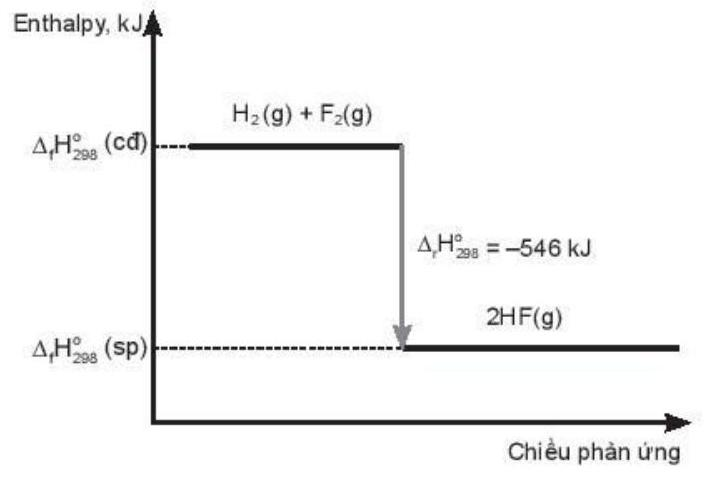
\includegraphics[max width=\textwidth, center]{2025_10_23_57761e23b8c46a11c3efg-45}

OT5.6. Biến thiên enthalpy của 2 phản ứng:

$$
\begin{array}{ll}
\mathrm{H}_{2}(g)+\frac{1}{2} \mathrm{O}_{2}(g) \rightarrow \mathrm{H}_{2} \mathrm{O}(l) & \Delta_{\mathrm{r}} \mathrm{H}_{298}^{\circ}=-285,84 \mathrm{~kJ} \\
\mathrm{HI}(g) \rightarrow \frac{1}{2} \mathrm{H}_{2}(g)+\frac{1}{2} \mathrm{l}_{2}(g) & \Delta_{\mathrm{r}} \mathrm{H}_{298}^{\circ}=-25,9 \mathrm{~kJ}
\end{array}
$$

OT5.7. Quá trình (a), phản ứng tự diễn ra.\\
Quá trình (b), phản ứng không tự diễn ra. Giá trị $\Delta_{\mathrm{r}} \mathrm{H}_{298}^{\circ}>0$.\\
Quá trình (c), phản ứng không tự diễn ra. Giá trị $\Delta_{\mathrm{r}} \mathrm{H}_{298}^{\circ}>0$.\\
OT5.8. Phản ứng trên toả nhiệt. Dùng tàn đóm đỏ để chứng minh khí sinh ra là oxygen. Ứng dụng của thí nghiệm trên trong thực tiễn\\
Hydrogenperoxide khử trùng, sát khuẩn nước, xử lí nước trong hồ. $\mathrm{H}_{2} \mathrm{O}_{2}$ nồng độ thấp hơn $3 \%$, được dùng để sát trùng vết thương, loại bỏ các mô chết. Sử dụng trong nuôi trồng thuỷ sinh.\\
OT5.9. a) Sơ đồ biểu diễn biến thiên enthalpy của phản ứng có dạng sau:\\
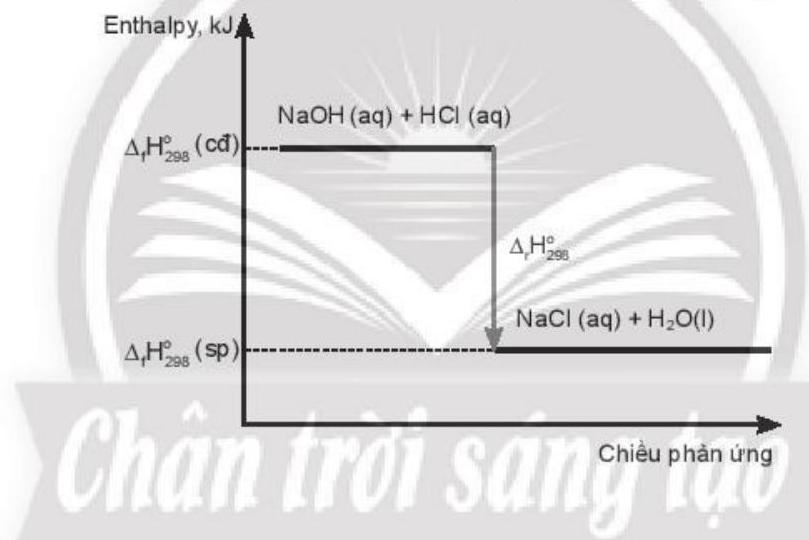
\includegraphics[max width=\textwidth, center]{2025_10_23_57761e23b8c46a11c3efg-46}\\
b) Lượng nhiệt toả ra khi dùng dung dịch có chứa 8 g NaOH trung hoà với lượng vừa đủ dung dịch HCl là:

$$
\mathrm{n}_{\mathrm{NaOH}}=0,2 \mathrm{~mol} \Rightarrow \Delta_{\mathrm{r}} \mathrm{H}_{298}^{\circ}=-57,3 \times 0,2=-114,6 \mathrm{~kJ}
$$

OT5.10. a) Phương trình hoá học:

$$
\begin{aligned}
& \mathrm{C}_{3} \mathrm{H}_{5}(\mathrm{OH})_{3}(a q)+3 \mathrm{HNO}_{3}(a q) \xrightarrow[\mathrm{t}^{0}]{\mathrm{xt}} \mathrm{C}_{3} \mathrm{H}_{5}\left(\mathrm{ONO}_{2}\right)_{3}(s)+3 \mathrm{H}_{2} \mathrm{O}(l) \\
& 4 \mathrm{C}_{3} \mathrm{H}_{5}\left(\mathrm{ONO}_{2}\right)_{3}(s) \xrightarrow{\mathrm{t}^{0}} 12 \mathrm{CO}_{2}(g)+10 \mathrm{H}_{2} \mathrm{O}(g)+\mathrm{O}_{2}(g)+6 \mathrm{~N}_{2}(g)
\end{aligned}
$$

b) $\mathrm{n}_{\mathrm{C}_{3} \mathrm{H}_{5}\left(\mathrm{ONO}_{2}\right)_{3}}=\frac{45,4}{227}=0,2(\mathrm{~mol})$

$$
4 \mathrm{C}_{3} \mathrm{H}_{5}\left(\mathrm{ONO}_{2}\right)_{3}(\mathrm{~s}) \xrightarrow{\mathrm{t}^{\circ}} 12 \mathrm{CO}_{2}(\mathrm{~g})+10 \mathrm{H}_{2} \mathrm{O}(\mathrm{~g})+\mathrm{O}_{2}(\mathrm{~g})+6 \mathrm{~N}_{2}(\mathrm{~g})
$$

$\begin{array}{lllll}\text { (mol) } 0,2 & 0,6 & 0,5 & 0,05 & 0,3\end{array}$\\
$\Rightarrow \sum \mathrm{n}_{\text {khihoi }}=0,6+0,5+0,05+0,3=1,45(\mathrm{~mol})$\\
c) Phân huỷ 1 mol (hay 227 g$) \mathrm{C}_{3} \mathrm{H}_{5}\left(\mathrm{ONO}_{2}\right)_{3} \rightarrow 1448 \mathrm{~kJ}$\\
$\Rightarrow$ Phân huỷ 1 kg hay $1000 \mathrm{~g} \mathrm{C}_{3} \mathrm{H}_{5}\left(\mathrm{ONO}_{2}\right)_{3} \rightarrow \frac{1000}{227} \times 1448=6378,85(\mathrm{~kJ})$\\
OT5.11. Ở điều kiện chuẩn, đốt cháy hoàn toàn $12 \mathrm{~g} \mathrm{H}_{2}$ lượng nhiệt toả ra $\Delta_{\mathrm{r}} \mathrm{H}_{298}^{\circ}=-171,504 \mathrm{~kJ}$. Cho $3,2 \mathrm{~g} \mathrm{~S}$ phản ứng hoàn toàn với oxygene để tạo ra $\mathrm{SO}_{3}(\mathrm{~g})$ cần cung cấp lượng nhiệt là $39,61 \mathrm{~kJ}$.

OT5.12. Silver bromide $(\mathrm{AgBr})$ là chất nhạy cảm với ánh sáng dùng để tráng lên phim. Dưới tác dụng của ánh sáng, nó phân huỷ thành kim loại bạc (ở dạng bột màu đen) bám trên tấm phim và bromine (ở dạng hơi).\\
$2 \mathrm{AgBr}(s) \xrightarrow{\mathrm{t}^{\circ}, \text { as }} 2 \mathrm{Ag}(s)+\mathrm{Br}_{2}(g)$\\
Phản ứng xảy ra là phản ứng thu nhiệt.\\
Sau khi chụp ảnh, phim được rửa bằng dung dịch $\mathrm{Na}_{2} \mathrm{~S}_{2} \mathrm{O}_{3}$ (chất xử lí ảnh), hoà $\tan \mathrm{AgBr}$ còn lại, trên phim chỉ còn lại Ag bám trên đó tạo hình ảnh âm bản cho tấm phim.\\
$\mathrm{AgBr}(s)+2 \mathrm{Na}_{2} \mathrm{~S}_{2} \mathrm{O}_{3}(a q) \rightarrow \mathrm{Na}_{3}\left[\mathrm{Ag}\left(\mathrm{S}_{2} \mathrm{O}_{3}\right)_{2}\right](a q)+\mathrm{NaBr}(a q)$ (phức sodium bis(thiosulfato)argentate(I))

OT5.13. $\mathrm{C}_{6} \mathrm{H}_{12} \mathrm{O}_{6}(s)+6 \mathrm{O}_{2}(g) \rightarrow 6 \mathrm{CO}_{2}(g)+6 \mathrm{H}_{2} \mathrm{O}(f) \quad \Delta_{\mathrm{r}} \mathrm{H}_{298}^{\circ}=-2803,0 \mathrm{~kJ} / \mathrm{mol}$\\
Năng lượng tối đa khi một người bệnh được truyền 1 chai 500 mL dung dịch glucose $5 \%(D=1,1)$ là: $\frac{27,5}{180} \times 2803,0=428,23 \mathrm{~kJ}$\\
OT5.14.\\
a) Mục đích pha trộn thêm chất tạo mùi đặc trưng vào khí gas để giúp phát hiện khí gas khi xảy ra sự cố rò rỉ.\\
b) Nhiệt dung riêng của nước: $1 \mathrm{kcal}=4,184 \mathrm{~kJ}$ (nhiệt lượng cần thiết tăng 1 lít nước lên $1^{\circ} \mathrm{C}$ ). Nhiệt lượng toả ra khi đốt cháy hoàn toàn 1 bình gas 12 kg :\\
Số mol propane $=\frac{3,6 \times 10^{3}}{44}=81,8181 \mathrm{~mol} \Rightarrow \Delta_{\mathrm{r}} \mathrm{H}_{298}^{\circ}=181636,36 \mathrm{~kJ}$\\
Số mol butane $=\frac{8,4 \times 10^{3}}{58}=144,8275 \mathrm{~mol} \Rightarrow \Delta_{\mathrm{r}} \mathrm{H}_{298}^{\circ}=416234,48 \mathrm{~kJ}$\\
Tồng năng lượng thu được: $597870,595 \mathrm{~kJ}$ với số ngày khoảng 60 ngày.

\section*{Chương 6. TỐC ĐỘ PHẢN ÚNG HOÁ HOC}
\section*{BÀI 15. PHƯƠNG TRİNH TỐC ĐỘ PHẢN ỨNG VÀ HẦNG SỐ TỐC ĐỘ PHẢN ỨNG}
15.1. Đáp án B.\\
15.2. Đáp án $A$.\\
15.3. Đáp án $C$.\\
15.4. Đáp án C.\\
15.5. Đáp án D.\\
15.6. Đáp án $C$.\\
15.7. Biểu thức tốc độ của phản ứng $\mathrm{CO}(g)+\mathrm{H}_{2} \mathrm{O}(g) \rightarrow \mathrm{CO}_{2}(g)+\mathrm{H}_{2}(g)$ là: $v=k \times \mathrm{C}_{\mathrm{CO}} \times \mathrm{C}_{\mathrm{H}_{2} \mathrm{O}}$. Khi nồng độ CO tăng 2 lần, ta có $v^{\prime}=k \times 2 \mathrm{C}_{\mathrm{CO}} \times \mathrm{C}_{\mathrm{H}_{2} \mathrm{O}}=2 v$, tốc độ phản ứng tăng 2 lần.\\
15.8. $\mathrm{Mg}(s)+2 \mathrm{HCl}(a q) \rightarrow \mathrm{MgCl}_{2}(a q)+\mathrm{H}_{2}(g)$

$$
0,2 \quad 0,1 \quad(\mathrm{M})
$$

Theo phương trình hoá học, vì bỏ qua sự thay đồi thể tích dung dịch sau phản ứng:\\
$\mathrm{C}_{\mathrm{M}}\left(\mathrm{MgCl}_{2}\right)=\frac{1}{2} \mathrm{C}_{\mathrm{M}}(\mathrm{HCl})=0,1(\mathrm{M})$.\\
Tốc độ trung bình của phản ứng tính theo $\mathrm{MgCl}_{2}$ trong 40 giây là:\\
$\bar{v}=\frac{0,1}{40}=2,5 \times 10^{-3}(\mathrm{M} / \mathrm{s})$\\
Vậy, tốc độ trung bình của phản ứng tính theo HCl và $\mathrm{MgCl}_{2}$ là bằng nhau.\\
15.9. a) Tốc độ trung bình của phản ứng

\begin{center}
\begin{tabular}{|c|c|c|c|}
\hline
\begin{tabular}{c}
Phản \\
úng \\
\end{tabular} & \begin{tabular}{c}
Lượng chất phản ứng \\
(mol) \\
\end{tabular} & \begin{tabular}{c}
Thời gian \\
(s) \\
\end{tabular} & \begin{tabular}{c}
Tốc độ phản úng \\
(mol/s) \\
\end{tabular} \\
\hline
1 & 2 & 30 & 0,067 \\
\hline
2 & 5 & 120 & 0,042 \\
\hline
3 & 1 & 90 & 0,011 \\
\hline
4 & 3,2 & 90 & 0,036 \\
\hline
5 & 5,9 & 30 & 0,197 \\
\hline
\end{tabular}
\end{center}

b) Phản ứng 5 xảy ra nhanh nhất và phản ứng 3 chậm nhất.\\
15.10. a) Tính tốc độ trung bình (mol/s) của phản ứng (1) là: $\bar{v}=\frac{2}{95 \times 60}=3,5 \times 10^{-4}(\mathrm{~mol} / \mathrm{s})$\\
b) Tốc độ trung bình của phản ứng (2) tương đương (1), khối lượng NaCl là:

$$
\mathrm{m}=\frac{2 \times 58,5}{95}=1,23(\mathrm{~g})
$$

15.11. Công thức tính tốc độ phản ứng: $\bar{v}=\frac{\Delta C}{\Delta t}$

Tốc độ phản ứng sau $4 \mathrm{~s}: \bar{v}=\frac{0,22-0,10}{4}=0,03(\mathrm{M} / \mathrm{s})$\\
15.12. Biểu thức tốc độ phản ứng: $\mathrm{V}=\mathrm{k} \times \mathrm{C}_{\mathrm{A}} \times \mathrm{C}_{\mathrm{B}}$.

Theo kết quả thực nghiệm 1: $k=\frac{V}{C_{A} \times C_{B}}=\frac{0,24}{0,2 \times 0,05}=24\left(\mathrm{M}^{-1} \cdot \mathrm{~s}^{-1}\right)$\\
Từ thực nghiệm 2 , tính được nồng độ chất A , từ thực nghiệm 3 , tính được nồng độ chất B :

$$
\mathrm{C}_{\mathrm{A}}=\frac{v}{k \times \mathrm{C}_{\mathrm{B}}}=\frac{0,20}{24 \times 0,03}=0,28(\mathrm{M}) ; \mathrm{C}_{\mathrm{B}}=\frac{v}{k \times \mathrm{C}_{\mathrm{A}}}=\frac{0,80}{24 \times 0,40}=0,28(\mathrm{M}) ;
$$

15.13. Phản ứng phân huỷ khí $\mathrm{N}_{2} \mathrm{O}_{5}$ xảy ra như sau: $2 \mathrm{~N}_{2} \mathrm{O}_{5}(g) \rightarrow 4 \mathrm{NO}_{2}(g)+\mathrm{O}_{2}(g)$\\
a) Biểu thức tính tốc độ trung bình của phản ứng là:

$$
\bar{v}=\frac{\Delta \mathrm{C}_{\mathrm{O}_{2}}}{\Delta \mathrm{t}}=\frac{1}{4} \times \frac{\Delta \mathrm{C}_{\mathrm{NO}_{2}}}{\Delta \mathrm{t}}=-\frac{1}{2} \times \frac{\Delta \mathrm{C}_{\mathrm{N}_{2} \mathrm{O}_{5}}}{\Delta \mathrm{t}}
$$

b) Theo hệ số cân bằng của phương trình, ta có

\begin{itemize}
  \item tốc độ tạo thành $\mathrm{NO}_{2}=4$ lần tốc độ tạo thành $\mathrm{O}_{2}=9,0 \times 10^{-6} \times 4=3,6 \times 10^{-5}(\mathrm{M} / \mathrm{s})$.
  \item tốc độ phân huỷ $\mathrm{N}_{2} \mathrm{O}_{5}=2$ lần tốc độ tạo thành $\mathrm{O}_{2}=9,0 \times 10^{-6} \times 2=1,8 \times 10^{-5}(\mathrm{M} / \mathrm{s})$.\\
15.14. Phương trình hoá học của phản ứng: $\quad 2 \mathrm{SO}_{2}(g)+\mathrm{O}_{2}(g) \rightarrow 2 \mathrm{SO}_{3}(g)$
\end{itemize}

Tốc độ trung bình của phản ứng được tính trong khoảng thời gian $\mathrm{t}_{1}=300(\mathrm{~s})$ đến $\mathrm{t}_{2}=720(\mathrm{~s}) \Rightarrow \Delta \mathrm{t}=720-300=420(\mathrm{~s}) ; \Delta \mathrm{C}=\mathrm{C}_{\text {sau }}-\mathrm{C}_{\text {đàu }}$.\\
Tốc độ trung bình của phản ứng: $\bar{v}=-\frac{1}{2} \times \frac{\Delta \mathrm{C}_{\mathrm{SO}_{2}}}{\Delta \mathrm{t}}=-\frac{\Delta \mathrm{C}_{\mathrm{O}_{2}}}{\Delta \mathrm{t}}=\frac{1}{2} \times \frac{\Delta \mathrm{C}_{\mathrm{SO}_{3}}}{\Delta \mathrm{t}}$\\
$\Rightarrow \bar{v}=\frac{1}{2} \times \frac{0,0270-0,0194}{420}=\frac{0,0500-0,0462}{420}=\frac{1}{2} \times \frac{0,0148-0,0072}{420}=9 \times 10^{-6}(\mathrm{M} / \mathrm{s})$

\section*{BÀI 16. CÁC YẾU TỐ ẢNH HƯỞNG ĐẾN TỐC ĐỘ PHẢN ỨNG}
16.1. Đáp án A .\\
16.2. Đáp án B.\\
16.3. Đáp án $A$.\\
16.4. Đáp án D.\\
16.5. Đáp án C.\\
16.6. Đáp án B.\\
16.7.

\begin{center}
\begin{tabular}{|l|l|}
\hline
Yếu tố ảnh hưởng & Tốc độ phản ứng \\
\hline
Đun nóng chất tham gia & Tăng \\
\hline
Thêm xúc tác phù hợp & Tăng \\
\hline
Pha loãng dung dịch & Giảm \\
\hline
Ngưng dùng enzyme (chất xúc tác) & Giảm \\
\hline
Giảm nhiệt độ & Giảm \\
\hline
Tăng nhiệt độ & Tăng \\
\hline
Giảm diện tích bề mặt & Giảm \\
\hline
Tăng nồng độ chất phản ứng & Tăng \\
\hline
Chia nhỏ chất phản ứng thành mảnh nhỏ & Tăng \\
\hline
\end{tabular}
\end{center}

16.8. Tăng nồng độ: Khi tăng nồng độ các chất tham gia phản ứng, sẽ tạo ra nhiều va chạm hiệu quả, tốc độ phản ứng tăng.\\
Tăng nhiệt độ: Khi đun nóng, năng lượng mà các phân tử thu được sẽ chuyển hoá thành động năng, chuyển động với tốc độ nhanh hơn, làm gia tăng tần số va chạm hiệu quả giữa các hạt, tốc độ phản ứng tăng.\\
Thêm chất xúc tác: Chất xúc tác làm giảm năng lượng hoạt hoá của chất tham gia phản ứng, phản ứng dễ xảy ra hơn hoặc tăng tốc độ phản ứng.\\
16.9.

\begin{center}
\begin{tabular}{|l|l|}
\hline
Tình huống & Yếu tố ảnh hưởng \\
\hline
Duy trì thổi không khí vào bếp để than cháy đều & Nồng độ \\
\hline
Than đá được nghiền nhỏ dùng trong quá trình luyện kim loại & Bề mặt tiếp xúc \\
\hline
Thức ăn được tiêu hoá trong dạ dày nhờ acid và enzyme & Xúc tác \\
\hline
Xác của một số loài động vật được bảo quản nguyên vẹn ở Bắc cực và Nam cực hàng ngàn năm & Nhiệt độ \\
\hline
Vụ nổ bụi xảy ra tại một xưởng cưa & Bề mặt tiếp xúc, nồng độ \\
\hline
\end{tabular}
\end{center}

16.10. Khối lượng chất rắn trước và sau phản ứng không thay đổi, chứng tỏ chất xúc tác không phải là chất phản ứng. Trong một số phản ứng, chất xúc tác tham gia phản ứng tạo thành hợp chất trung gian kém bền, sau đó tạo ra sản phẩm và chất xúc tác được bảo toàn về chất và lượng.\\
16.11. a) Ảnh hưởng bởi yếu tố nồng độ. Than cháy luôn cần oxygen để duy trì sự cháy, khi thổi không khí vào, làm tăng nồng độ oxygen, than cháy mạnh hơn.\\
b) Ảnh hưởng bởi yếu tố xúc tác. Xúc tác giúp phản ứng dễ xảy ra hơn.\\
c) Ảnh hưởng bởi yếu tố bề mặt tiếp xúc. Aluminum dạng bột có bề mặt tiếp xúc lớn hơn dạng lá, phản ứng xảy ra nhanh hơn.\\
d) Ảnh hưởng bởi yếu tố nhiệt độ. Quá trình bảo quản thực phẩm là hạn chế vi khuẩn hoạt động phá huỷ thức ăn, khi bảo quản trong tủ lạnh, nhiệt độ thấp sẽ giảm khả năng hoạt động của vi khuẩn, làm chậm quá trình phá huỷ thức ăn.\\
e) Ảnh hưởng bởi yếu tố nhiệt độ. Khi tăng áp suất, nhiệt độ sôi của nước tăng, thực phẩm nhanh chín hơn.\\
g) Ảnh hưởng bởi yếu tố chất xúc tác làm tăng tốc độ quá trình lên men.\\
16.12. Chè xanh nói riêng, thực phẩm nói chung, luôn chứa những thành phần có lợi cho sức khoẻ con người. Theo cơ địa mỗi người mà thu nạp vào cơ thể lượng thực phẩm phù hợp, cân đối, như người thừa cân dùng thực phẩm ît chất béo, tăng cường chất xơ, kết hợp tập thể dục; người bị Gout hạn chế dùng thực phẩm chứa chất đạm, ... Lá chè xanh chứa nhiều thành phần có tác dụng ngăn ngừa bệnh tật, nhưng ở hàm lượng (yếu tố nồng độ) cao, gây ra những triệu chứng khó chịu, suy giảm sức khoẻ, bệnh tật.\\
16.13. Thiết bị sử dụng các kim loại quý như $\mathrm{Pt}, \mathrm{Rh}, \mathrm{Pd}$ để thúc đẩy quá trình nhường và nhận electron của các chất có trong khí thải thành những chất ít ô nhiễm môi trường:\\
Quá trình oxi hoá các hydrocarbon $\left(\mathrm{C}_{\mathrm{x}} \mathrm{H}_{\mathrm{y}}\right)$, carbon monoxide:\\
$4 \mathrm{C}_{\mathrm{x}} \mathrm{H}_{\mathrm{y}}(g)+(4 \mathrm{x}+\mathrm{y}) \mathrm{O}_{2}(g) \rightarrow 4 \mathrm{xCO}_{2}(g)+2 \mathrm{yH}_{2} \mathrm{O}(g)$\\
$2 \mathrm{CO}(g)+\mathrm{O}_{2}(g) \rightarrow 2 \mathrm{CO}_{2}(g)$\\
Quá trình khử các oxide của nitrogen:\\
$2 \mathrm{Na}_{\mathrm{a}} \mathrm{O}(g) \rightarrow \mathrm{aN}_{2}(g)+\mathrm{bO}_{2}(g)$\\
Chỉ có chất khí trong khi thải tham gia phản ứng, các kim loại $\mathrm{Pt}, \mathrm{Rh}, \mathrm{Pd}$ đóng vai trò chất xúc tác. Yếu tố xúc tác được vận dụng trong thiết bị trên.\\
16.14. Bột mì trên dĩa hay tập trung một chỗ thì rất khó cháy, nếu được phun tơi dạng bụi sẽ dễ cháy hơn, là do bề mặt tiếp xúc tăng lên rất nhiều. Khi đủ 5 tác nhân: nguồn oxygen, nguồn nhiệt, bụi có thể cháy được, nồng độ bụi để đạt được vụ nổ và không gian đủ kín sẽ gây ra nổ thứ cấp (nổ dây chuyền).\\
Để ngăn ngừa và hạn chế nổ bụi, có thể can thiệp vào 2 yếu tố chính: giảm nồng độ hạt bụi và kiểm soát nguồn nhiệt trong khu vực sản xuất (hệ thống điện, nguồn điện, ổ cắm, ...).\\
16.15. Ý (1) vận dụng yếu tố bề mặt tiếp xúc; ý (2) là yếu tố nồng độ, tỉ lệ nhiên liệu - không khí phù hợp đảm bảo các phản ứng xảy ra hoàn toàn; ý (3) là nồng độ, khi tăng/giảm vận tốc, hệ thống sẽ tăng/giảm tỉ lệ nhiên liệu - không khí tương ứng.\\
16.16. a) Tốc độ phản ứng của phản ứng thuỷ phân aspirin theo thời gian

\begin{center}
\begin{tabular}{|l|l|l|l|}
\hline
Thời gian (h) & Nồng độ aspirin (M) & Nồng độ salicylic acid (M) & Tốc độ phản ứng (M/h) \\
\hline
0 & $5,55 \times 10^{-3}$ & 0 & 0 \\
\hline
2 & $5,51 \times 10^{-3}$ & $0,040 \times 10^{-3}$ & $2,000 \times 10^{-5}$ \\
\hline
5 & $5,45 \times 10^{-3}$ & $0,10 \times 10^{-3}$ & $2,000 \times 10^{-5}$ \\
\hline
10 & $5,35 \times 10^{-3}$ & $0,20 \times 10^{-3}$ & $2,000 \times 10^{-5}$ \\
\hline
20 & $5,15 \times 10^{-3}$ & $0,40 \times 10^{-3}$ & $2,000 \times 10^{-5}$ \\
\hline
30 & $4,96 \times 10^{-3}$ & $0,59 \times 10^{-3}$ & $1,967 \times 10^{-5}$ \\
\hline
40 & $4,78 \times 10^{-3}$ & $0,77 \times 10^{-3}$ & $1,925 \times 10^{-5}$ \\
\hline
50 & $4,61 \times 10^{-3}$ & $0,94 \times 10^{-3}$ & $1,880 \times 10^{-5}$ \\
\hline
100 & $3,83 \times 10^{-3}$ & $1,72 \times 10^{-3}$ & $1,720 \times 10^{-5}$ \\
\hline
200 & $2,64 \times 10^{-3}$ & $2,91 \times 10^{-3}$ & $1,455 \times 10^{-5}$ \\
\hline
300 & $1,82 \times 10^{-3}$ & $3,73 \times 10^{-3}$ & $1,243 \times 10^{-5}$ \\
\hline
\end{tabular}
\end{center}

b) Trong khoảng thời gian 20 giờ đầu tiên của phản ứng thuỷ phân, nồng độ aspirin đủ lớn để tạo ra số va chạm hiệu quả tương đương nhau, tốc độ trung bình phản ứng đạt $2,000 \times 10^{-5}(\mathrm{M} / \mathrm{h})$, sau đó, tốc độ phản ứng thuỷ phân aspirin chậm dần. Khi nồng độ aspirin giảm, làm giảm tần số va chạm hiệu quả giữa các phân tử, tốc độ phản ứng giảm.\\
c) Đồ thị biểu diễn sự biến thiên nồng độ chất tham gia và sản phẩm theo thời gian.\\
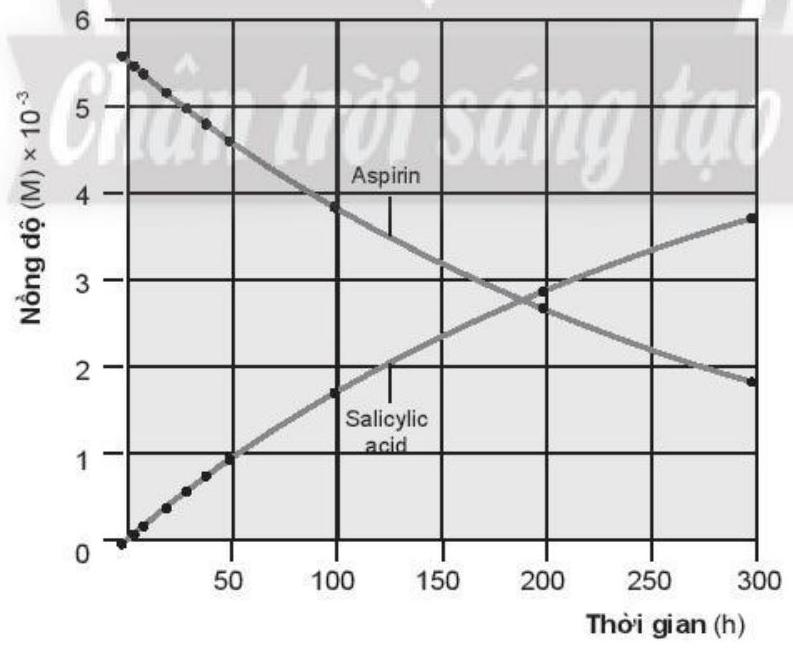
\includegraphics[max width=\textwidth, center]{2025_10_23_57761e23b8c46a11c3efg-53}\\
16.17. HS tiến hành thí nghiệm.

\section*{ÔN TẬP CHƯƠNG 6}
OT6.1. Đáp án B.\\
OT6.2. Đáp án A.\\
OT6.3. Đáp án D.\\
OT6.4. Thứ tự cho vào cốc trà nóng là đường, đá viên. Vì đường tan tốt hơn trong nước nóng.

OT6.5. Biểu thức tốc độ: $v=k \times \mathrm{C}_{\mathrm{CO}}^{2} \times \mathrm{C}_{\mathrm{O}_{2}}, k$ là hằng số tốc độ phản ứng.\\
Khi nồng độ $\mathrm{mol} / \mathrm{L}$ của CO và $\mathrm{O}_{2}$ là 1 M , thì: $v=k \times 1^{2} \times 1=k$\\
$k$ là tốc độ riêng của phản ứng $2 \mathrm{CO}(g)+\mathrm{O}_{2}(g) \rightarrow 2 \mathrm{CO}_{2}(g)$.\\
OT6.6. Tính tốc độ trung bình ( $\mathrm{mL} / \mathrm{s}$ ) của phản ứng trong 60 giây:

$$
\bar{v}=\frac{30}{60}=0,5(\mathrm{~mL} / \mathrm{s})
$$

OT6.7. a) Tốc độ trung bình của phản ứng trong phút thứ nhất:

$$
\bar{v}=\frac{0,1563-0,1496}{60}=1,12 \times 10^{-4}(\mathrm{M} / \mathrm{s})
$$

Tốc độ trung bình của phản ứng trong phút thứ 2 :

$$
\bar{v}=\frac{0,1496-0,1431}{60}=1,08 \times 10^{-4}(\mathrm{M} / \mathrm{s})
$$

b) Tốc độ trung bình của phản ứng trong 2 phút không bằng nhau, vì nồng độ chất A giảm theo thời gian, làm giảm số va chạm hiệu quả nên tốc độ phản ứng giảm.

OT6.8. Tốc độ trung bình của phản ứng được tính trong khoảng thời gian $\mathrm{t}_{1}=240(\mathrm{~s})$ đến $\mathrm{t}_{2}=600(\mathrm{~s}) \Rightarrow \Delta \mathrm{t}=600-240=360(\mathrm{~s}) ; \Delta \mathrm{C}=\mathrm{C}_{\text {sau }}-\mathrm{C}_{\text {đàu }}$.\\
Tốc độ trung bình của phản ứng: $\bar{v}=-\frac{1}{2} \times \frac{\Delta \mathrm{C}_{\mathrm{N}_{2} \mathrm{O}_{5}}}{\Delta \mathrm{t}}=\frac{1}{4} \times \frac{\Delta \mathrm{C}_{\mathrm{NO}_{2}}}{\Delta \mathrm{t}}=\frac{\Delta \mathrm{C}_{\mathrm{O}_{2}}}{\Delta \mathrm{t}}$\\
$\bar{v}=\frac{1}{2} \times \frac{0,0388-0,0196}{360}=\frac{1}{4} \times \frac{0,0699-0,0315}{360}=\frac{0,0175-0,0079}{360}=2,67 \times 10^{-5}(\mathrm{M} / \mathrm{s})$

OT6.9. a) Tốc độ phản ứng phân huỷ $\mathrm{H}_{2} \mathrm{O}_{2}$ theo thời gian

\begin{center}
\begin{tabular}{|l|l|l|}
\hline
Thời gian (s) & $\mathrm{H}_{2} \mathrm{O}_{2}(\mathrm{~mol} / \mathrm{L})$ & Tốc độ phản ứng (mol/L.s) \\
\hline
0 & 1,000 & 0 \\
\hline
120 & 0,910 & $7,5 \times 10^{-4}$ \\
\hline
300 & 0,780 & $7,3 \times 10^{-4}$ \\
\hline
600 & 0,590 & $6,8 \times 10^{-4}$ \\
\hline
1200 & 0,370 & $5,3 \times 10^{-4}$ \\
\hline
1800 & 0,220 & $4,3 \times 10^{-4}$ \\
\hline
2400 & 0,130 & $3,6 \times 10^{-4}$ \\
\hline
3000 & 0,082 & $3,1 \times 10^{-4}$ \\
\hline
3600 & 0,050 & $2,6 \times 10^{-4}$ \\
\hline
\end{tabular}
\end{center}

b) Tốc độ phản ứng giảm dần theo thời gian. Tốc độ phản ứng phụ thuộc vào nồng độ chất tham gia, theo thời gian, nồng độ $\mathrm{H}_{2} \mathrm{O}_{2}$ giảm dần nên tốc độ phản ứng giảm.

\section*{Chuong ᄀ. NGUYÊN TÓ NHÓM VIIA - HALOGEN}
\section*{BÀI 17. TÍNH CHÁT VẬT LÍ VÀ HOÁ HỌC CÁC ĐƠN CHẤT NHÓM VIIA}
17.1. Đáp án $C$.\\
17.2. Đáp án B.\\
17.3. Đáp án A .\\
17.4. Đáp án B.\\
17.5. Đáp án $C$.\\
17.6. Đáp án B.\\
17.7. Đáp án C.\\
17.8. Đáp án A .\\
17.9. Đáp án B.\\
17.10. Đáp án B.\\
17.11. Đáp án D .\\
17.12. Đáp án $B$.\\
17.13. Đáp án $A$.\\
17.14. Đáp án B.\\
17.15. Đáp án D .\\
17.16. Từ $F$ đến $I$, độ âm điện giảm dần, khả năng liên kết với nguyên tử hydrogen giảm dần.\\
Thứ tự giảm dần khả năng liên kết với hydrogen: $\mathrm{F}>\mathrm{Cl}>\mathrm{Br}>\mathrm{I}$.

\begin{center}
\begin{tabular}{|c|c|c|c|c|}
\hline
Hydrogen halide & $\mathbf{H F}$ & $\mathbf{H C I}$ & $\mathbf{H B r}$ & $\mathbf{H I}$ \\
\hline
\begin{tabular}{c}
Hiệu độ âm điên \\
trong phân tử HX \\
\end{tabular} & $3,98-2,20=1,78$ & $3,16-2,20=0,96$ & $2,96-2,20=0,74$ & $2,66-2,20=0,46$ \\
\hline
\end{tabular}
\end{center}

Độ phân cực của phân tử hydrogen halide: $\mathrm{HF}>\mathrm{HCl}>\mathrm{HBr}>\mathrm{HI}$.\\
17.17. $\mathrm{Cl}_{2}$ có tính oxi hoá mạnh hơn $\mathrm{Br}_{2}$, nên $\mathrm{Cl}_{2}$ oxi hoá ion $\mathrm{Br}^{-}$trong dung dịch muối thành $\mathrm{Br}_{2} . \mathrm{Br}_{2}$ có tính oxi hoá mạnh hơn $\mathrm{I}_{2}$, nên $\mathrm{Br}_{2}$ oxi hoá ion $\mathrm{I}^{-}$trong dung dịch muối thành $\mathrm{I}_{2}$.\\
Thứ tự giảm dần tính oxi hoá: $\mathrm{Cl}_{2}>\mathrm{Br}_{2}>\mathrm{I}_{2}$.\\
17.18. a) $\stackrel{0}{\mathrm{Br}_{2}}+2 \mathrm{~K} \rightarrow 2 \mathrm{KBr}\left(\mathrm{Br}_{2}\right.$ có vai trò là chất oxi hoá)\\
b) $2 \stackrel{\circ}{\mathrm{~F}}_{2}+2 \mathrm{H}_{2} \mathrm{O} \rightarrow 4 \mathrm{H}^{-1}+\mathrm{O}_{2}\left(\mathrm{~F}_{2}\right.$ là chất oxi hoá)\\
c) $2 \stackrel{0}{\mathrm{Cl}}{ }_{2}+2 \mathrm{Ca}(\mathrm{OH})_{2} \rightarrow \mathrm{CaCl}{ }_{2}^{-1}+\mathrm{Ca}(\stackrel{+1}{\mathrm{ClO}})_{2}+2 \mathrm{H}_{2} \mathrm{O}\left(\mathrm{Cl}_{2}\right.$ là chất oxi hoá và là chất khử)\\
d) $\stackrel{0}{\mathrm{Cl}}_{2}+2 \mathrm{NaI} \rightarrow 2 \mathrm{NaCl}+\mathrm{I}_{2}\left(\mathrm{Cl}_{2}\right.$ là chất oxi hoá)\\
17.19.

Bước 1: Hoà tan mẫu muối vào nước, thêm vài giọt hồ tinh bột, hỗn hợp dung dịch không màu.\\
Bước 2: Nhỏ vài giọt nước chlorine vào hỗn hợp dung dịch trên, xuất hiện màu xanh đen.

$$
\mathrm{Cl}_{2}+2 \mathrm{NaI} \rightarrow 2 \mathrm{NaCl}+\mathrm{I}_{2} \downarrow
$$

Đặc trưng của iodine gặp hồ tinh bột, dung dịch có màu xanh đen.\\
17.20.

Chlorine (CI) $\quad 1 s^{2} 2 s^{2} 2 p^{6} 3 s^{2} 3 p^{5}$\\
Bromine ( Br ) $\quad 1 \mathrm{~s}^{2} 2 \mathrm{~s}^{2} 2 \mathrm{p}^{6} 3 \mathrm{~s}^{2} 3 \mathrm{p}^{6} 3 \mathrm{~d}^{10} 4 \mathrm{~s}^{2} 4 \mathrm{p}^{5}$\\
lodine (I) $\quad 1 s^{2} 2 s^{2} 2 p^{6} 3 s^{2} 3 p^{6} 3 d^{10} 4 s^{2} 4 p^{6} 4 d^{10} 5 s^{2} 5 p^{5}$.\\
Cấu hình electron lớp ngoài cùng của nguyên tử halogen $n s^{2} n p^{5}$, có 1 electron không ghép đôi; chlorine, bromine, iodine tạo hợp chất có mức oxi hoá -1 khi liên kết với nguyên tử có độ âm điện nhỏ hơn như kim loại, hydrogen, ... và tạo mức oxi hoá +1 khi liên kết với nguyên tử có độ âm điện lớn hơn như oxygen, fluorine, ... Ngoài ra, chlorine, bromine, iodine còn các ô lượng tử chưa lấp đầy, có thể xảy ra các quá trình kích thích electron lên phân mức năng lượng cao hơn, tạo ra mức oxi hoá $+3,+5,+7$. Vì vậy, các số oxi hoá chẵn không đặc trưng đối với halogen trong hợp chất.\\
17.21. Cấu hình electron lớp ngoài cùng của nguyên tử halogen $n s^{2} n p^{5}$, có 1 electron không ghép đôi; chlorine, bromine, iodine tạo hợp chất có mức oxi hoá -1 khi liên kết với nguyên tử có độ âm điện nhỏ hơn như kim loại, hydrogen, ... và\\
tạo mức oxi hoá +1 khi liên kết với nguyên tử có độ âm điện lớn hơn như oxygen, fluorine, ... Ngoài ra, chlorine, bromine, iodine còn các ô lượng tử chưa lấp đầy, có thể xảy ra các quá trình kích thích electron lên phân mức năng lượng cao hơn, tạo ra mức oxi hoá $+3,+5,+7$.

\begin{figure}[h]
\begin{center}
  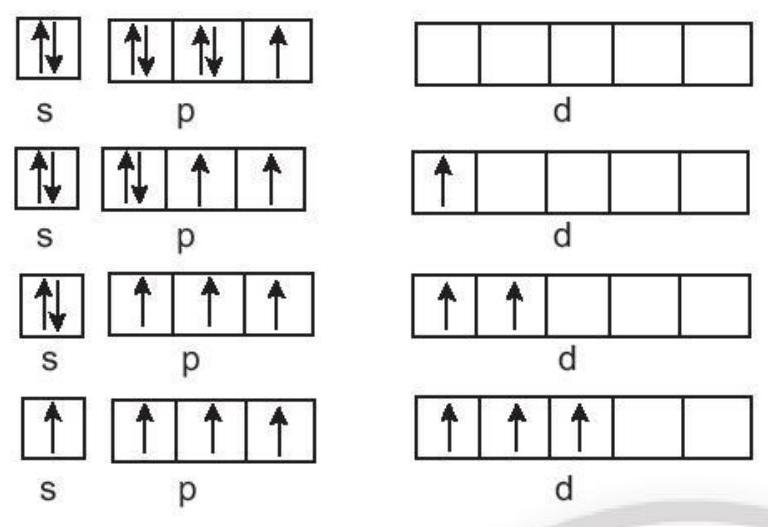
\includegraphics[width=\textwidth]{2025_10_23_57761e23b8c46a11c3efg-58}
\captionsetup{labelformat=empty}
\caption{Cấu hình electron của fluorine là \$1 s\^{}\{2} 2 s\^{}\{2\} 2 p\^{}\{5\}\$, ở lớp electron ngoài cùng có 1 electron không ghép đôi, không có ô lượng tử trống, khi hình thành liên kết hoá học, không có nguyên tử nào có độ âm điện lớn hơn fluorine đủ đề cung cấp năng lượng cho quá trình kích thích, vì vậy, fluorine chỉ thể hiện mức oxi hoá -1 trong các hợp chất.\}\end{center}
\end{figure}

17.22. Chất tan dễ dàng hoà tan trong dung môi có cùng bản chất: chất tan phân cực dễ tan trong dung môi phân cực và ngược lại. Đơn chất halogen là chất không phân cực nên dễ tan trong các dung môi không phân cực như hexane, carbon tetrachloride và ît tan trong dung môi phân cực như nước)\\
17.23. Dựa trên kết quả thực nghiệm về độ hoà tan của các halogen trong nước ở $25^{\circ} \mathrm{C}$, fluorine phản ưng mãnh liệt với nước theo phương trình: $2 \mathrm{~F}_{2}+2 \mathrm{H}_{2} \mathrm{O} \rightarrow 4 \mathrm{HF}+\mathrm{O}_{2}$, nên không tồn tại nước fluorine. Các halogen còn lại tác dụng chậm và tan một phần trong nước tạo thành nước halogen tương ứng.\\
17.24. Phương trình hoá học của phản ứng:

$$
\mathrm{Cl}_{2}+2 \mathrm{NaBr} \rightarrow 2 \mathrm{NaCl}+\mathrm{Br}_{2}
$$

Bước 1: NaBr là hợp chất ion, phân tử phân cực mạnh nên tan tốt trong nước, dung dịch đồng nhất, không màu\\
Bước 2: Hexane là chất hữu cơ không phân cực, hổn hợp dung dịch muối NaBr và hexane không tan vào nhau, hexane nhẹ hơn nên phân lớp phía trên.\\
Bước 3: $\mathrm{Br}_{2}$ được tạo ra dễ tan trong hexane, lớp chất lỏng phía trên có màu da cam.\\
Thí nghiệm chứng minh tính tan của đơn chất halogen trong 2 loại dung môi và chứng minh tính oxi hoá của $\mathrm{Cl}_{2}$ mạnh hơn $\mathrm{Br}_{2}$.\\
17.25.

\begin{center}
\begin{tabular}{|l|l|l|l|}
\hline
\multirow{2}{*}{STT} & \multirow{2}{*}{Phát biểu} & \multicolumn{2}{|r|}{Xác nhận} \\
\hline
 &  & Đúng & Sai \\
\hline
1 & Halogen vừa có tính oxi hoá, vừa có tính khử &  & $\times$ \\
\hline
2 & Nước chlorine và Javel đều có tính tẩy màu & $\times$ &  \\
\hline
3 & Halogen tồn tại cả đơn chất và hợp chất trong tự nhiên &  & $\times$ \\
\hline
4 & $\mathrm{Cl}_{2}$ có tính oxi hoá mạnh hơn $\mathrm{Br}_{2}$ & $\times$ &  \\
\hline
5 & $\mathrm{Cl}_{2}$ khử được $\mathrm{I}^{-}$trong dung dịch NaI thành $\mathrm{I}_{2}$ &  & $\times$ \\
\hline
6 & Nhỏ nước iodine vào mặt cắt củ khoai, xuất hiện màu xanh đen & $\times$ &  \\
\hline
7 & Hợp chất của fluorine làm thuốc chống sâu răng, chất dẻo Teflon & $\times$ &  \\
\hline
\end{tabular}
\end{center}

17.26. $1 \mathrm{~m}^{3}=1000$ lít

Để xử lí 1 lít nước cần 11 mg chlorine, nhà máy xử lị $3000 \mathrm{~m}^{3}$ nước/ ngày cần khối lượng chlorine là: $3000 \times 11 \times 1000=33 \times 10^{6} \mathrm{mg}=33 \mathrm{~kg}$.\\
17.27. Phương trình hoá học của phản ứng:\\
$\mathrm{Cl}_{2}+2 \mathrm{KI} \rightarrow 2 \mathrm{KCl}+\mathrm{I}_{2}$,\\
$\mathrm{I}_{2}+2 \mathrm{Na}_{2} \mathrm{~S}_{2} \mathrm{O}_{3} \rightarrow 2 \mathrm{NaI}+\mathrm{Na}_{2} \mathrm{~S}_{4} \mathrm{O}_{6}$.\\
Tính theo đơn vị mL và mg .\\
Số mol $\mathrm{Na}_{2} \mathrm{~S}_{2} \mathrm{O}_{3}$ phản ứng: $\mathrm{n}=0,01 \times 0,28=2,8 \times 10^{-3}(\mathrm{~mol})$\\
Theo tỉ lệ các chất trong phương trình, số mol $\mathrm{Cl}_{2}$ bằng $1 / 2$ số mol $\mathrm{Na}_{2} \mathrm{~S}_{2} \mathrm{O}_{3}$ :\\
$\mathrm{n}=1,4 \times 10^{-3}(\mathrm{~mol})$.\\
Khối lượng $\mathrm{Cl}_{2}$ có trong 100 ml dung dịch mẫu cần kiểm tra:\\
$\mathrm{m}=1,4 \times 10^{-3} \times 71=0,0994(\mathrm{mg})$\\
Trong 1 L dung dịch mẫu, khối lượng $\mathrm{Cl}_{2}$ là: $0,0994 \times 10=0,994(\mathrm{mg})$.\\
So sánh với tiêu chuẩn chất lượng sản phẩm về dư lượng chlorine không vượt quá $1 \mathrm{mg} / \mathrm{L}$, mẫu sản phẩm trên đủ tiêu chuẩn xuất khẩu.

\section*{BÀI 18. HYDROGEN HALIDE VÀ MỘT SỐ PHẢN ỨNG CỦA ION HALIDE}
18.1. Đáp án D.\\
18.2. Đáp án B.\\
18.3. Đáp án C.\\
18.4. Đáp án D.\\
18.5. Đáp án D.\\
18.6. Đáp án B.\\
18.7. Đáp án A .\\
18.8. Đáp án D.\\
18.9. Đáp án B.\\
18.10. Đáp án $A$.\\
18.11. Đáp án $B$.\\
18.12. Đáp án $A$.\\
18.13. Đáp án $C$.\\
18.14. Hydrogen chloride được điều chế bằng cách cho tinh thể sodium chloride tác dụng với sulfuric acid đặc, được gọi là phương pháp sulfate hoá. Phương pháp sulfate hoá điều chế được HF và HCl , vì ion $\mathrm{F}^{-}, \mathrm{Cl}^{-}$có tính khử không đủ mạnh để khử dung dịch $\mathrm{H}_{2} \mathrm{SO}_{4}$ đặc. Ion $\mathrm{Br}^{-}, \mathrm{I}^{-}$có tính khử mạnh hơn $\mathrm{F}^{-}$, $\mathrm{Cl}^{-}$nên khử được $\mathrm{H}_{2} \mathrm{SO}_{4}$ đặc, tạo ra $\mathrm{Br}_{2}$ và $\mathrm{I}_{2}$, không thu được $\mathrm{HBr}, \mathrm{HI}$. Để điều chế HBr và HI , có thể thay thế $\mathrm{H}_{2} \mathrm{SO}_{4}$ bằng acid $\mathrm{H}_{3} \mathrm{PO}_{4}$ đặc:

$$
\begin{aligned}
& 2 \mathrm{NaBr}(s)+\mathrm{H}_{3} \mathrm{PO}_{4}(l) \rightarrow \mathrm{Na}_{2} \mathrm{HPO}_{4}(s)+2 \mathrm{HBr}(g) \\
& 2 \mathrm{NaI}(s)+\mathrm{H}_{3} \mathrm{PO}_{4}(l) \rightarrow \mathrm{Na}_{2} \mathrm{HPO}_{4}(s)+2 \mathrm{HI}(g)
\end{aligned}
$$

Hoặc đun nóng hỗn hợp khí $\mathrm{H}_{2}$ và hơi $\mathrm{Br}_{2}: \mathrm{H}_{2}(g)+\mathrm{Br}_{2}(g) \rightarrow 2 \mathrm{HBr}(g)$\\
18.15. HBr và HI đều là chất khử mạnh, sau một thời gian sử dụng, ảnh hưởng của không khí, oxygen trong không khí oxi hoá 2 ion $\mathrm{Br}^{-}$và $\mathrm{I}^{-}$thành halogen tương ứng là $\mathrm{Br}_{2}$ có màu vàng, $\mathrm{I}_{2}$ trong dung dịch $\mathrm{I}^{-}$có màu vàng đậm, dung dịch sẩm màu nhanh hơn.

$$
\begin{aligned}
& 4 \mathrm{HBr}(a q)+\mathrm{O}_{2}(g) \rightarrow 2 \mathrm{H}_{2} \mathrm{O}(l)+2 \mathrm{Br}_{2}(a q) \\
& 4 \mathrm{HI}(a q)+\mathrm{O}_{2}(g) \rightarrow 2 \mathrm{H}_{2} \mathrm{O}(l)+2 \mathrm{I}_{2}(a q)
\end{aligned}
$$

18.16.\\
a) Theo chiều từ HF đến HI , giá trị $\mathrm{K}_{\mathrm{a}}$ tăng dần nên tính acid tăng dần. Vậy, tính acid giảm dần theo thứ tự: $\mathrm{HI}>\mathrm{HCl}>\mathrm{HBr}>\mathrm{HF}$.\\
b) Năng lượng liên kết càng lớn, độ dài liên kết $\mathrm{H}-\mathrm{X}$ càng ngắn, liên kết càng bền, trong dung dịch, tính acid càng yếu. Từ HF đến HI , năng lượng liên kết giảm, độ dài liên kết sẽ tăng, nên trong dung dịch, tính acid cũng tăng dần.\\
18.17. Phương trình hoá học của phản ứng:

$$
\mathrm{Mg}(s)+2 \mathrm{HCl}(a q) \rightarrow \mathrm{MgCl}_{2}(a q)+\mathrm{H}_{2}(g)
$$

Đặt x là số mol của Mg cho vào dung dịch $\mathrm{HCl} \Rightarrow \mathrm{n}_{\mathrm{H}_{2}}=\mathrm{x}$\\
Áp dụng định luật bảo toàn khối lượng: $\mathrm{m}_{\mathrm{Mg}}+\mathrm{m}_{\text {dung dich HCI }}=\mathrm{m}_{\text {dung dich sau phàn ưng }}+\mathrm{m}_{\mathrm{H}_{2}} \Rightarrow 24 \mathrm{x}+100=105,5+2 \mathrm{x} \Rightarrow \mathrm{x}=0,25(\mathrm{~mol})$\\
a) $\mathrm{m}_{\mathrm{Mg}}=0,25 \times 24=6(\mathrm{~g})$\\
b) $\mathrm{m}_{\mathrm{MgCl}_{2}}=0,25 \times 95=23,75(\mathrm{~g})$\\
$\mathrm{V}_{\mathrm{H}_{2}}=0,25 \times 24,79=6,2(\mathrm{~L})$\\
18.18.

Nhóm trẻ sơ sinh, khối lượng NaCl cần thiết là $0,3 \mathrm{~g}$, khối lượng $\mathrm{Cl}^{-}$ tương ứng là:

$$
m=\frac{0,3}{58,5} \times 35,5=0,182(g)=182(m g)
$$

Nhóm trẻ dưới 1 tuổi, khối lượng NaCl cần thiết là $1,5 \mathrm{~g}$, khối lượng $\mathrm{Cl}^{-}$ tương ứng là:

$$
m=182 \times 5=910(\mathrm{mg})
$$

Nhóm trẻ dưới 2 tuổi, khối lượng NaCl cần thiết là $2,3 \mathrm{~g}$, khối lượng $\mathrm{Cl}^{-}$ tương ứng là:

$$
m=\frac{2,3 \times 182}{0,3}=1395(\mathrm{mg})
$$

18.19.

\begin{itemize}
  \item Trong 100 gram muối i-ốt có chứa hàm lượng iodide là $2200 \mu \mathrm{~g}$;
\end{itemize}

\begin{itemize}
  \item Hàm lượng iodide tối thiểu ở mức $66 \mu \mathrm{~g} /$ ngày, thì lượng muối i-ốt cần dùng là:
\end{itemize}

$$
\mathrm{m}=\frac{66 \times 100}{2200}=3(\mathrm{~g})
$$

\begin{itemize}
  \item Hàm lượng iodide tối đa ở mức $110 \mu \mathrm{~g} / n$ gày, thì lượng muối i-ốt cần dùng là:
\end{itemize}

$$
\mathrm{m}=\frac{110 \times 100}{2200}=5(\mathrm{~g})
$$

\begin{itemize}
  \item Vậy, đối với loại muối i-ốt có hàm lượng iodide là $2200 \mu \mathrm{~g} / 100$ gam muối, lượng muối cần dùng mỗi ngày từ $3-5$ gam.
\end{itemize}

\begin{itemize}
  \item Trong 100 gram muối i-ốt có chứa hàm lượng iodide là $2500 \mu \mathrm{~g}$;
\end{itemize}

\begin{itemize}
  \item Hàm lượng iodide tối thiểu ở mức $66 \mu \mathrm{~g} /$ ngày, thì lượng muối i-ốt cần dùng là:
\end{itemize}

$$
\mathrm{m}=\frac{66 \times 100}{2500}=2,64(\mathrm{~g})
$$

\begin{itemize}
  \item Hàm lượng iodide tối đa ở mức $110 \mu \mathrm{~g} / \mathrm{ng}$ ày, thì lượng muối i-ốt cần dùng là:
\end{itemize}

$$
\mathrm{m}=\frac{110 \times 100}{2500}=4,4(\mathrm{~g})
$$

\begin{itemize}
  \item Vậy, đối với loại muối i-ốt có hàm lượng iodide là $2500 \mu \mathrm{~g} / 100$ gam muối, lượng muối cần dùng mỗi ngày từ $2,64-4,4$ gam.\\
18.20. Có khoảng $1000 \mu \mathrm{~g}\left(10^{-3} \mathrm{~g}\right)$ iodide trong 100 gam tảo bẹ khô
\end{itemize}

Để sản xuất 1 tấn ion iodide $\left(I^{-}\right)$cần khối lượng tảo bẹ khô là:

$$
\mathrm{m}=\frac{1 \times 100}{10^{-3}}=10^{5} \text { tấn }=0,1 \text { triệu tấn. }
$$

18.21. a) Mỗi lít nước biển chứa khoảng 36 g muối. Để thu được 426500 tấn muối/ năm thì thể tích nước biển cần dẫn vào ruộng muối là:

$$
\frac{426500 \times 10^{6}}{36}=1,1847 \times 10^{10}(\mathrm{~L})=11,847 \times 10^{6}\left(\mathrm{~m}^{3}\right)
$$

Để đạt được 650000 tấn/năm vào năm 2030, thì thể tích nước biển cần là:

$$
\frac{650000 \times 10^{6}}{36}=1,8056 \times 10^{10}(\mathrm{~L})=18,056 \times 10^{6}\left(\mathrm{~m}^{3}\right)
$$

b) Hàm lượng ion $\mathrm{Cl}^{-}$chiếm khoảng $55,04 \%$, khối lượng $\mathrm{Cl}^{-}$được khai thác hàng năm là: $\mathrm{m}_{\mathrm{cl}}=426500 \times 55,04 \%=234745,6$ (tấn)\\
Với khối lượng 650000 tấn, khối lượng $\mathrm{Cl}^{-}$được khai thác là:

$$
\mathrm{m}_{\mathrm{cl}}=650000 \times 55,04 \%=357760 \text { (tấn). }
$$

Các phép tsoán bỏ qua sai số của cân phân tích, cân kĩ thuật, có các sai số từ $1-5$ số lẻ: $0,1 \mathrm{~g} ; 0,01 \mathrm{~g} ; 0,001 \mathrm{~g} ; 0,0001 \mathrm{~g} ; 0,00001 \mathrm{~g}$.

\section*{ÔN TẬP CHƯƠNG 7}
OT7.1. Đáp án D.\\
OT7.2. Đáp án B.\\
OT7.3. Đáp án D.\\
OT7.4. Đáp án C.\\
OT7.5. Đáp án A.\\
OT7.6. Trong phản ứng oxi hoá - khử:\\
Chất khử mạnh + chất oxi hoá mạnh $\rightarrow$ Chất oxi hoá yếu + chất khử yếu

$$
\begin{array}{ll}
\stackrel{0}{\mathrm{Cl}_{2}}+2 \mathrm{NaBr} \rightarrow 2 \mathrm{NaCl}+\stackrel{-1}{\mathrm{Br}_{2}} & \text { (Tính khừ: } \mathrm{Br}^{-}>\mathrm{Cl}^{-} \text {) } \\
\mathrm{Br}_{2}^{0}+2 \mathrm{Na} \mathrm{I}^{-1} \rightarrow 2 \mathrm{NaBr}+\stackrel{0}{\mathrm{I}_{2}} & \text { (Tính khừ: } \mathrm{I}^{-}>\mathrm{Br}^{-} \text {) }
\end{array}
$$

Vậy, tính khử của các ion được sắp xếp như sau: $\mathrm{I}^{-}>\mathrm{Br}>\mathrm{Cl}^{-}$.\\
OT7.7. Ghi hiện tượng vào các ô trống trong bảng và viết phương trình hoá học của phản ứng (nếu có)

\begin{center}
\begin{tabular}{|l|l|l|l|l|l|}
\hline
Mẫu chất & Dung dịch potassium fluoride & Dung dịch potassium chloride & Dung dịch potassium bromide & Dung dịch potassium iodide & Cánh hoa hồng \\
\hline
Nước chlorine & Không hiện tượng & Không hiện tượng & Màu vàng cam (1) & Màu vàng đậm (2) & Mất màu cánh hoa (3) \\
\hline
\end{tabular}
\end{center}

(1) $\mathrm{Cl}_{2}+2 \mathrm{KBr} \rightarrow 2 \mathrm{KCl}+\mathrm{Br}_{2}$\\
(2) $\mathrm{Cl}_{2}+2 \mathrm{KI} \rightarrow 2 \mathrm{KCl}+\mathrm{I}_{2}$\\
(3) $\mathrm{Cl}_{2}+\mathrm{H}_{2} \mathrm{O} \rightarrow \mathrm{HCl}+\mathrm{HClO}$\\
$\mathrm{HClO} \rightarrow \mathrm{HCl}+\mathrm{O}$

OT7.8. Cách gọi tên theo bảng:

\begin{center}
\begin{tabular}{|l|l|l|l|l|}
\hline
Công thức hoá học & HBrO & $\mathrm{HBrO}_{2}$ & $\mathrm{HBrO}_{3}$ & $\mathrm{HBrO}_{4}$ \\
\hline
Tên chất & Hypobromous acid & Bromous acid & Bromic acid & Perbromous acid \\
\hline
Công thức hoá học & NaBrO & $\mathrm{KBrO}_{2}$ & $\mathrm{KBrO}_{3}$ & $\mathrm{KBrO}_{4}$ \\
\hline
Tên chất & Sodium hypobromite & Potassium bromate & Potassium bromate & Potassium perbromate \\
\hline
\end{tabular}
\end{center}

OT7.9.\\
Phương trình hoá học của phản ứng: $\mathrm{CaCO}_{3}+2 \mathrm{HCl} \rightarrow \mathrm{CaCl}_{2}+\mathrm{CO}_{2}+\mathrm{H}_{2} \mathrm{O}$\\
Từ hệ số cân bằng, ta có: $\mathrm{n}_{\mathrm{CaCO}_{3}}=\mathrm{n}_{\mathrm{CO}_{2}}=\frac{4}{44}=0,091(\mathrm{~mol})$\\
Khối lượng $\mathrm{CaCO}_{3}$ trong mẫu đá vôi: $\mathrm{m}_{\mathrm{CaCO}_{3}}=0,091 \times 100=9,1(\mathrm{~g})$\\
Hàm lượng $\mathrm{CaCO}_{3}$ trong mẫu đá vôi: $\% \mathrm{CaCO}_{3}=\frac{0,91}{10} \times 100 \%=91 \%$.


\end{document}